\chapter{Discrétisation, algorithmes et exemples}
\label{chap:alorithme}
\minitoc

\[\]

Dans le précédent chapitre, la méthode a été élaborée dans un cadre continu, supposant un accès direct au domaine de calcul et à son champ de croix correspondant. Toutefois, dans la réalité, cette accessibilité directe n'est pas toujours envisageable. Ainsi, pour rendre cette méthode plus praticable, nous abordons dans ce chapitre une approche discrète, adaptant les différents algorithmes pour opérer sur des maillages triangulaires.

\'Etant donné un tel maillage représentant un domaine donné, le but de ce chapitre est de démontrer qu'à partir d'un champ de croix donné, il est possible de construire sur le maillage triangulaire un maillage quadrilatéral, et d'expliquer dans quelle mesure ce maillage représente fidèlement le domaine initial.

\section{Représentation discrète}

Soit $\Omega$ un domaine compact et connexe de $\mathbb{R}^2$ dont le bord $\partial\Omega$ est lisse par morceau. On désigne par $\bar{u}$ un champ de croix presque-$\mathcal{C}^1$ défini sur $\Omega$.

\subsection{Maillage triangulaire}

Considérons maintenant un maillage triangulaire $\Omega_h$ de $\Omega$. Par là, nous entendons que $\Omega_h$ est une surface polygonale compacte de $\mathbb{R}^2$ représentant une triangulation conforme de $\Omega$. Autrement dit, $\Omega_h$ est formé par l'union de $N_t$ triangles fermés non vide ($\Omega_h=\cup_{k=1}^{N_t}T_k$) tel que tout intersection entre deux triangles est soit vide, soit un sommet, soit une arête. De plus, tous les sommets de $\Omega_h$ appartiennent à $\Omega$. Nous noterons $\mathcal{T}_h$ l'ensemble des triangles formant $\Omega_h$, l'indice $h$ faisant référence à la finesse du maillage, que l’on définit par le diamètre maximal des triangles constituant $\Omega_h$.
$$
h:=\max_{T\in\mathcal{T}_h} diam(T)
$$
Le diamètre d’un triangle est la distance maximale entre deux points du triangle. Nous notons de plus $\mathcal{A}_h$ et $\mathcal{S}_h$ les ensembles respectivement des sommets et des arêtes de $\Omega_h$. Pour tout $p\in\Omega_h$, nous désignons par $T_p$ la partie du plan formé par l'ensemble des triangles de $\Omega_h$ contenant $p$: $T_p=\displaystyle\cup_{T\in\mathcal{T}_h\atop~p\in T~}T$.

\subsection{Champ de croix}

Nous cherchons maintenant à construire une représentation du champ de croix $\bar{u}$ sur le maillage triangulaire $\Omega_h$. Pour ce faire, nous allons nous orienter en nous basant sur les différentes opérations que nous devrons effectuer sur cette représentation en prenant comme modèle les opérations réalisées sur $\bar{u}$ dans le chapitre \ref{chap:theoritical}. Observons que nous devrons calculer la variation de l'angle des croix le long d'un arc paramétré, notamment pour déterminer l'indice de points ou pour quantifier la variation du champ de croix dans une partie du domaine. En limitant ces arcs aux bords des triangles, il devient évident qu'il est possible de simplifier le problème en connaissant la variation des croix le long des arêtes du triangle. En d'autres termes, il nous faut une notion de variation d'angle entre deux croix quelconques. Nous avons alors la définition suivante:

\begin{definition}
Soient deux croix $\mathbf{c}_1,\mathbf{c}_2$ non nulles. L'angle signé entre $\mathbf{c}_1$ et $\mathbf{c}_2$ noté $\delta\theta(\mathbf{c}_1,\mathbf{c}_2$) est l'unique élément de l'ensemble:
$$
\{\delta\theta(\mathbf{c}_1,\mathbf{c}_2)\}:=\left\{\theta_{\mathbf{c}_2}-\theta_{\mathbf{c}_1}+k\frac{\pi}{2},~k\in\mathbb{Z}\right\}\cap\left]-\frac{\pi}{4}, \frac{\pi}{4}\right[.
$$
\end{definition}
Nous dirons que $\delta\theta(\mathbf{c}_1,\mathbf{c}_2$) n'est pas défini lorsque $|\theta_{\mathbf{c}_2}-\theta_{\mathbf{c}_1}|=\pi/4$. Cette fonction mesure la variation angulaire entre $\mathbf{c}_1$ et $\mathbf{c}_2$ de $\mathbf{c}_1$ vers $\mathbf{c}_2$. Autrement dit, on a:
$$
\theta_{\mathbf{c}_2}=\theta_{\mathbf{c}_1}+\delta\theta(\mathbf{c}_1,\mathbf{c}_2).
$$
Une conséquence directe de cette définition est l'antisymétrie de l'angle, ce qui se traduit par:
$$
\delta\theta(\mathbf{c}_1, \mathbf{c}_2)=-\delta\theta(\mathbf{c}_2,\mathbf{c}_1).
$$
Soit $\bar{u}_h$ la représentation du champ de croix $\bar{u}$ sur $\Omega_h$ que nous définissons pour tout $p\in\Omega_h$ de la manière suivante:\\
\begin{itemize}
\item[$\bullet$] si $p\in\mathcal{S}_h$, alors $\bar{u}_h(p)=\bar{u}(p)$,\\[-0.2cm]
\item[$\bullet$] si $p\in T$ où $T\in\mathcal{T}_h$ est un triangle non-singulier, alors on pose :%\\[-0.3cm]
$$
\left\{
\begin{array}{l}
\theta_1 = \theta_{\bar{u}_h}(s_1)\\\\
\theta_2 = \theta_1 + \delta\theta(\bar{u}_h(s_1),\bar{u}_h(s_2))\\\\
\theta_3 = \theta_2 + \delta\theta(\bar{u}_h(s_2),\bar{u}_h(s_3))
\end{array}
\right.
$$
où $s_1$, $s_2$ et $s_3$ sont les sommets du triangle $T$. La croix $\bar{u}_h(p)$ est alors donnée par :
$$
\left\{
\begin{array}{l}
\bar{u}_h(p)=\displaystyle\left\{\mathbf{R}\left(\theta_p+m\frac{\pi}{2}\right)(1,0)^t,~m\in\mathbb{Z}\right\},\\\\
\theta_p=\displaystyle\sum_{i\in\llbracket1, 3\rrbracket}\lambda_i\theta_i,
\end{array}
\right.
$$
avec $(\lambda_i)_{i\in\llbracket 1, 3\rrbracket}$ les coordonnées barycentriques de $p$ dans le triangle $T$. Autrement dit, ils vérifient $p=\sum_{i=1}^3\lambda_i s_i$ et $\sum_{i=1}^3\lambda_i=1$.
\\[-0.2cm]
\item[$\bullet$] si $p\in T$ avec $T\in\mathcal{T}_h$ un triangle singulier  et $p$ barycentre de $T$ (c'est à dire $p=1/3(s_1+s_2+s_3)$ avec $s_1$, $s_2$ et $s_3$ les sommets de $T$) alors on pose $\bar{u}_h(p)=0$.\\[-0.2cm]
\item[$\bullet$] sinon $p$ appartient à un triangle singulier $T$ tel qu'il existe $q\in T$ avec $\bar{u}_h(q)=0$. La croix $\bar{u}_h(p)$ est alors donnée par:
$$
\left\{
\begin{array}{l}
\bar{u}_h(p)=\bar{u}_h(\widetilde{p}),\\\\
\{\widetilde{p}\}=[qp)\cap\partial T_q.
\end{array}
\right.
$$


si $p\in a$, où $a\in\mathcal{A}_h$ est une arête de sommets $s_1$ et $s_2$, alors on a:
$$
\left\{
\begin{array}{l}
\bar{u}_h(p)=\displaystyle\left\{\mathbf{R}\left(\theta_p+m\frac{\pi}{2}\right)(1,0)^t,~m\in\mathbb{Z}\right\},\\\\
\theta_p=\theta_{\bar{u}_h}(s_1)+\displaystyle\frac{\|\overrightarrow{s_1p}\|}{\|\overrightarrow{s_1s_2}\|}\delta\theta(\bar{u}_h(s_1),\bar{u}_h(s_2)).
\end{array}
\right.
$$


Noter que l'ensemble $[qp)\cap\partial T_q$ est bien réduit à un singleton puisque $T_q$ est une réunion de simplexes donc convexe.
\end{itemize}

Dans toute la suite, nous imposons les contraintes suivantes sur le maillage $\Omega_h$ :\\[-0.2cm]
\begin{itemize}
 \item pour chaque arête $a\in\mathcal{A}_h$ délimitée par les sommets $s_1$ et $s_2$, il est requis que $\bar{u}(s_1)\neq 0$ ou $\bar{u}(s_2)\neq 0$.\\[-0.2cm]
 \item De plus, dans le cas où $\bar{u}(s_1)\neq 0$ et $\bar{u}(s_2)\neq 0$, la quantité $\delta\theta(\bar{u}(s_1), \bar{u}(s_2))$ doit être définie.\\[-0.2cm]
\end{itemize}
Dans la pratique, il sera donc impératif d'affiner ou de modifier localement un maillage qui ne satisfait pas ces contraintes. La pertinence de ces contraintes prend tout son sens par la suite, avec l'approche de construction que nous proposons pour représenter $\bar{u}$ sur $\Omega_h$. Nous introduisons à présent le concept de triangle singulier avec la définition suivante :

\begin{definition}
\label{def:triangle_singulier}
 Un triangle $T$ de $\mathcal{T}_h$ et de sommets $s_1$, $s_2$ et $s_3$ est dit singulier si l'une des assertions suivantes est vérifiée:\\[-0.2cm]
 \begin{itemize}
  \item[i.)] il existe $i\in\llbracket 1, 3\rrbracket$ tel que $\bar{u}(s_i)=0$,\\[-0.2cm]
  \item[ii.)] $\sum_{i=1}^3\delta\theta(\bar{u}(s_i),\bar{u}(s_{i+1}))\neq 0$.
 \end{itemize}

\end{definition}

Avec ces concepts en main, nous décrivons à présent la représentation du champ de croix $\bar{u}$ sur $\Omega_h$ par un champ de croix $\bar{u}_h$. Ce dernier est défini pour tout $p\in\Omega_h$ par :\\


\begin{remark}
La variation angulaire du champ de croix le long des arêtes du maillage constitue le fondement de la représentation mentionnée précédemment. Il est donc essentiel de pouvoir définir les croix en chaque point le long de chaque arête, d'où la pertinence des contraintes précédemment évoquées imposées au maillage .
\end{remark}


\begin{comment}
\subsection*{Maillage triangulaire et représentation des  champs de croix}

Considérons maintenant une triangulation h de la surface Ω. Par là, nous entendons que h est une surface polyédrique orientable compacte de dimension deux, de classe C0, et en notant Th l'ensemble des triangles fermés non vides tels que $∪T \in Th T = Ω$, nous supposons que tous les sommets appartiennent à Ω, et que toute intersection entre deux triangles est soit vide, soit un sommet, soit un côté. Soit $h_T = diam(T) et h = max{h_T : T \in Th}$

Considérons $\Omega$ comme un domaine borné et fermé dans $\mathbb{R}^2$. Pour le représenter, nous utilisons un maillage triangulaire noté $\Omega_h=(V, E, F)$, où $h$ est la taille des éléments du maillage. Ici, $V$ désigne l'ensemble des sommets de $\Omega_h$, $E$ représente l'ensemble des arêtes, et $F$ correspond à l'ensemble des triangles qui composent $\Omega_h$. Si $\bar{u}$ est un champ de croix défini sur $\Omega$, on se donne un ensemble de valeurs de $\bar{u}$ défini sur les sommets de $\Omega_h$. Une représentation $\bar{u}_h$ de $\bar{u}$ est alors construite pour tout $p\in\Omega_h$ de la manière suivante:

\begin{equation}
    \bar{u}_h(p) =
\left\{ 
    \begin{array}{lc}
        \displaystyle\left\{\mathbf{R}\left(\frac{m\pi}{2}\right)
        \begin{pmatrix} 
          cos(\arg{g(p)}/4)\\\\
          sin(\arg{g(p)}/4)
        \end{pmatrix},
        ~ m\in \mathbb{Z}\right\} &\text{ si }g(p)\neq (0, 0)\\\\
        0& \text{sinon}
    \end{array} 
\right.
\label{eqn:def_u_h}
\end{equation}
où $g$ est définie pour tout $p\in\Omega_h$ par:
\begin{equation}
    g(p)=\sum_{i=1}^3\lambda_i
    \begin{pmatrix} 
      cos(4\theta_{\bar{u}_h}(s_i))\\\\
      sin(4\theta_{\bar{u}_h}(s_i))
    \end{pmatrix},
\end{equation}
avec $(s_i)_{i\in\llbracket 1, 3\rrbracket}$ les sommets d'un triangle de $\Omega_h$ contenant $p$ et $(\lambda_i)_{i\in\llbracket 1, 3\rrbracket}$ les coordonnées barycentriques de $p$ dans ce triangle. Remarquons que le champ de croix $\bar{u}_h$ ainsi défini est presque-$\mathcal{C}^1$ sur chaque triangle puisque $g$ est linéaire sur chaque triangle.
\end{comment}

\subsection{Points singuliers, indice et ligne de champs}
\label{subsec:pt_sing_ind_lign_champ}

L'ensemble $\mathcal{S}_{\bar{u}_h}$, défini comme l'ensemble des points singuliers de $\bar{u}_h$, est constitué des points $p \in \Omega_h$ tels que $\bar{u}_h(p) = 0$.
\begin{lemma}
    Les points singuliers de $\bar{u}_h$ sont isolés.
\end{lemma}
\begin{proof}
    Soit $q$ un point singulier de $\bar{u}_h$. Le point $q$ est isolé puisque par construction, on a $T_q\cap\mathcal{S}_{\bar{u}_h}=\{q\}$. En effet, pour tout $p\in T_q\backslash\{q\}$ on a $\bar{u}_h(p)=\bar{u}_h(\widetilde{p})$ où $\widetilde{p}$ est le point d'intersection entre la demi-droite $[qp)$ et le bord $\partial T_q$ de $F_q$. Il existe donc une arête $a\in\mathcal{A}_h$ vérifiant $a\subset\partial T_q$ et contenant le point $\widetilde{p}$. Par ailleurs pour tout $r\in a$, on a $\bar{u}_h(r)\neq 0$ par construction puisque $\bar{u}_h(s_1)\neq 0$ et $\bar{u}_h(s_2)\neq 0$ (avec $s_1$ et $s_2$ les sommets de $a$). Il vient alors que $\bar{u}_h(\widetilde{p})\neq 0$ et par conséquent $p\notin \mathcal{S}_{\bar{u}_h}$. Autrement dit, $T_q\cap\mathcal{S}_{\bar{u}_h}=\{q\}$.
\end{proof}

Examinons à présent l'indice des points singuliers de $\bar{u}_h$. Soit $p$ un point singulier de $\bar{u}_h$ avec $p\in\Omega_h\backslash\partial\Omega_h$. L'indice de $p$ est donné par:
$$
id_{\bar{u}_h}(p)=\frac{1}{2\pi}\int_0^1 d\theta^\gamma_{\bar{u}_h}=\frac{1}{2\pi}\sum_{\gamma_T\in\{\gamma\cap T,~T\in\mathcal{T}_h\}}\int_0^1 d\theta^{\gamma_T}_{\bar{u}_h}.
$$
où $\gamma$ est un chemin fermé paramétré sur $[0, 1]$ englobant $p$ et ne contenant aucun autre point singulier de $\bar{u}_h$. En pratique, nous calculerons l'indice d'un point $p$ en utilisant une paramétrisation $\gamma$ du bord $\partial T_p$ de $T_p$. De ce fait, l'indice du point $p$ s'écrit:
\begin{equation}
    \label{eqn:ind_int}
    id_{\bar{u}_h}(p)=\displaystyle\frac{1}{2\pi}\displaystyle\sum_{i=1}^{n_s}\left(\theta^\gamma_{\bar{u}_h}(s_{i+1})-\theta^\gamma_{\bar{u}_h}(s_i)\right)=\displaystyle\frac{1}{2\pi}\sum_{i=1}^{n_s}\delta\theta(\bar{u}_h(s_i),\bar{u}_h(s_{i+1})),
\end{equation}
où $(s_i)_{i\in\llbracket 1, n_s\rrbracket}=\mathcal{S}_h\cap\partial T_p$ désigne l'ensemble des sommets des triangles formant $T_p$, privés du point $p$, et numérotés dans le sens positif avec $s_{n_s+1}:=s_1$.
Si $p\in\partial\Omega_h$ alors l'indice de $p$ est donné par:
\begin{equation}
    \label{eqn:ind_bord}
    id_{\bar{u}_h}(p)=\displaystyle\frac{1}{2\pi}\left[\pi-\widehat{p}+\displaystyle\sum_{i=1}^{n_s}\left(\theta^\gamma_{\bar{u}_h}(s_{i+1})-\theta^\gamma_{\bar{u}_h}(s_i)\right)\right]=\displaystyle\frac{1}{2\pi}\left[\pi-\widehat{p}+\displaystyle\sum_{i=1}^{n_s}\delta\theta(\bar{u}_h(s_i),\bar{u}_h(s_{i+1}))\right],
\end{equation}
où $\gamma$ dans ce cas est la paramétrisation de $\partial T_p\backslash\partial\Omega_h$ (c'est à dire la partie de $\partial T_p$ se trouvant à l'intérieur de $\Omega_h$) et $(s_i)_{i\in\llbracket 1, n_s\rrbracket}$ l'ensemble des sommets de $\Omega_h$ appartenant à $\partial T_p\backslash\partial\Omega_h$.

\begin{proposition}
    Pour tout $p\in\Omega_h\backslash\partial\Omega_h$, on a $4id_{\bar{u}_h}(p)\in\rrbracket -n_a/4, n_a/4\llbracket$ où $n_a$ est le nombre d'arête de $\Omega_h$ inclut dans $\partial T_p$.
\end{proposition}

\begin{proof}
Soit $p\in\Omega_h$. On sait que:
$$
id_{\bar{u}_h}(p)=\displaystyle\frac{1}{2\pi}\sum_{i=1}^{n_s}\delta\theta(\bar{u}_h(s_i),\bar{u}_h(s_{i+1})).
$$
Or pour tout $i\in\llbracket 1, n_s\rrbracket$, on a $\delta\theta(\bar{u}_h(s_i),\bar{u}_h(s_{i+1}))\in]-\frac{\pi}{4}, \frac{\pi}{4}[$. Autrement dit,
$$
\displaystyle\frac{1}{2\pi}\sum_{i=1}^{n_s}\delta\theta(\bar{u}_h(s_i),\bar{u}_h(s_{i+1}))\in\left]-\frac{n_s}{8}, \frac{n_s}{8}\right[.
$$
Or on sait que $4id_{\bar{u}_h}\in\mathbb{Z}$ et $n_s=n_a$. Par conséquent,
$$
4id_{\bar{u}_h}(p)\in\left\rrbracket-\frac{n_a}{4}, \frac{n_a}{4}\right\llbracket.
$$
\end{proof}
Un corollaire direct de la proposition précédente est que si un point singulier est localiser à l'intérieur d'un triangle alors les seuls indices possible pour ce point sont $-1/4, 0$ et $1/4$.\\

Nous abordons à présent la représentation des lignes de champs de $\bar{u}_h$ dans $\Omega_h$. Rappelons que étant donné un point $p_0\in\Omega_h$ et un vecteur $\overrightarrow{u_0}\in\mathbb{R}^2$, la ligne de champ $SL_{\bar{u}_h}(p_0, \overrightarrow{u_0})$ d'origine $p_0$ est la courbe $S$ telle que :

\begin{enumerate}
\item il existe $\pi_{\bar{u}_h}^S:\Omega_h\longrightarrow\mathbb{R}^2$ une application telle que $\pi_{\bar{u}_h}^S(p_0)=\overrightarrow{u_0}$ et pour tout $p\in Im S$ il existe un voisinnage $V_p$ de $p$ tel que:
\begin{equation}
\pi_{\bar{u}_h}^S\in\mathcal{C}^1(V_p) \mbox{ et }  \forall q\in V_p, \pi_{\bar{u}_h}^S(q)\in \bar{u}_h(q),
\end{equation}
\item $S$ est une solution maximale dans $\Omega$ de l'équation différentielle
\begin{equation}
\frac{dS(t)}{dt}=\pi_{\bar{u}_h}^S(S(t)),t\in \mathbb{R} \text{ et }  S(0)=p_0.
\end{equation}
\end{enumerate}
Pour représenter cette ligne de champ, nous procédons à la construction d'une approximation $SL^h_{\bar{u}_h}(p_0, \overrightarrow{u_0})$ de $SL_{\bar{u}_h}(p_0, \overrightarrow{u_0})$ sur $\Omega_h$.  Cette représentation prend la forme d'une séquence de segments, élaborée en utilisant la méthode de Heun \cite{ascher1998computer} telle qu'exposée dans \cite{kowalski2013pde}. Le premier segment est représenté par $[p_0p_1]$ où $p_1$ est le point d'intersection entre $\partial T_{p_0}$ et la demi-droite d'origine $p_0$ et de vecteur directeur $\overrightarrow{u_0}$. Ensuite, pour tout $i\geq 1$, on construit le segment  $[p_ip_{i+1}]$ en cherchant le point $p_{i+1}$ comme le point d'intersection entre $\partial T_{p_i}$ et la demi-droite d'origine $p_i$ et dirigée par le vecteur:
\begin{equation}
\overrightarrow{u_i}=\mathbf{P}(\bar{u}_h(p_i), \overrightarrow{p_{i-1}p_i})+\mathbf{P}(\bar{u}_h(p'_{i+1}), \overrightarrow{p_{i-1}p_i}).
\end{equation}
Dans cette formule, $p'_{i+1}$ est le point d'intersection entre $\partial T_{p_i}$ et la demi-droite d'origine $p_i$ et dirigé par le vecteur $\mathbf{P}(\bar{u}_h(p_i), \overrightarrow{p_{i-1}p_i})$ et pour tout $(\mathbf{c},d)\in\mathbf{C}\backslash\{0\}\times\mathbb{R}^2$, $\mathbf{P}(\mathbf{c}, d)$ désigne le vecteur $\mathbf{c}$ qui s'aligne le mieux avec la direction $d$. Autrement dit, il s'agit de l'unique élément de l'ensemble:
\begin{equation}
\{\mathbf{P}(\mathbf{c}, d)\}=\underset{c_k\in\mathbf{c},~k\in\llbracket1, 4\rrbracket}{\mathrm{argmin}}|c_k.d\|d\|^{-1}-1|.
\end{equation}
Une illustration de ce processus est donné sur la figure \ref{fig:draw_streams_1}.

\begin{figure}[!h]
     \centering
     \begin{subfigure}[b]{0.7\textwidth}
         \centering
         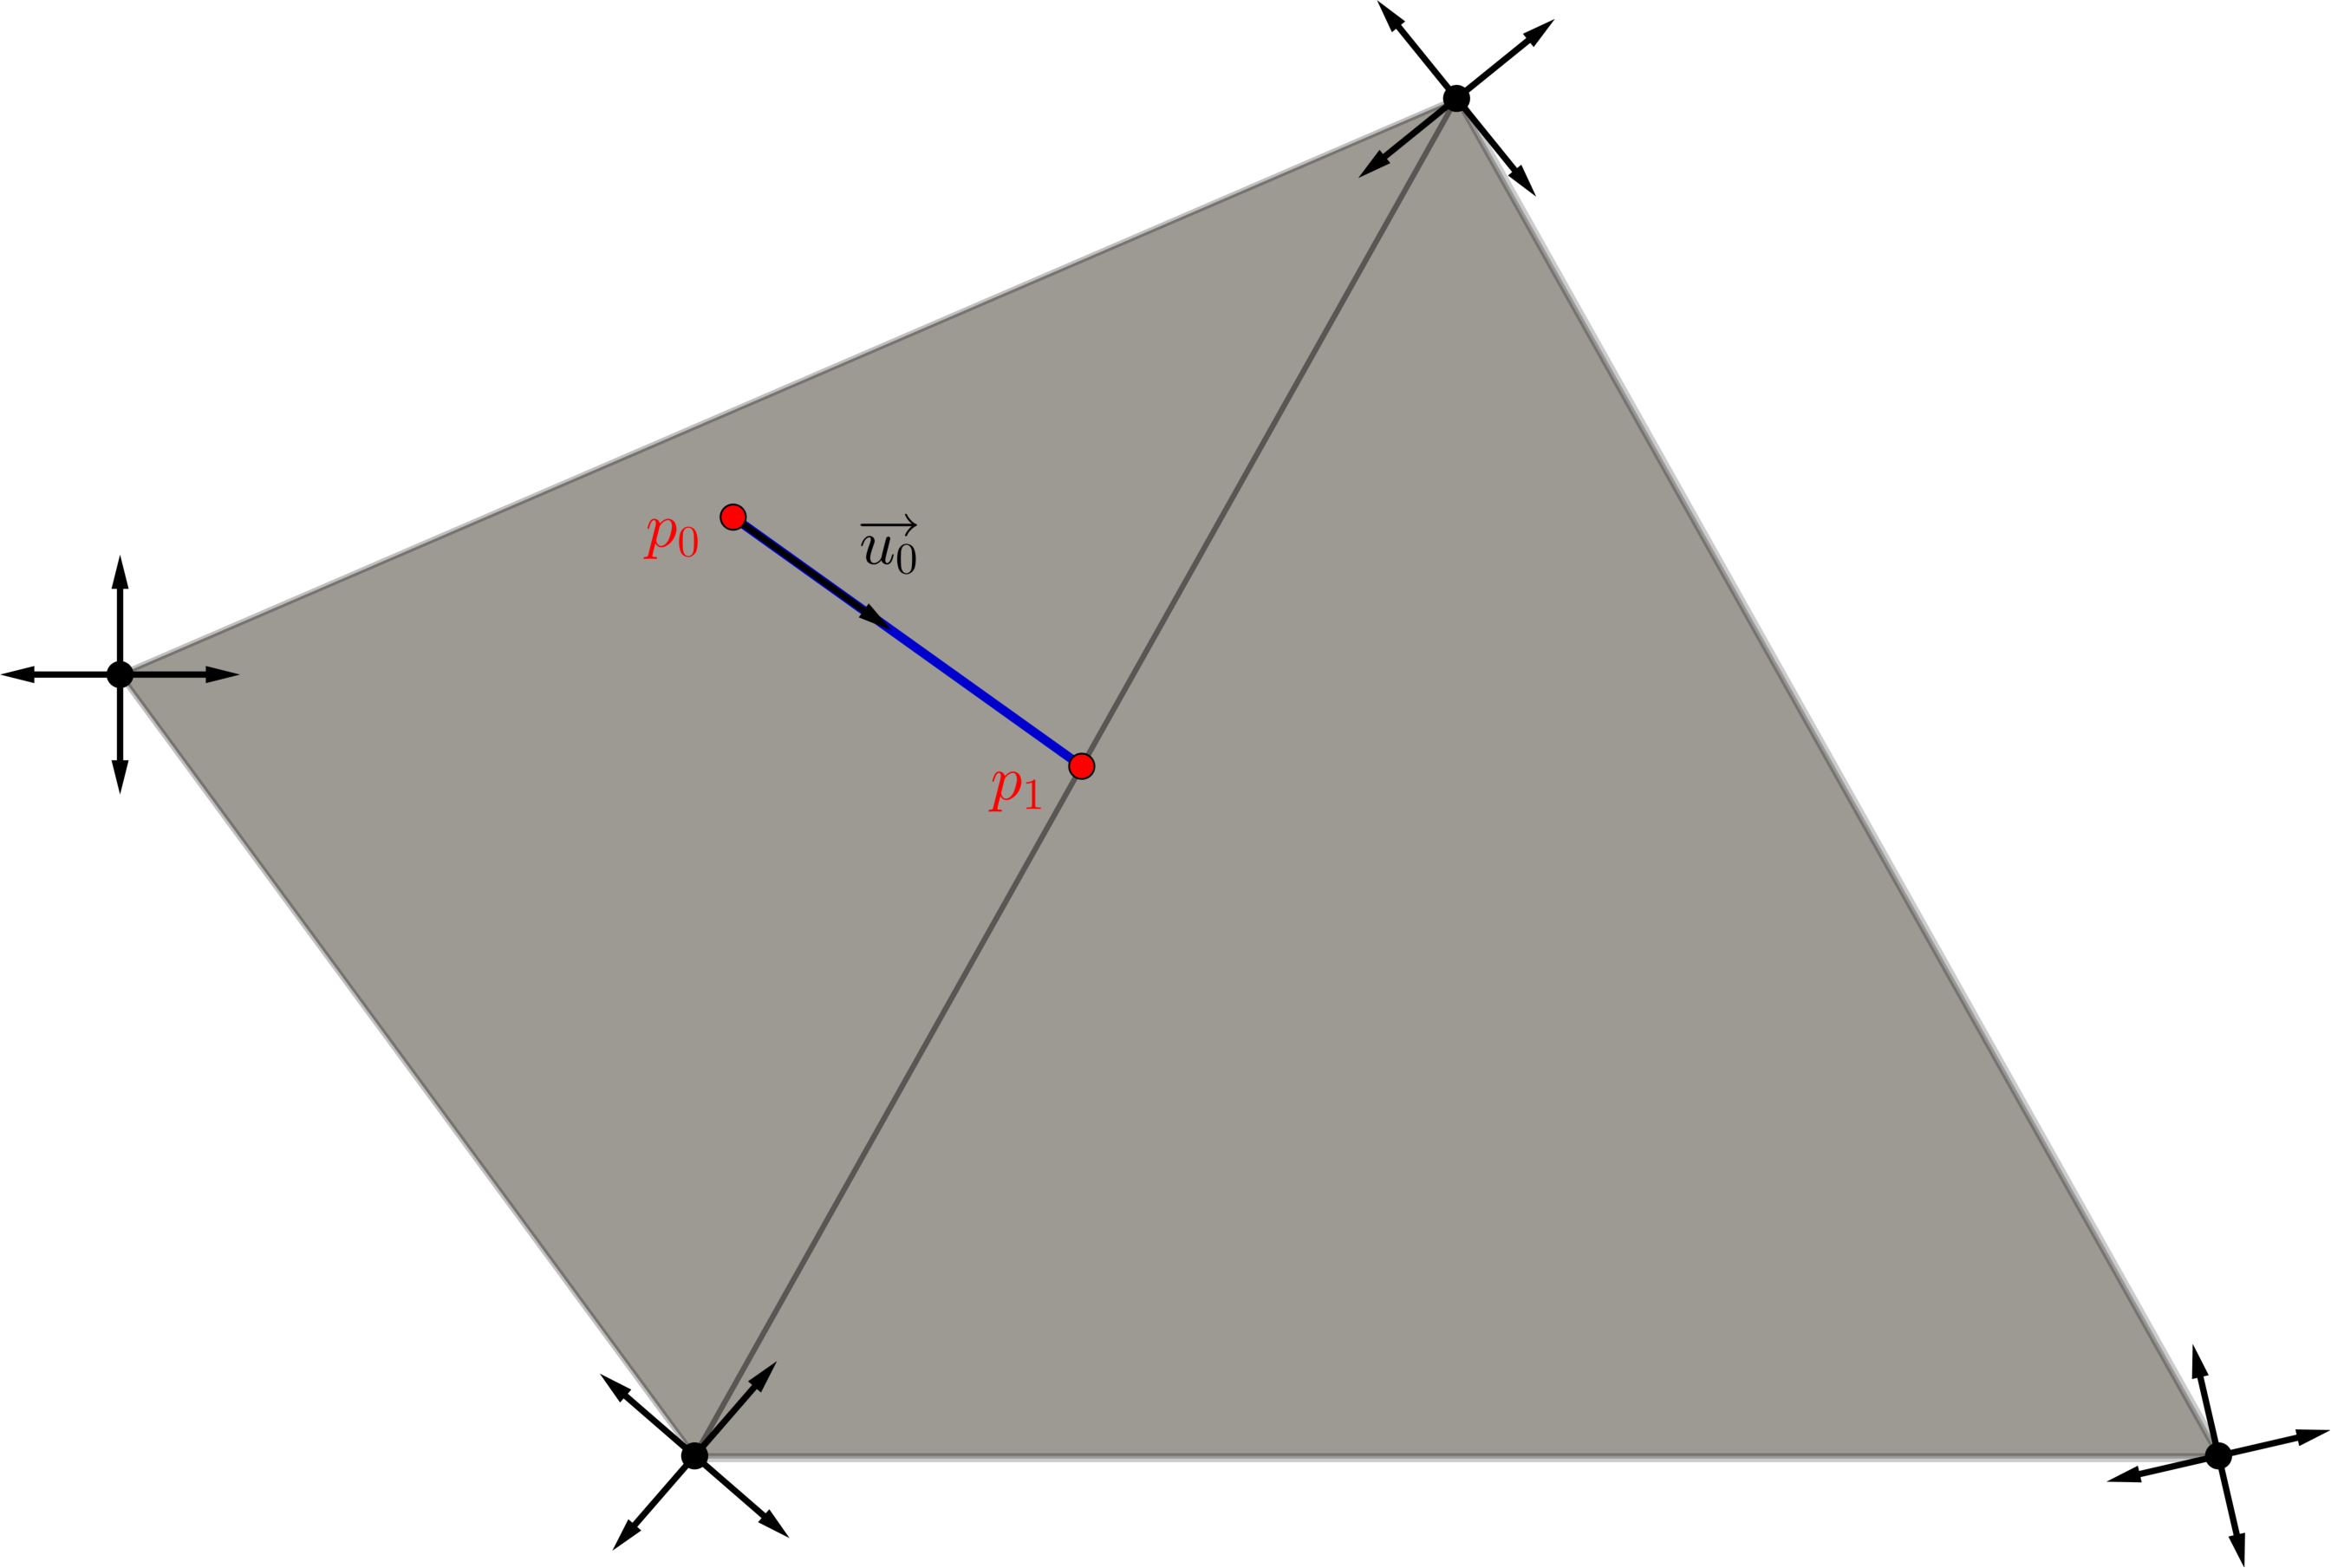
\includegraphics[width=\textwidth]{images/draw_streams_11.pdf}
         \caption{Construction du premier segment de la ligne de champ.}
     \end{subfigure}
     \begin{subfigure}[b]{0.7\textwidth}
         \centering
         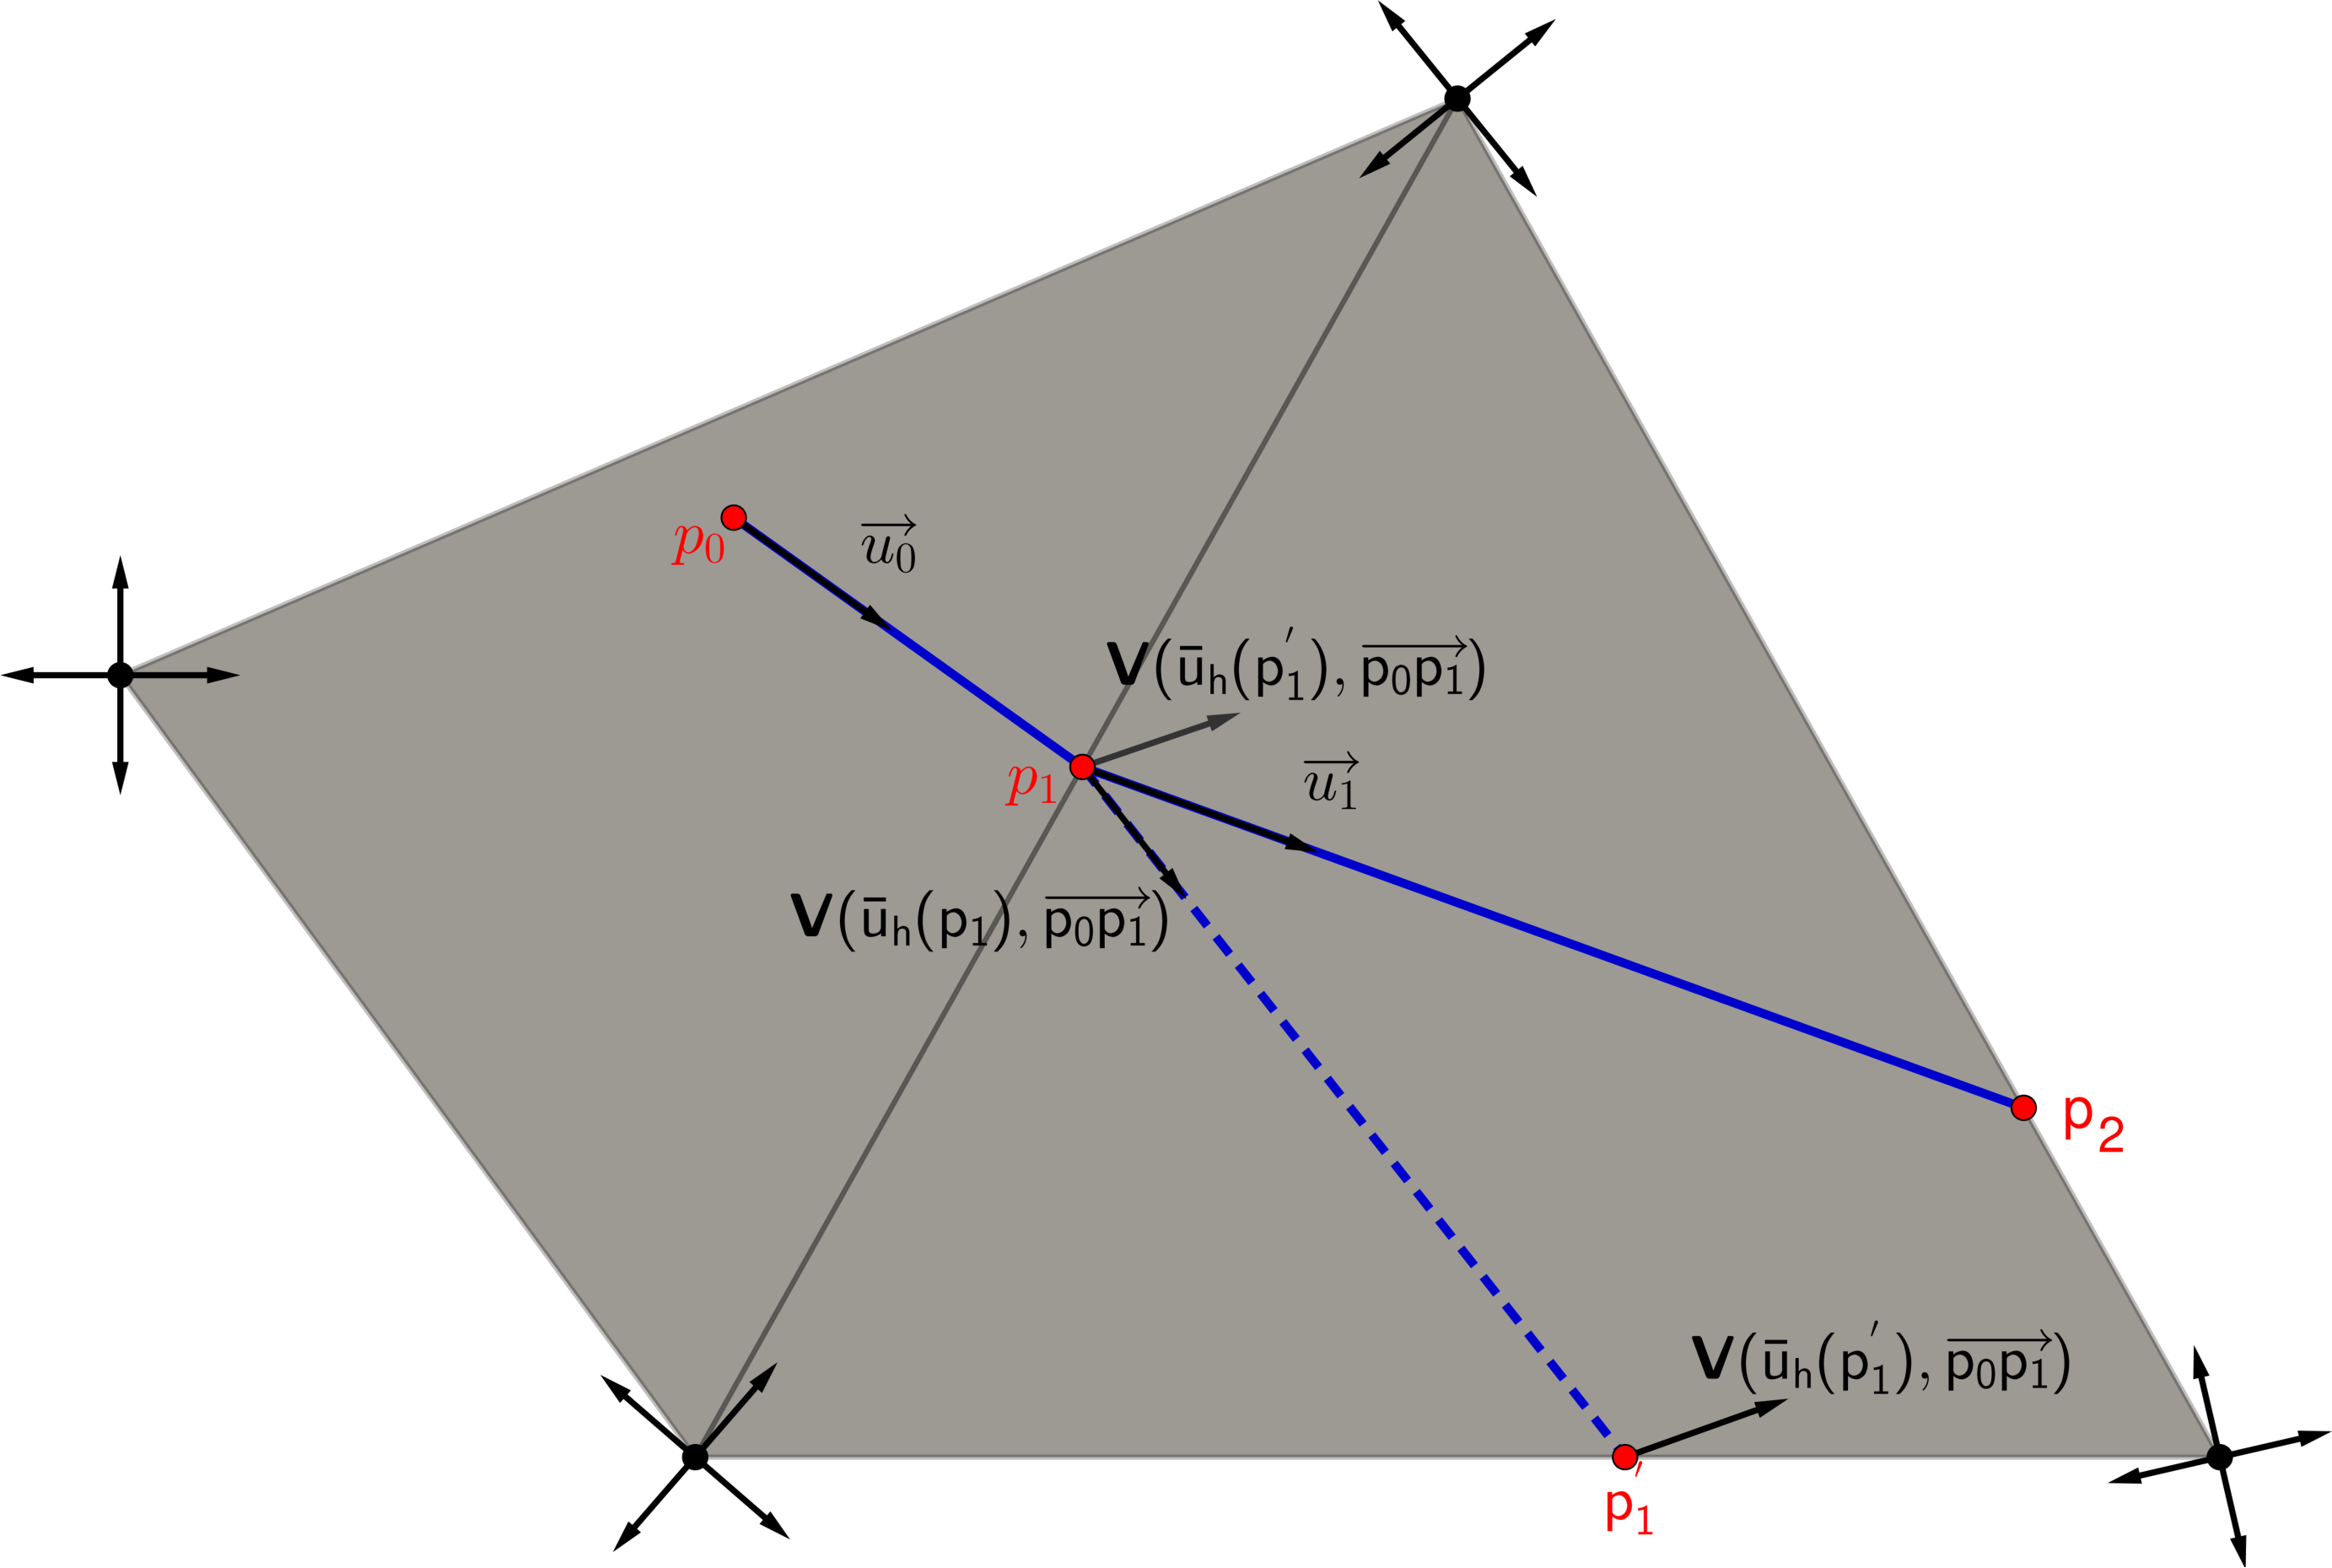
\includegraphics[width=\textwidth]{images/draw_streams_12.pdf}
         \caption{Intégration de la ligne de champ dans un triangle.}
     \end{subfigure}
        \caption{Approximation d'une ligne de champ par la méthode de Heun's.}
        \label{fig:draw_streams_1}
\end{figure}

Une approche alternative, plus efficace et rapide pour construire les segments $[p_ip_{i+1}]$ pour $i\geq 1$, consiste à exploiter la proposition \ref{prop:align_sepa_voisinnage}. Considérons $L_T=SL_{\bar{u}_h}\cap T$, la portion de la ligne de champ $SL_{\bar{u}_h}$ se trouvant dans un triangle $T$ et que l'on souhaite représenter par un segment $[p_ip_{i+1}]$. Ici, $p_i$ et $p_{i+1}$ représentent les points d'intersection entre $L$ et le bord de $T$ (c'est-à-dire, $\{p_i, p_{i+1}\}=L\cap\partial T$) et le but est de trouver le point $p_{i+1}$. Or d'après la proposition \ref{prop:align_sepa_voisinnage}, nous savons que pour tout $p\in L_T$ on a:
\begin{equation}
W^\gamma_{\bar{u}_h}(p_{i+1})-W^\gamma_{\bar{u}_h}(p_i)=-\pi,
\label{eqn:formule_W}
\end{equation}
où $\gamma$ est une paramétrisation sur $[0, 1]$ de $\partial T$ dans le sens positif et pour tout $t\in[0, 1]$ on a $W^\gamma_{\bar{u}_h}(t)=\theta_{\bar{u}_h}^\gamma(t)-\arg{\overrightarrow{p\gamma(t)}}$. Il suffit donc de trouver une approximation du point $p$ puis d'exploiter l'équation \ref{eqn:formule_W} pour trouver une approximation de $p_{i+1}$. Dans notre cas, nous choisissons comme approximation du point $p$, le point $p_i^{'}$ vérifiant:
$$
p_i^{'}\in T\mbox{ et }\overrightarrow{p_ip_i^{'}}=\epsilon\overrightarrow{p_{i-1}p_i}, \mbox{ avec }\epsilon\in]0, 1[.
$$
On trouve ensuite $p_{i+1}$ en utilisant l'équation \ref{eqn:formule_W} avec $W^\gamma_{\bar{u}_h}(t)=\theta_{\bar{u}_h}^\gamma(t)-\arg{\overrightarrow{p_i^{'}\gamma(t)}}$ (voir la figure \ref{fig:draw_streams_2}).

\begin{figure}[!h]
     \centering
     \begin{subfigure}[b]{0.7\textwidth}
         \centering
         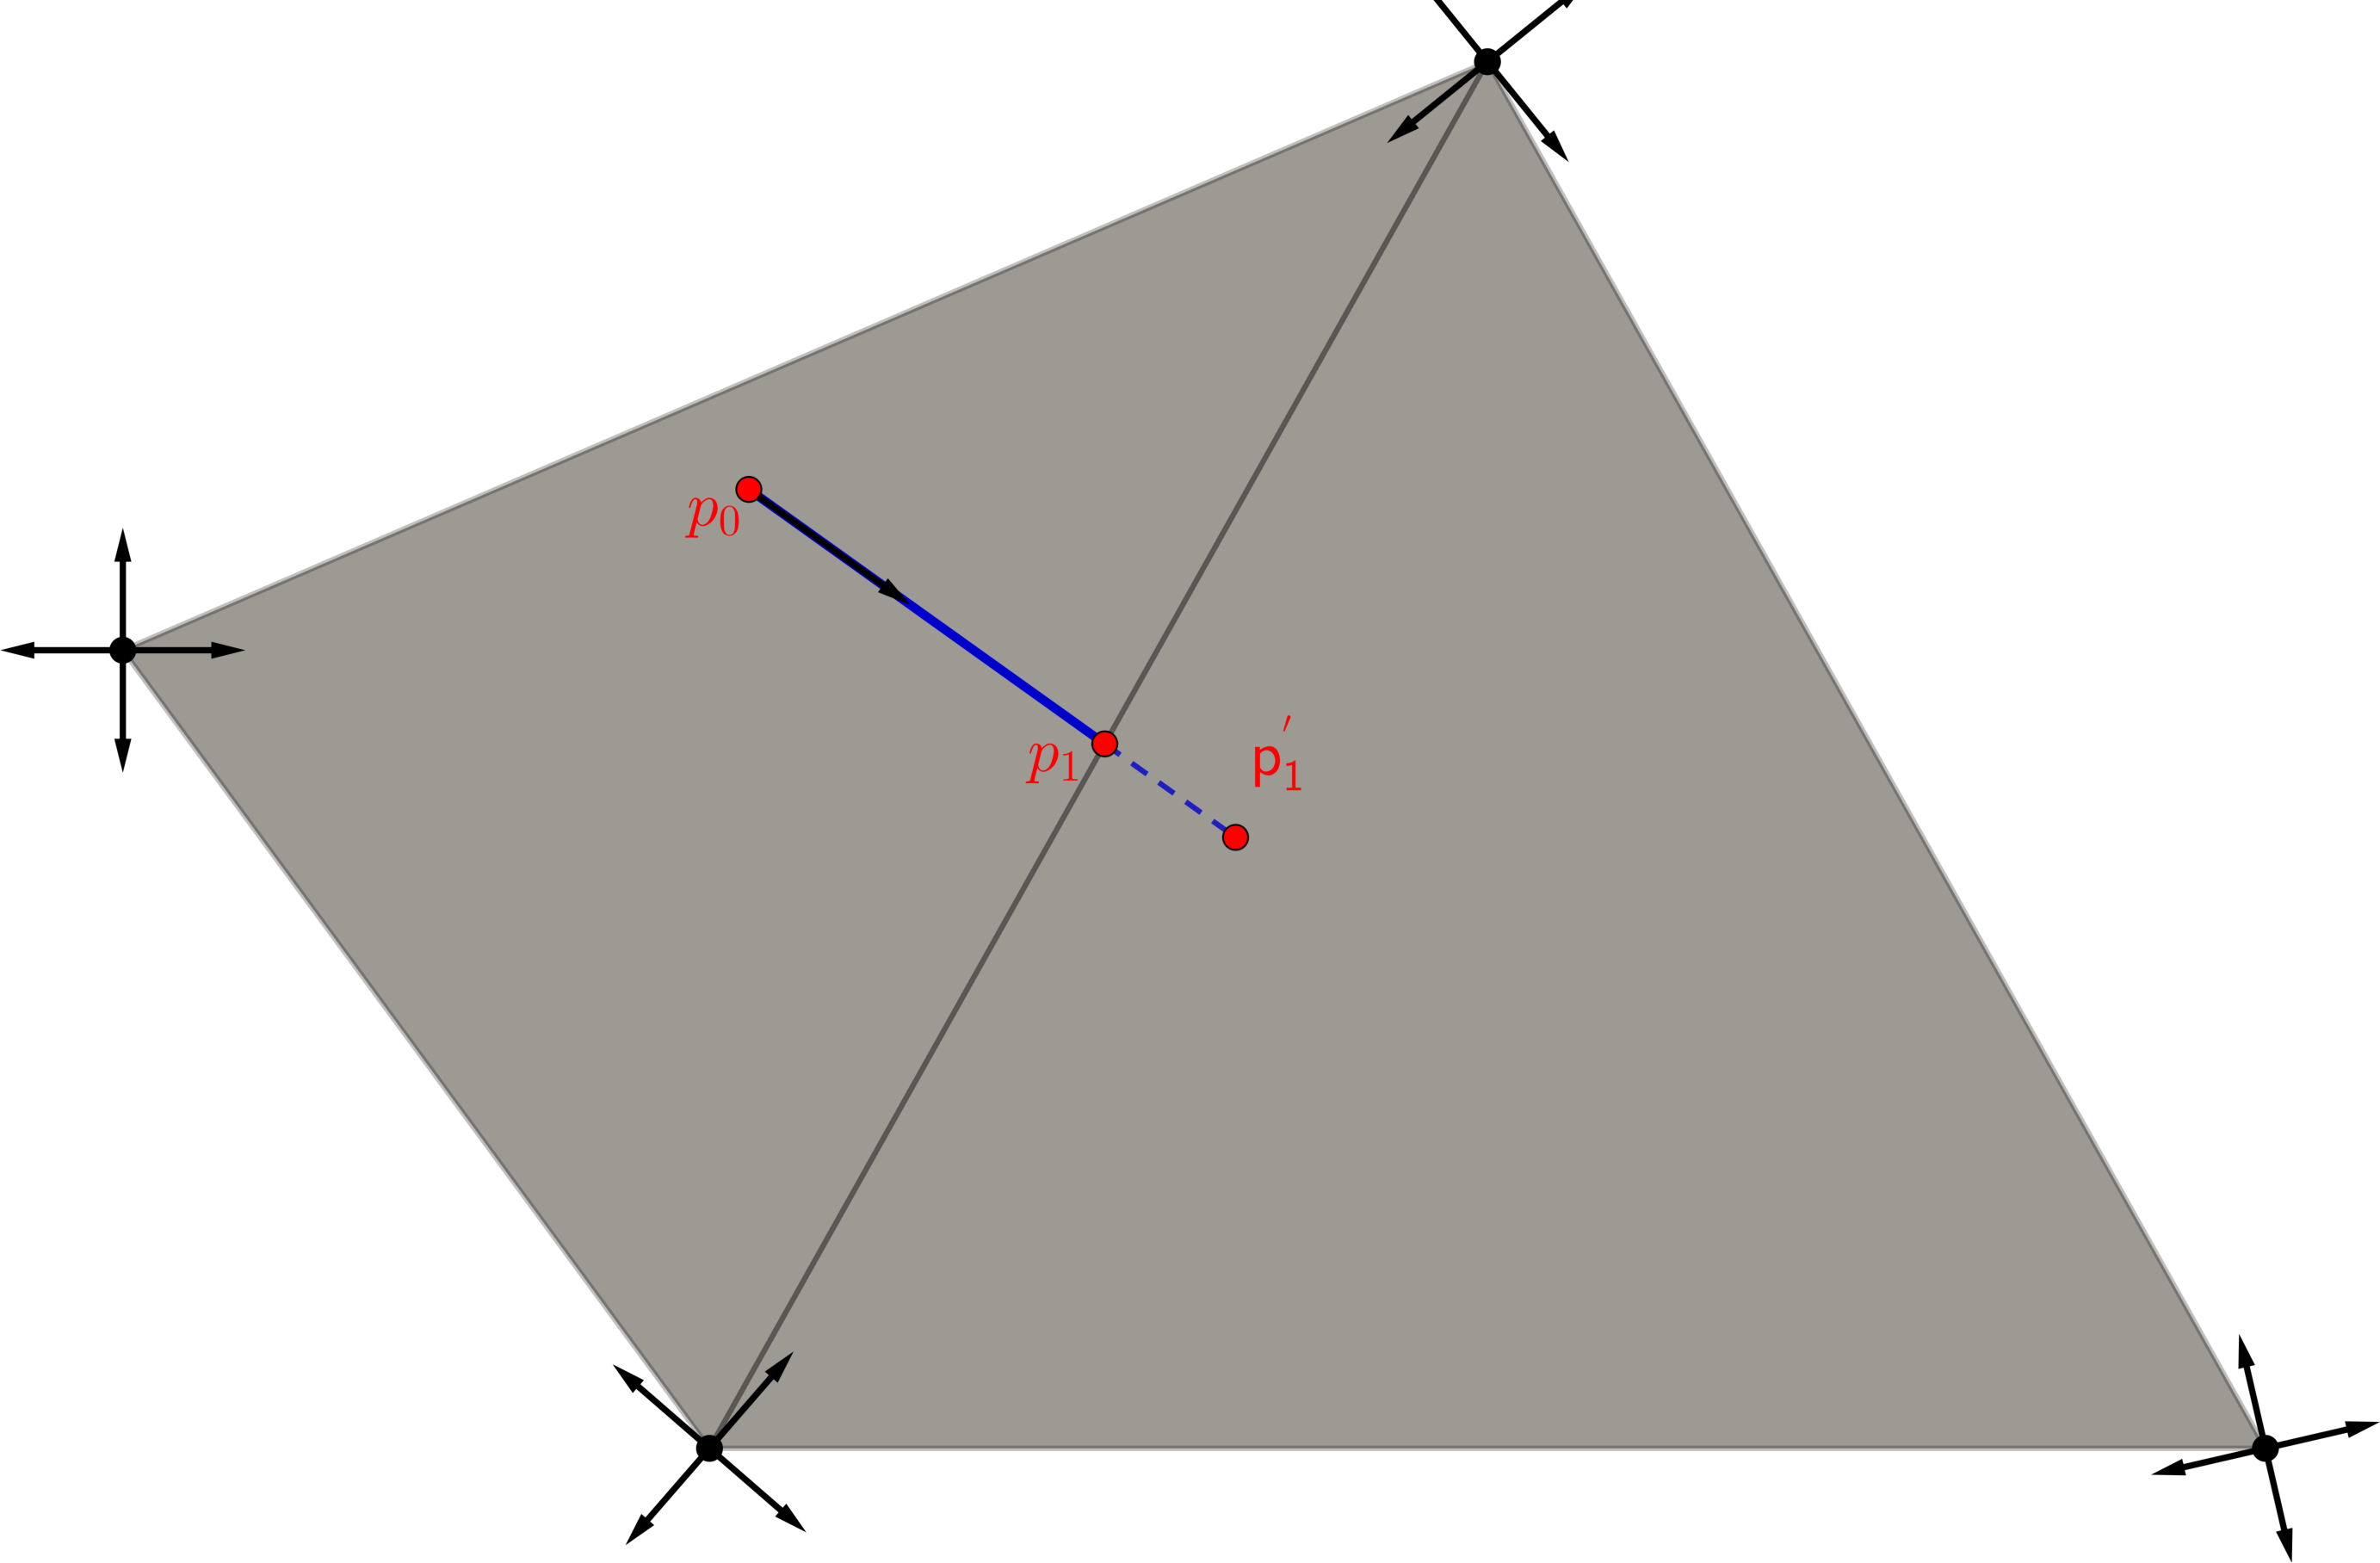
\includegraphics[width=\textwidth]{images/draw_streams_21.pdf}
         \caption{Construction du premier segment de la ligne de champ.}
     \end{subfigure}
     \begin{subfigure}[b]{0.7\textwidth}
         \centering
         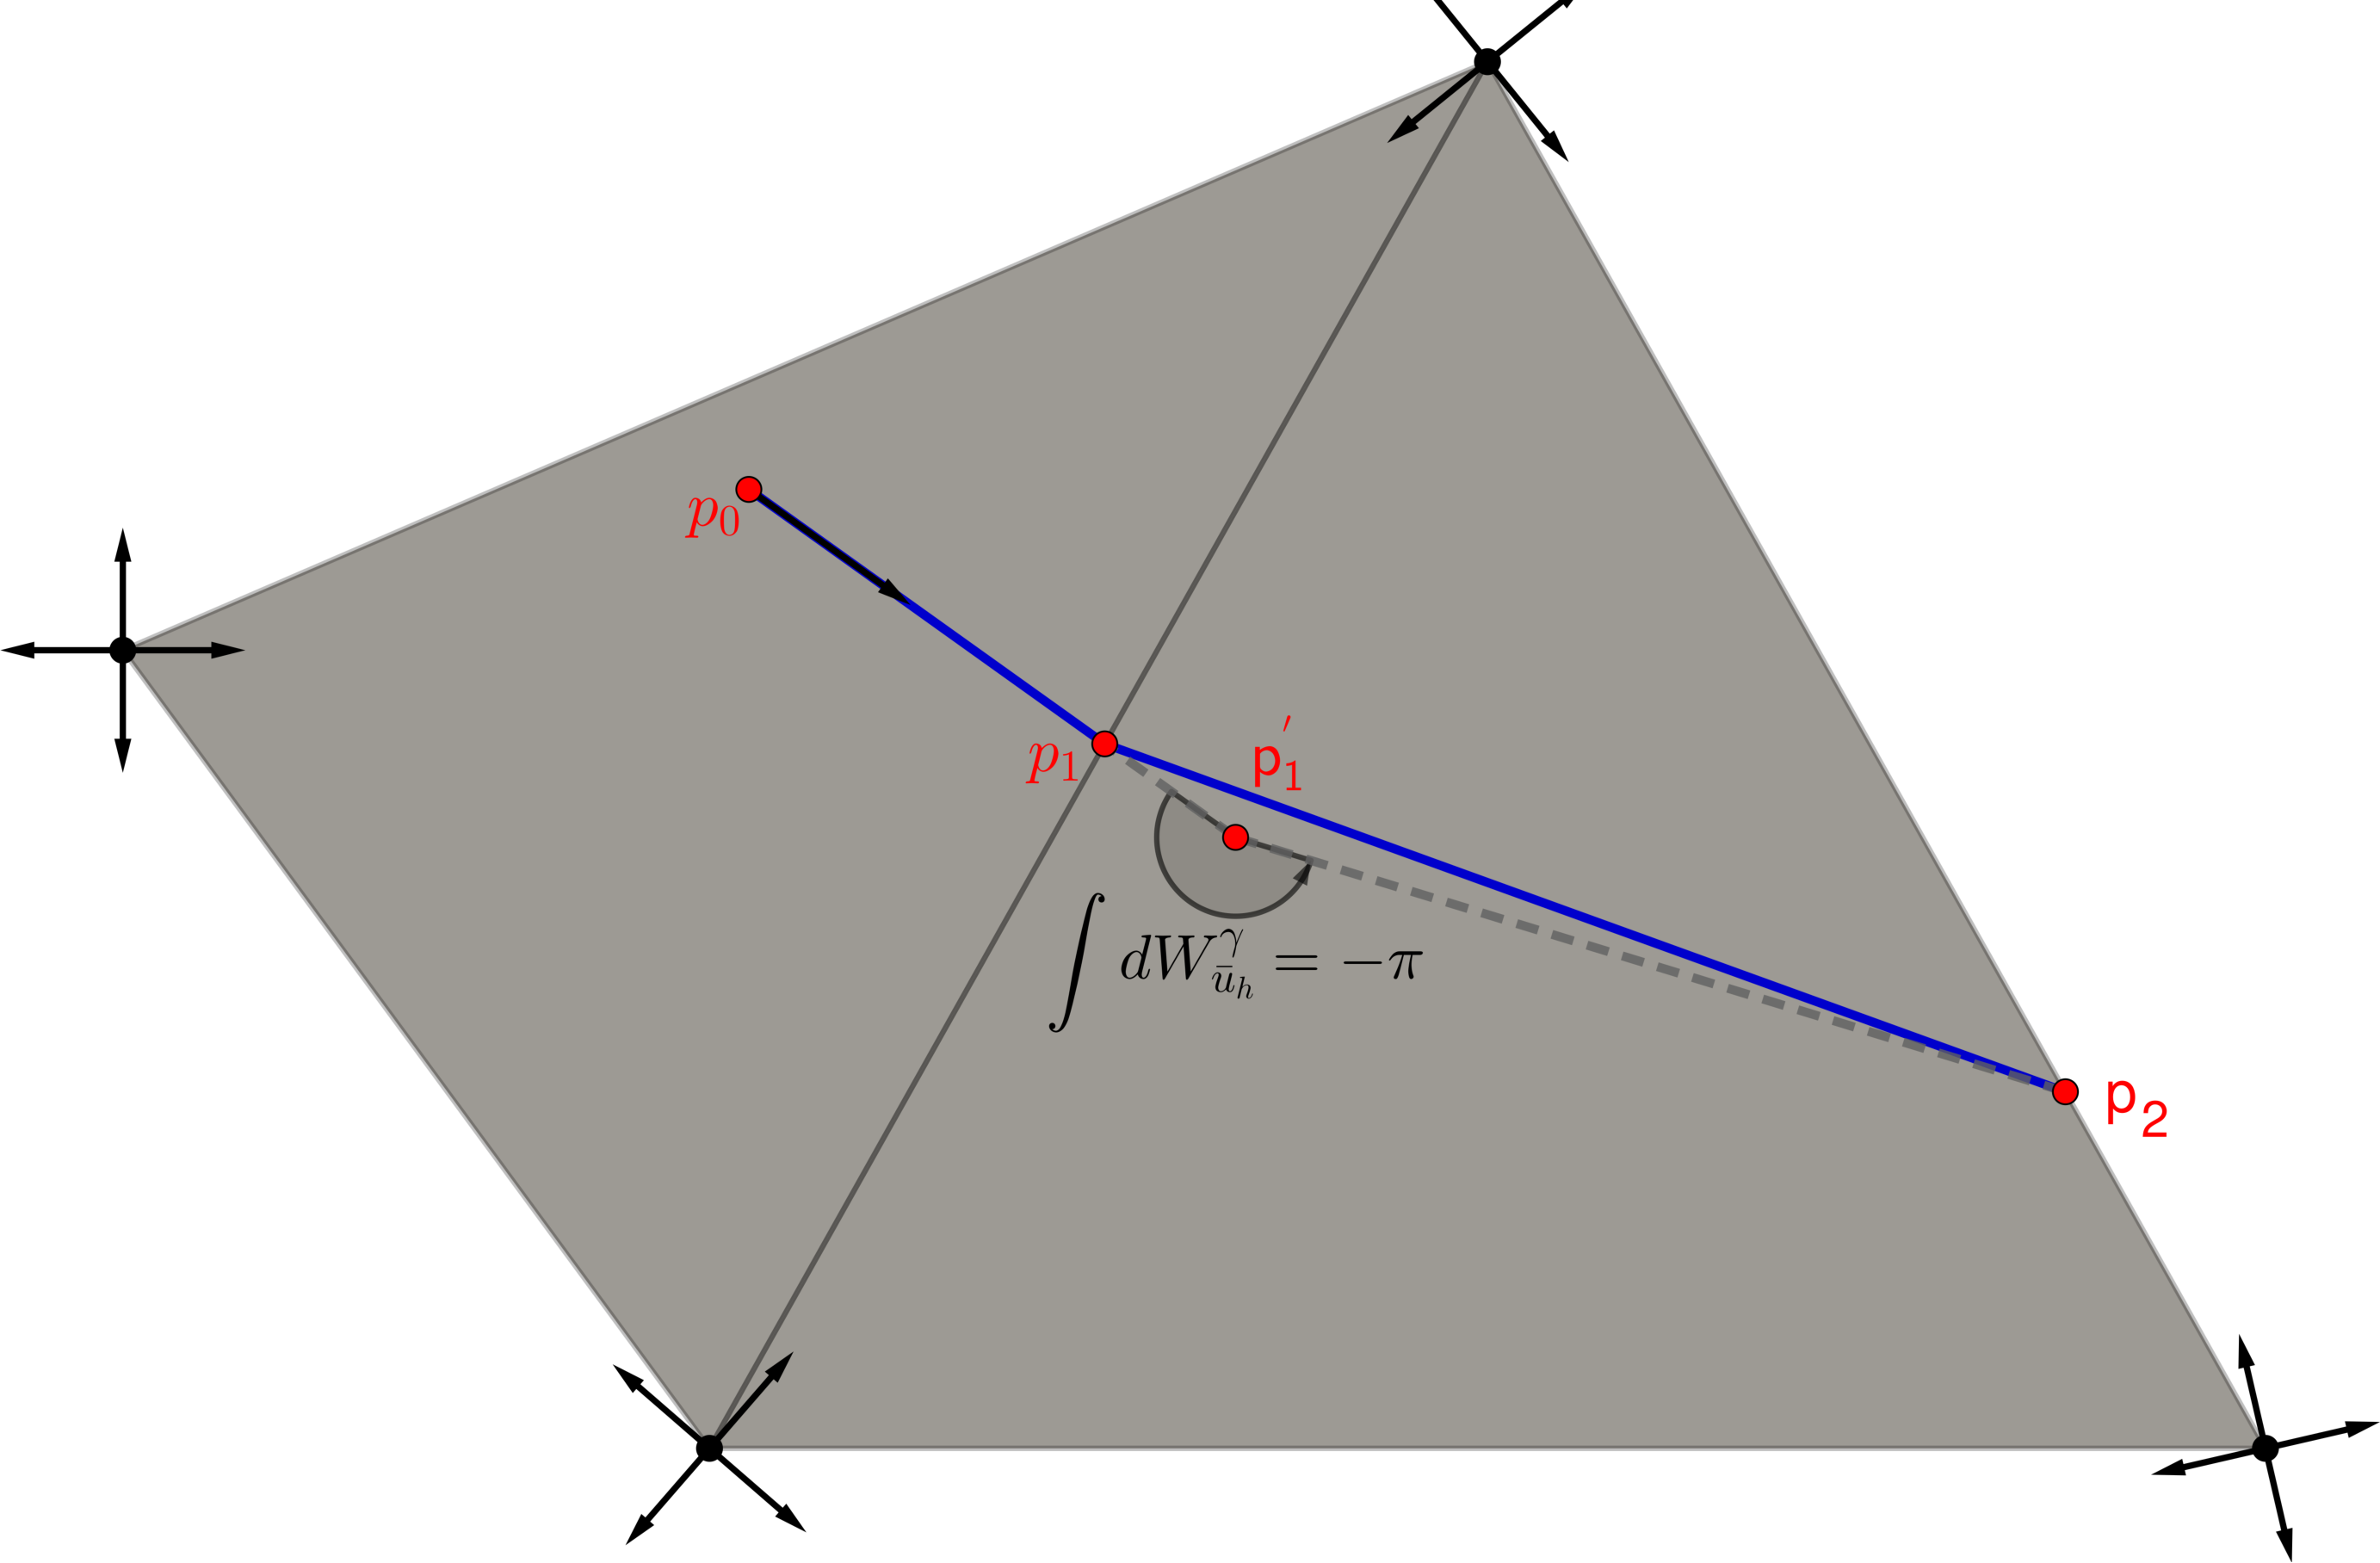
\includegraphics[width=\textwidth]{images/draw_streams_22.pdf}
         \caption{Intégration de la ligne de champ dans un triangle.}
     \end{subfigure}
        \caption{Approche alternative pour l'intéfration des lignes de champ dans un champ de croix.}
        \label{fig:draw_streams_2}
\end{figure}


\subsection{Lien entre $\bar{u}$ et $\bar{u}_h$}

À présent, nous nous posons la question de savoir quel lien on peut exhiber entre le champ de coix $\bar{u}$ et sa représentation $\bar{u}_h$ construite dans les parties précedentes.

Pour tout $T\in\mathcal{T}_h$ avec $T$ non-singulier, on sait que $\theta_{\bar{u}_h}$ est linéaire par construction dans $T$. Il vient alors que $\theta_{\bar{u}_h}$ tend vers $\theta_{\bar{u}}$ sur $\Omega_h\backslash\cup_{p\in\mathcal{S}_{\bar{u}_h}}T_p$ lorsque $h$ tend vers $0$. Autrement dit, $\bar{u}_h$ tend vers $\bar{u}$ sur $\Omega_h\backslash\cup_{p\in\mathcal{S}_{\bar{u}_h}}T_p$ lorsque $h$ tend vers $0$. \color{red} Cependant la somme des indices des points singuliers de $u$ est équivalent à la somme des indices des points singuliers de $\bar{u}_h$.\color{black}.
\[\]
Une conséquence de la représentation du champ de croix que nous avons présentée est que les points singuliers de $\bar{u}$ ne correspondent pas aux points singuliers de $\bar{u}_h$ ($\mathcal{S}_{\bar{u}}=\mathcal{S}_{\bar{u}_h}$). Par exemple, sur la figure \ref{fig:eclatement_point_sing}, nous avons un champ de croix contenant un point singulier d'indice $1$ que nous représentons sur un maillage triangulaire. On observe alors la présence d'une multitude de points singuliers d'indice $1/4$ et d'indices $-1/4$, localisés dans divers triangles. Il est à noter cependant que la somme des indices de ces points singuliers correspond bien à l'indice du point singulier initial. D'où le lemme suivant:

\begin{lemma}
 Soit $\bar{u}_h$ une représentation de $\bar{u}$ sur $\Omega_h$. Alors on a:
 $$
 \sum_{p\in\mathcal{S}_{\bar{u}}\backslash\partial\Omega}id_{\bar{u}}(p)=\sum_{p\in\mathcal{S}_{\bar{u}_h}\backslash\partial\Omega_h}id_{\bar{u}_h}(p).
 $$
\end{lemma}

\begin{proof}

\end{proof}


\begin{figure}[!h]
  \centering
  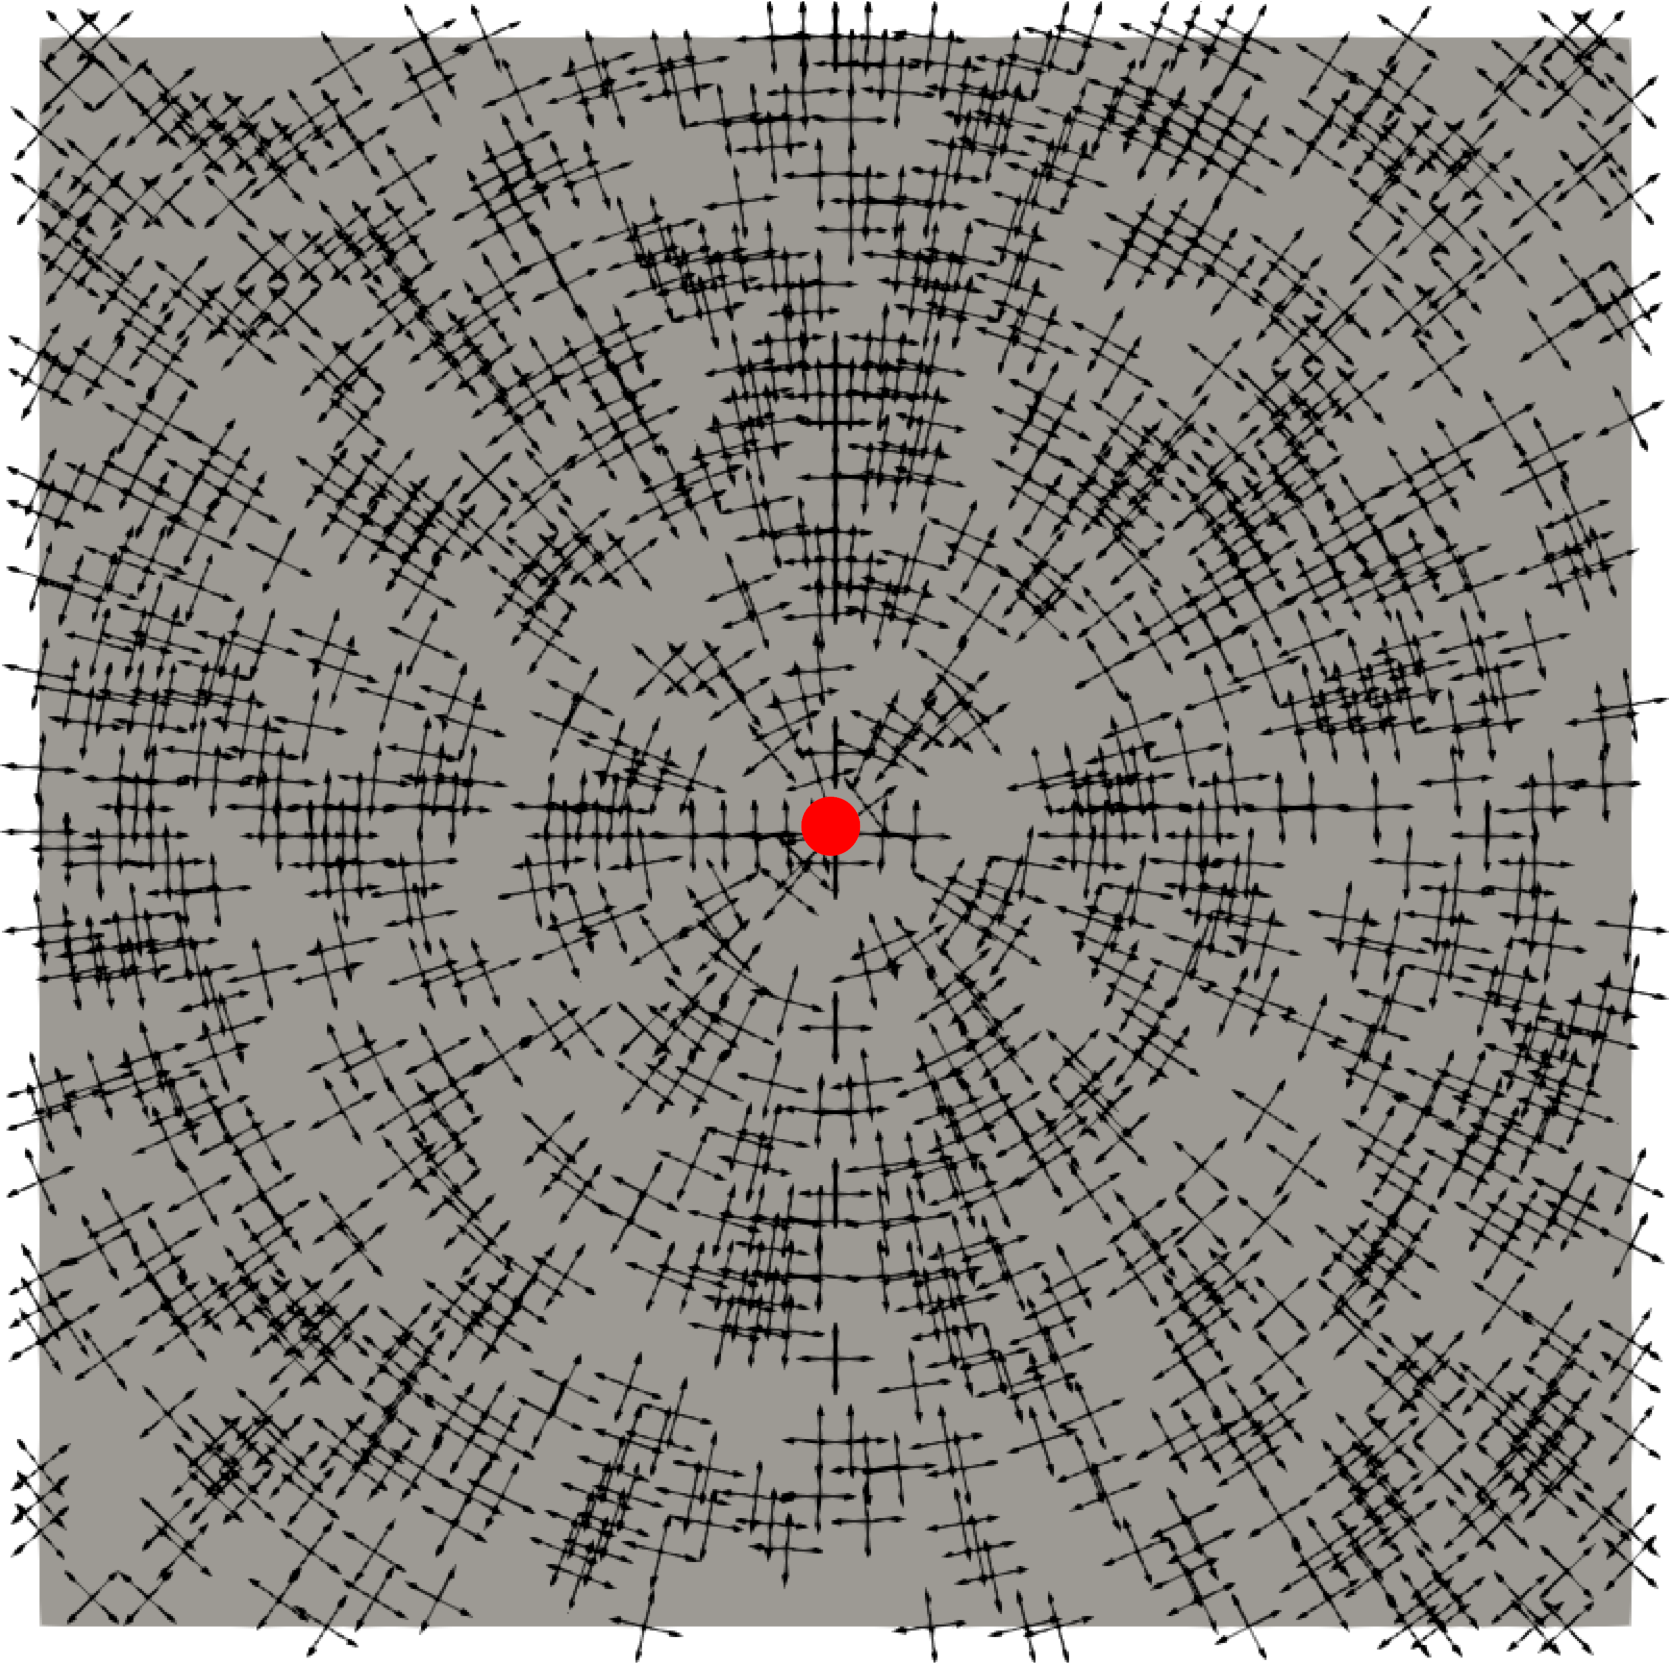
\includegraphics[scale=0.27]{images/u_sing.pdf}\hspace{0.2cm}
  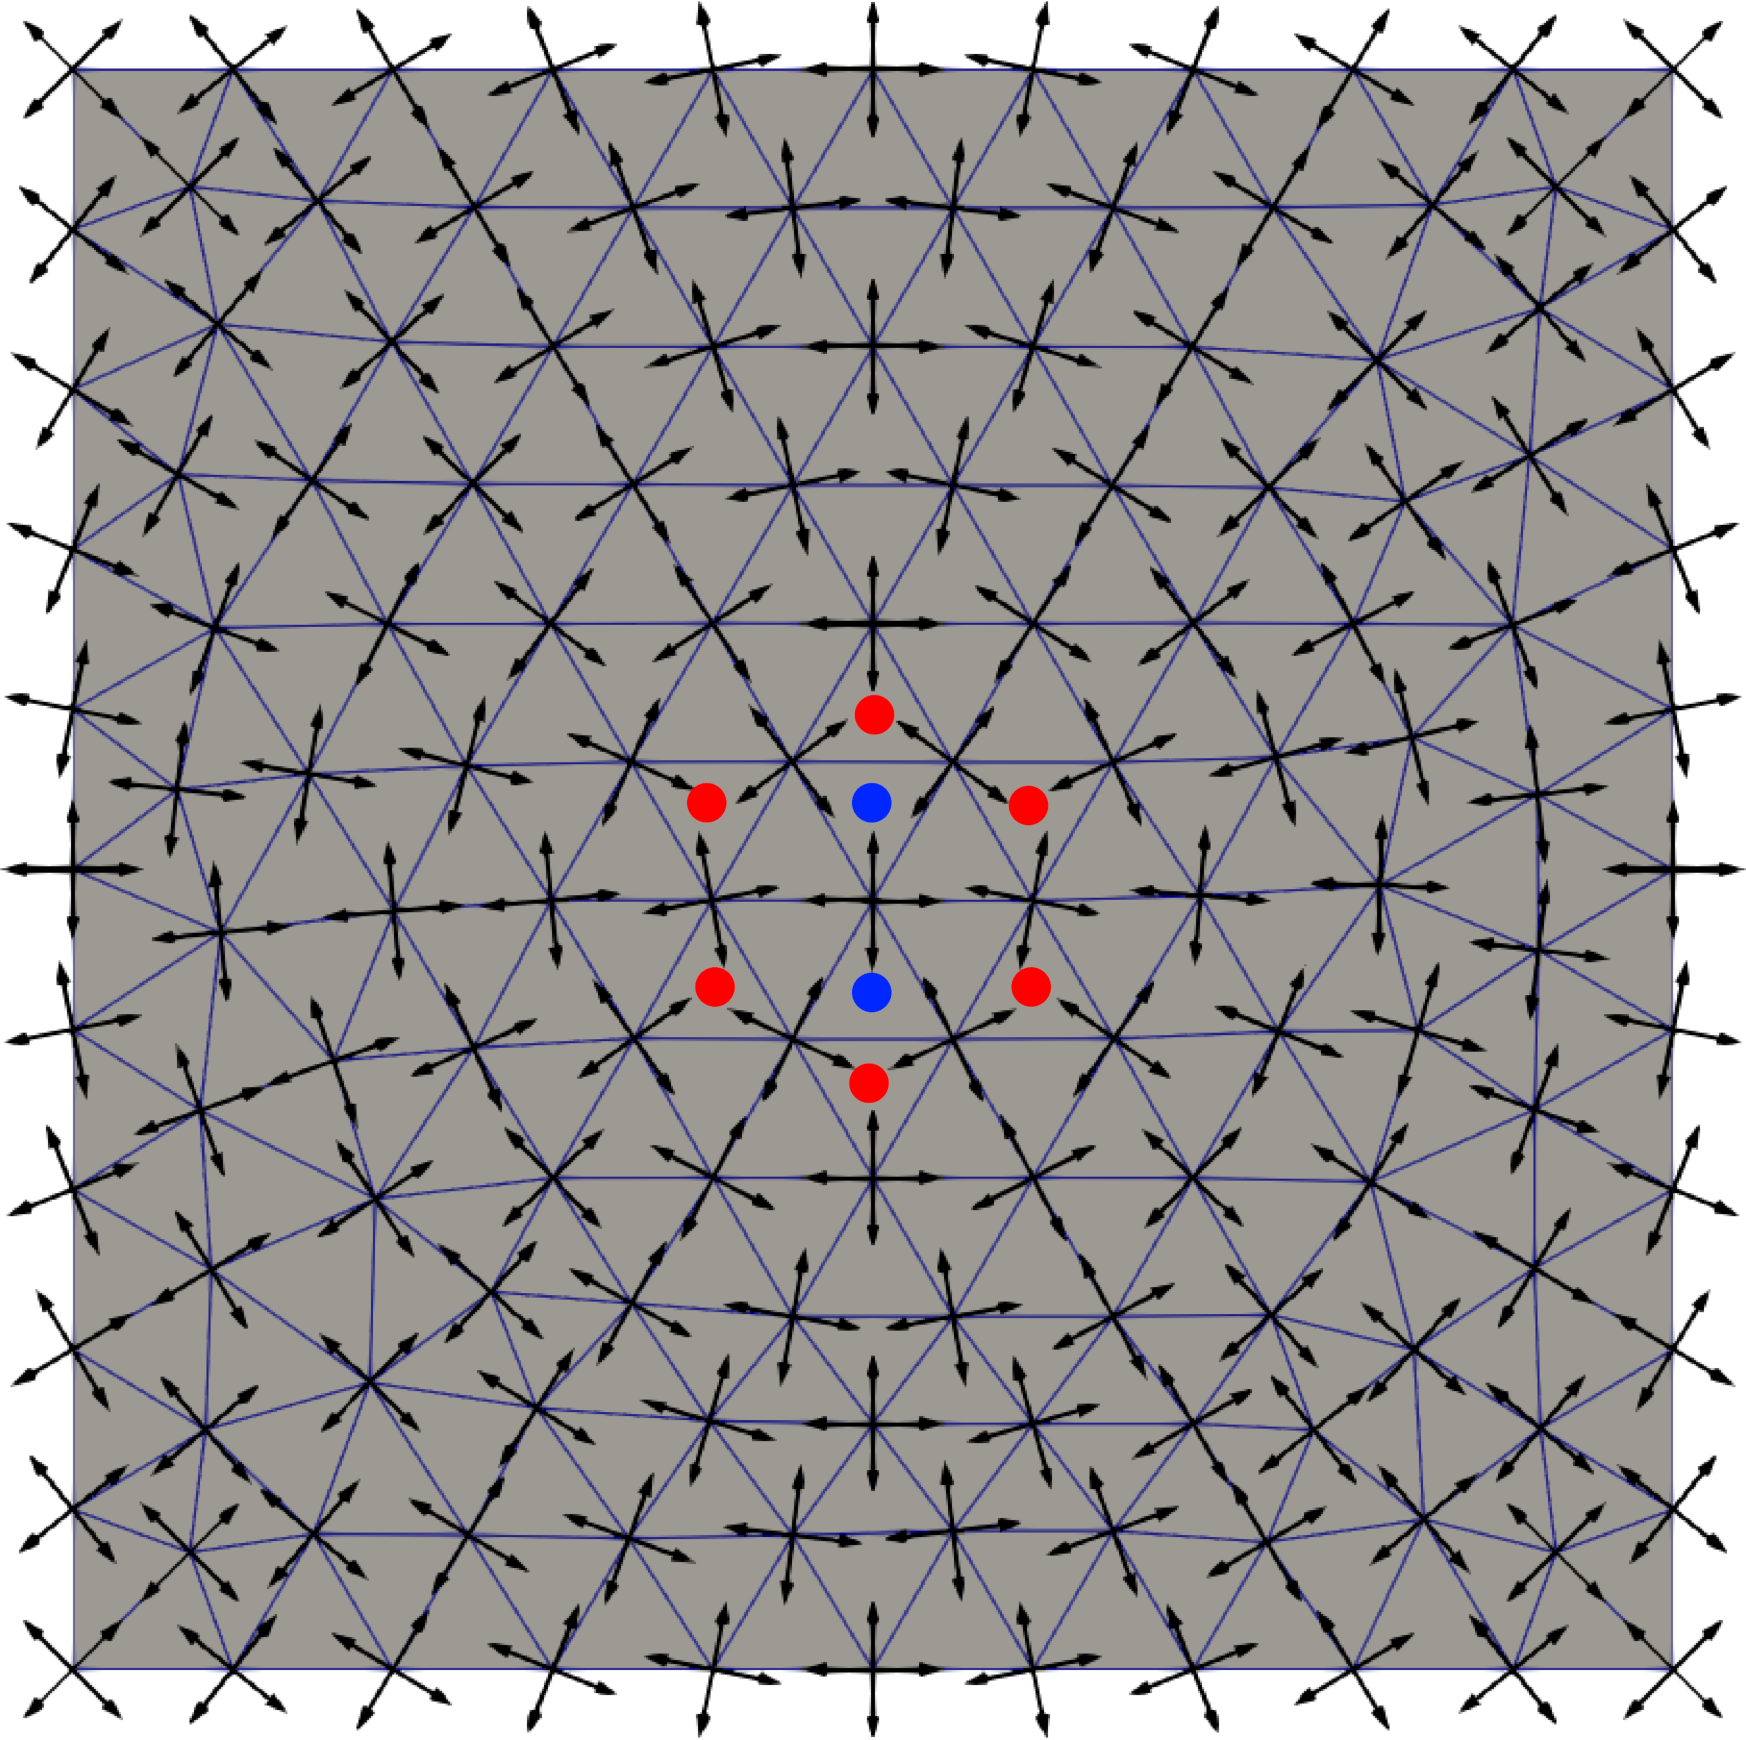
\includegraphics[scale=0.26]{images/u_h_sing.pdf}
  \caption{.}
  \label{fig:eclatement_point_sing}
\end{figure}

\section{Partitionnement de $\partial\Omega_h$}

L'adaptation de l'algorithme de partitionnement \ref{alg:algo_main} au maillage $\Omega_h$ est donné par:\\

\begin{algorithm}[H]
\label{alg:discr_algo_main}
\SetKwInOut{Input}{Entrée}
\SetKwInOut{Output}{Sortie}
\Input{$\Omega_h$ un maillage triangulaire, champ de croix $\bar{u}_h$ linéaire par morceau sur chaque triangle de $\Omega_h$.}
\Output{Partition de $\Omega_h$ en ensembles de régions.}
\vspace{0.2cm}
1.) Identification des points singuliers du champ de croix,\\\vspace{0.2cm}
2.) Détermination du nombre de séparatrices pour chaque point singulier,\\\vspace{0.2cm}
3.) Intégration des séparatrices,\\\vspace{0.2cm}
4.) Identification des régions.\\\vspace{0.2cm}
\caption{Algorithme de partitionnement $\Omega_h$}
\end{algorithm}
\vspace{0.5cm}
On considère que l'algorithme a convergé si les séparatrices ne convergent pas vers un cycle limite. Examinons maintenant en détail certaines étapes de cet algorithme:

\subsection{Recherche de points singuliers}

Par construction, les points singuliers du champ de croix $\bar{u}_h$ se situent soit aux sommets du maillage $\Omega_h$, soit à l'intérieur des triangles qui le constituent.En pratique, la recherche de ces points peut être effectuée localement sur chaque triangle. Cela implique de tester le caractère singulier ou non de chaque triangle (voir la définition \ref{def:triangle_singulier}). Considérons $T\in\mathcal{T}_h$ comme un triangle singulier de $\Omega_h$. Par conception, il contient nécessairement un point singulier. Nous distinguons alors deux cas :\\
\begin{itemize}
 \item le point singulier correspond à l'un des sommets du triangle $T$.\\
 \item sinon, le point singulier se trouve à l'intérieur du triangle. Conformément à notre représentation de $\bar{u}_h$, dans ce cas précis, il s'agit du barycentre du triangle. Cependant rien empêche de choisir un autre point à l'intérieur du triangle tout en modifiant le calcul des valeurs du champ dans le triangle. Remarquons que tous les points singuliers de bord sont sur des sommets.\\
\end{itemize}

Une fois la localisation des points singulier identifié, on peut facilement calculé leur index grâce aux formules \ref{eqn:ind_int} ou \ref{eqn:ind_bord} en fonction de leur localisation.

\begin{remark}
L'emplacement d'un point singulier $p$ dans $T_p$ n'est pas fixé de manière absolue. La proposition \ref{prop:stream_from_interior_sing} indique qu'il est possible de faire correspondre ce point singulier à tout point à l'intérieur de $T_p$, moyennant une modification du champ dans $T_p$ comme spécifié dans ladite proposition. Dans notre représentation des champs de croix précédemment exposée, nous avons opté pour le barycentre des triangles lorsque $T_p$ correspond à un triangle.

En poursuivant cette logique, il est envisageable de substituer un groupe de singularités par un unique point singulier. Pour cela, il suffit de définir l'ensemble $T_p$ de manière à ce qu'il englobe tous les points singuliers que l'on souhaite regrouper avec $p$, le nouveau point singulier. Cette approche est bénéfique car elle permet de traiter les points singuliers situés trop près les uns des autres, par exemple, ceux présents dans deux triangles voisins.
\end{remark}

\subsection{Construction des séparatrices}

Une fois les points singuliers de $\bar{u}_h$ identifiés, nous procédons à la création des séparatrices sur $\Omega_h$. Cette étape comprend le calcul du nombre de séparatrices à assigner à chaque point singulier, la détermination des directions initiales pour chaque séparatrice, ainsi que l'intégration de ces séparatrices.

\paragraph{Nombre de séparatrices:} Si $p$ est un point singulier de $\bar{u}_h$, alors le nombre de séparatrices $N_s(p)$ associées à $p$ est donné par:
\begin{equation}
    N_s(p) = 
    \left\{
    \begin{array}{ll}
    4-4id_{\bar{u}_h}(p) & \mbox{ si } p\in\Omega_h\backslash\partial\Omega_h\\[0.3cm]
    2-4id_{\bar{u}_h}(p) & \mbox{ si } p\in\partial\Omega_h
    \end{array}
    \right.
\end{equation}

\begin{figure}[!h]
\centering
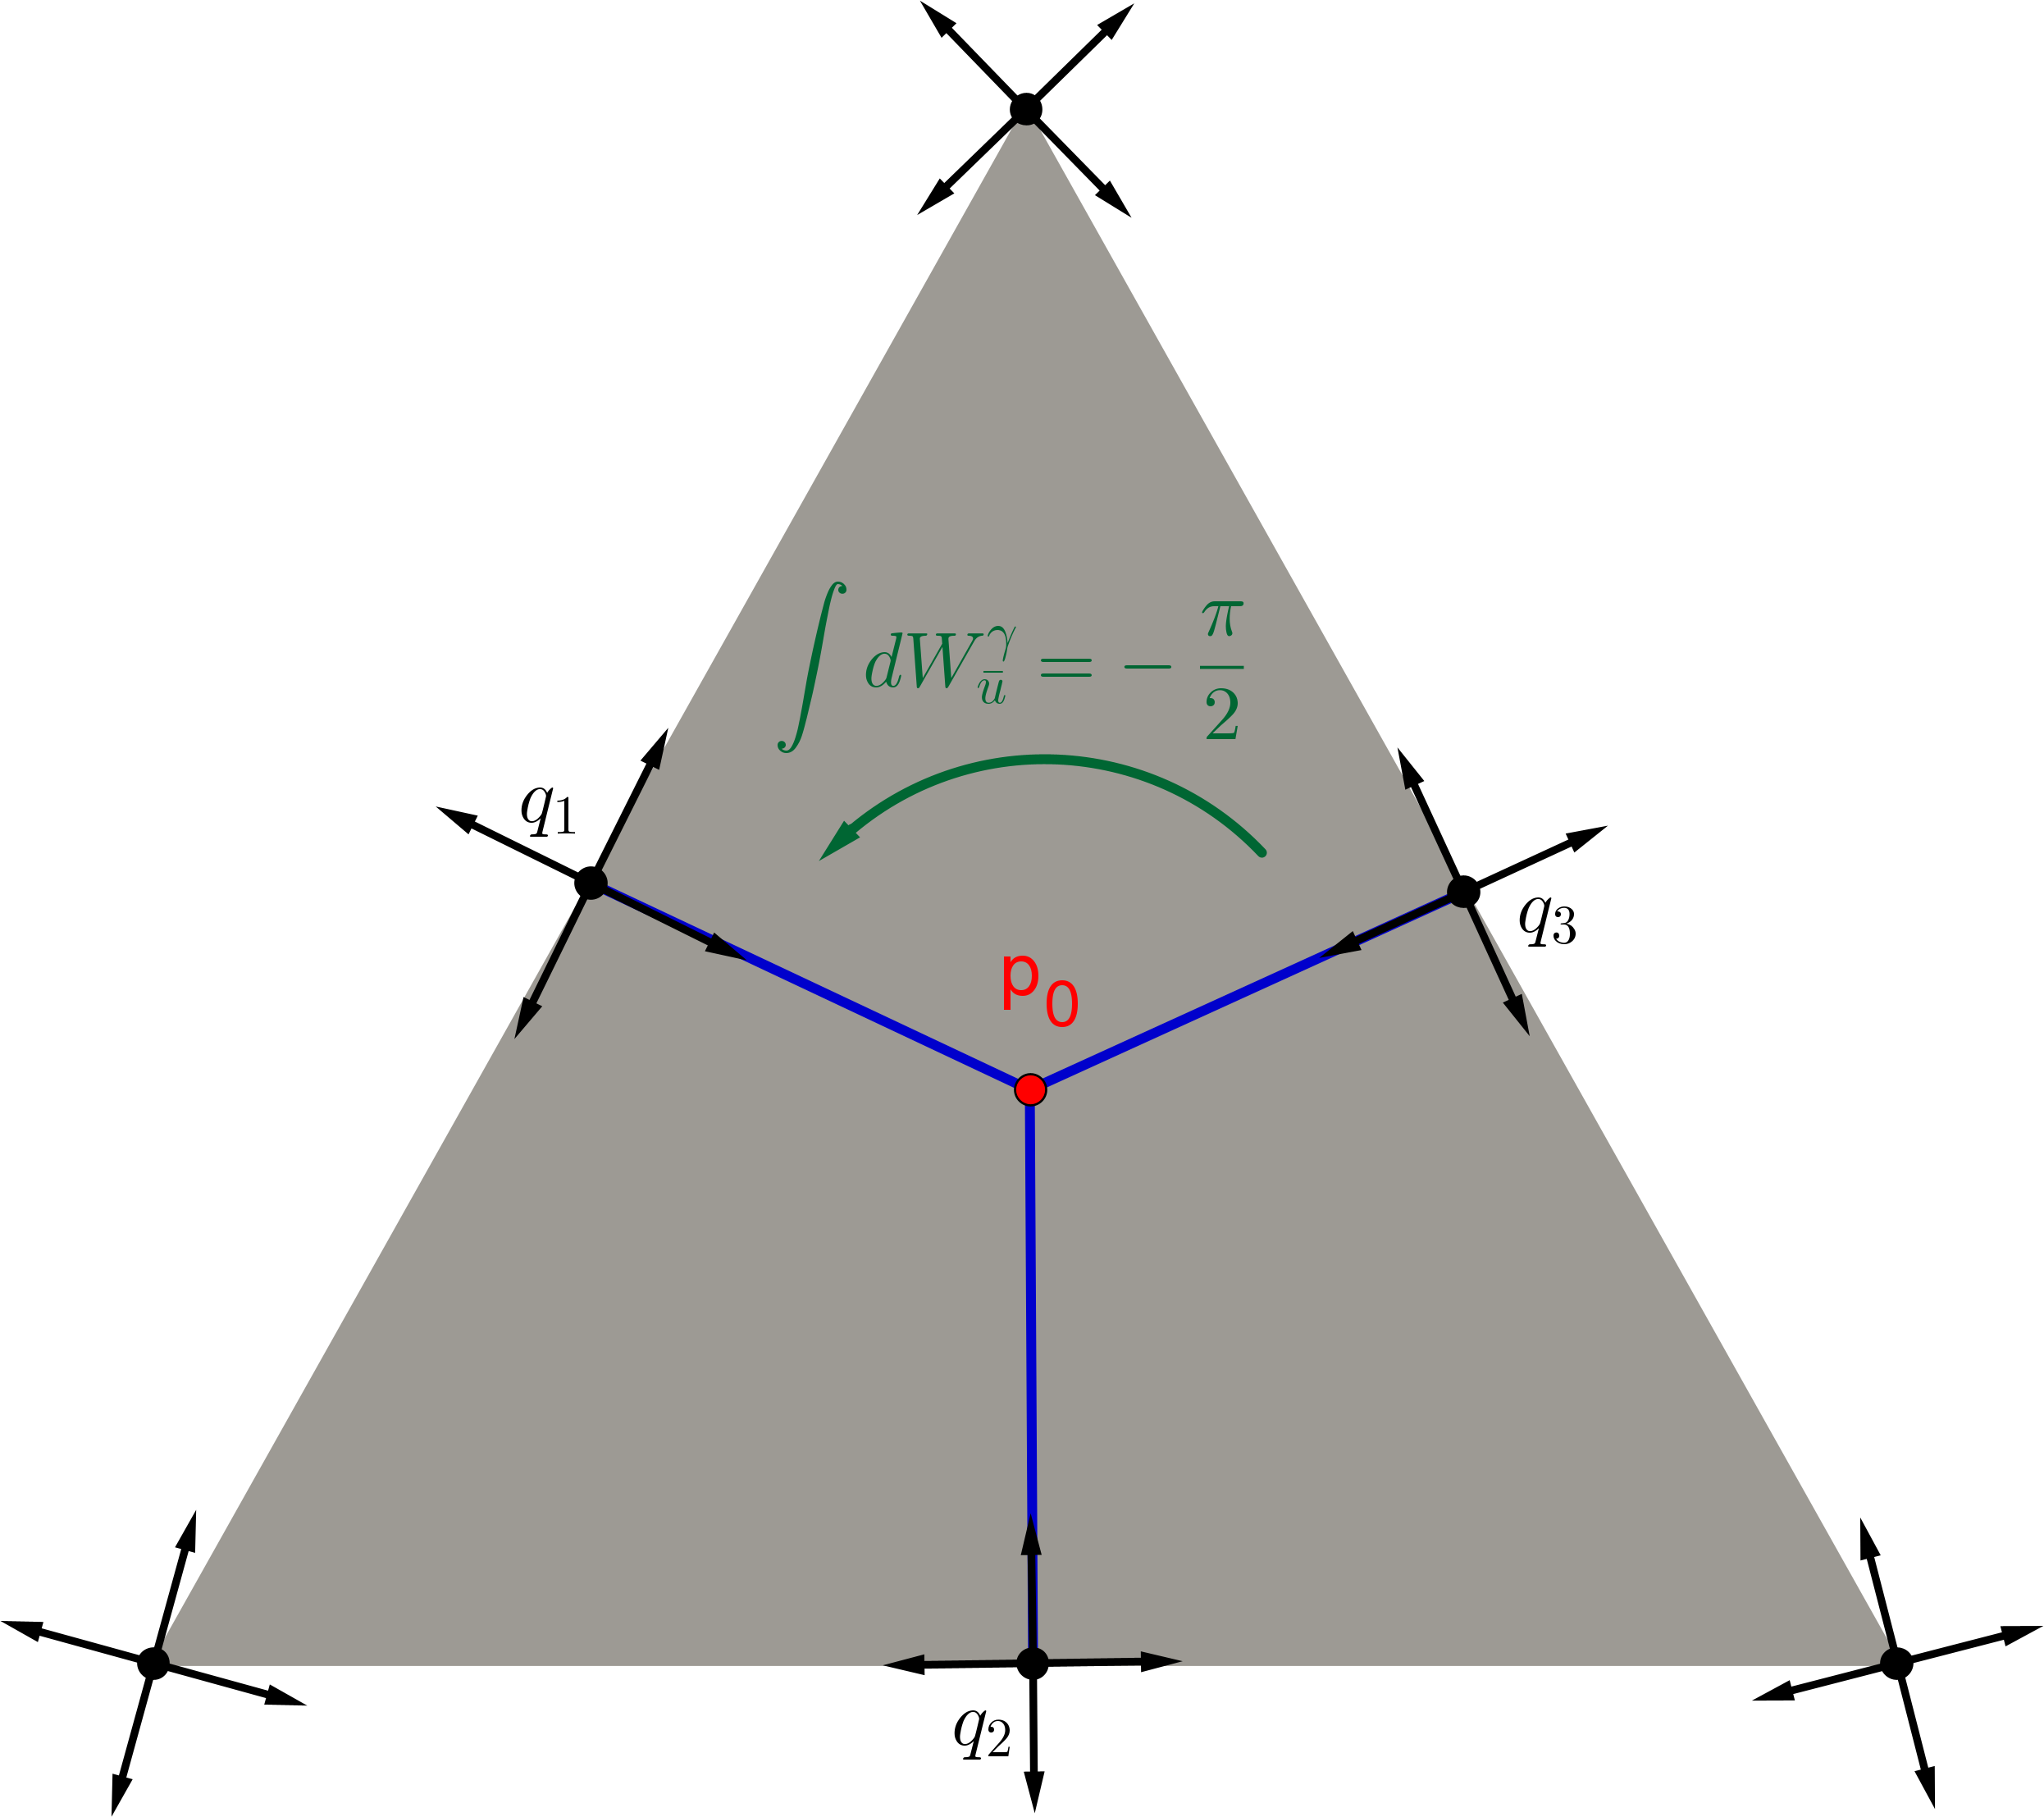
\includegraphics[scale=0.755]{images/triangle separatrices 3.png}
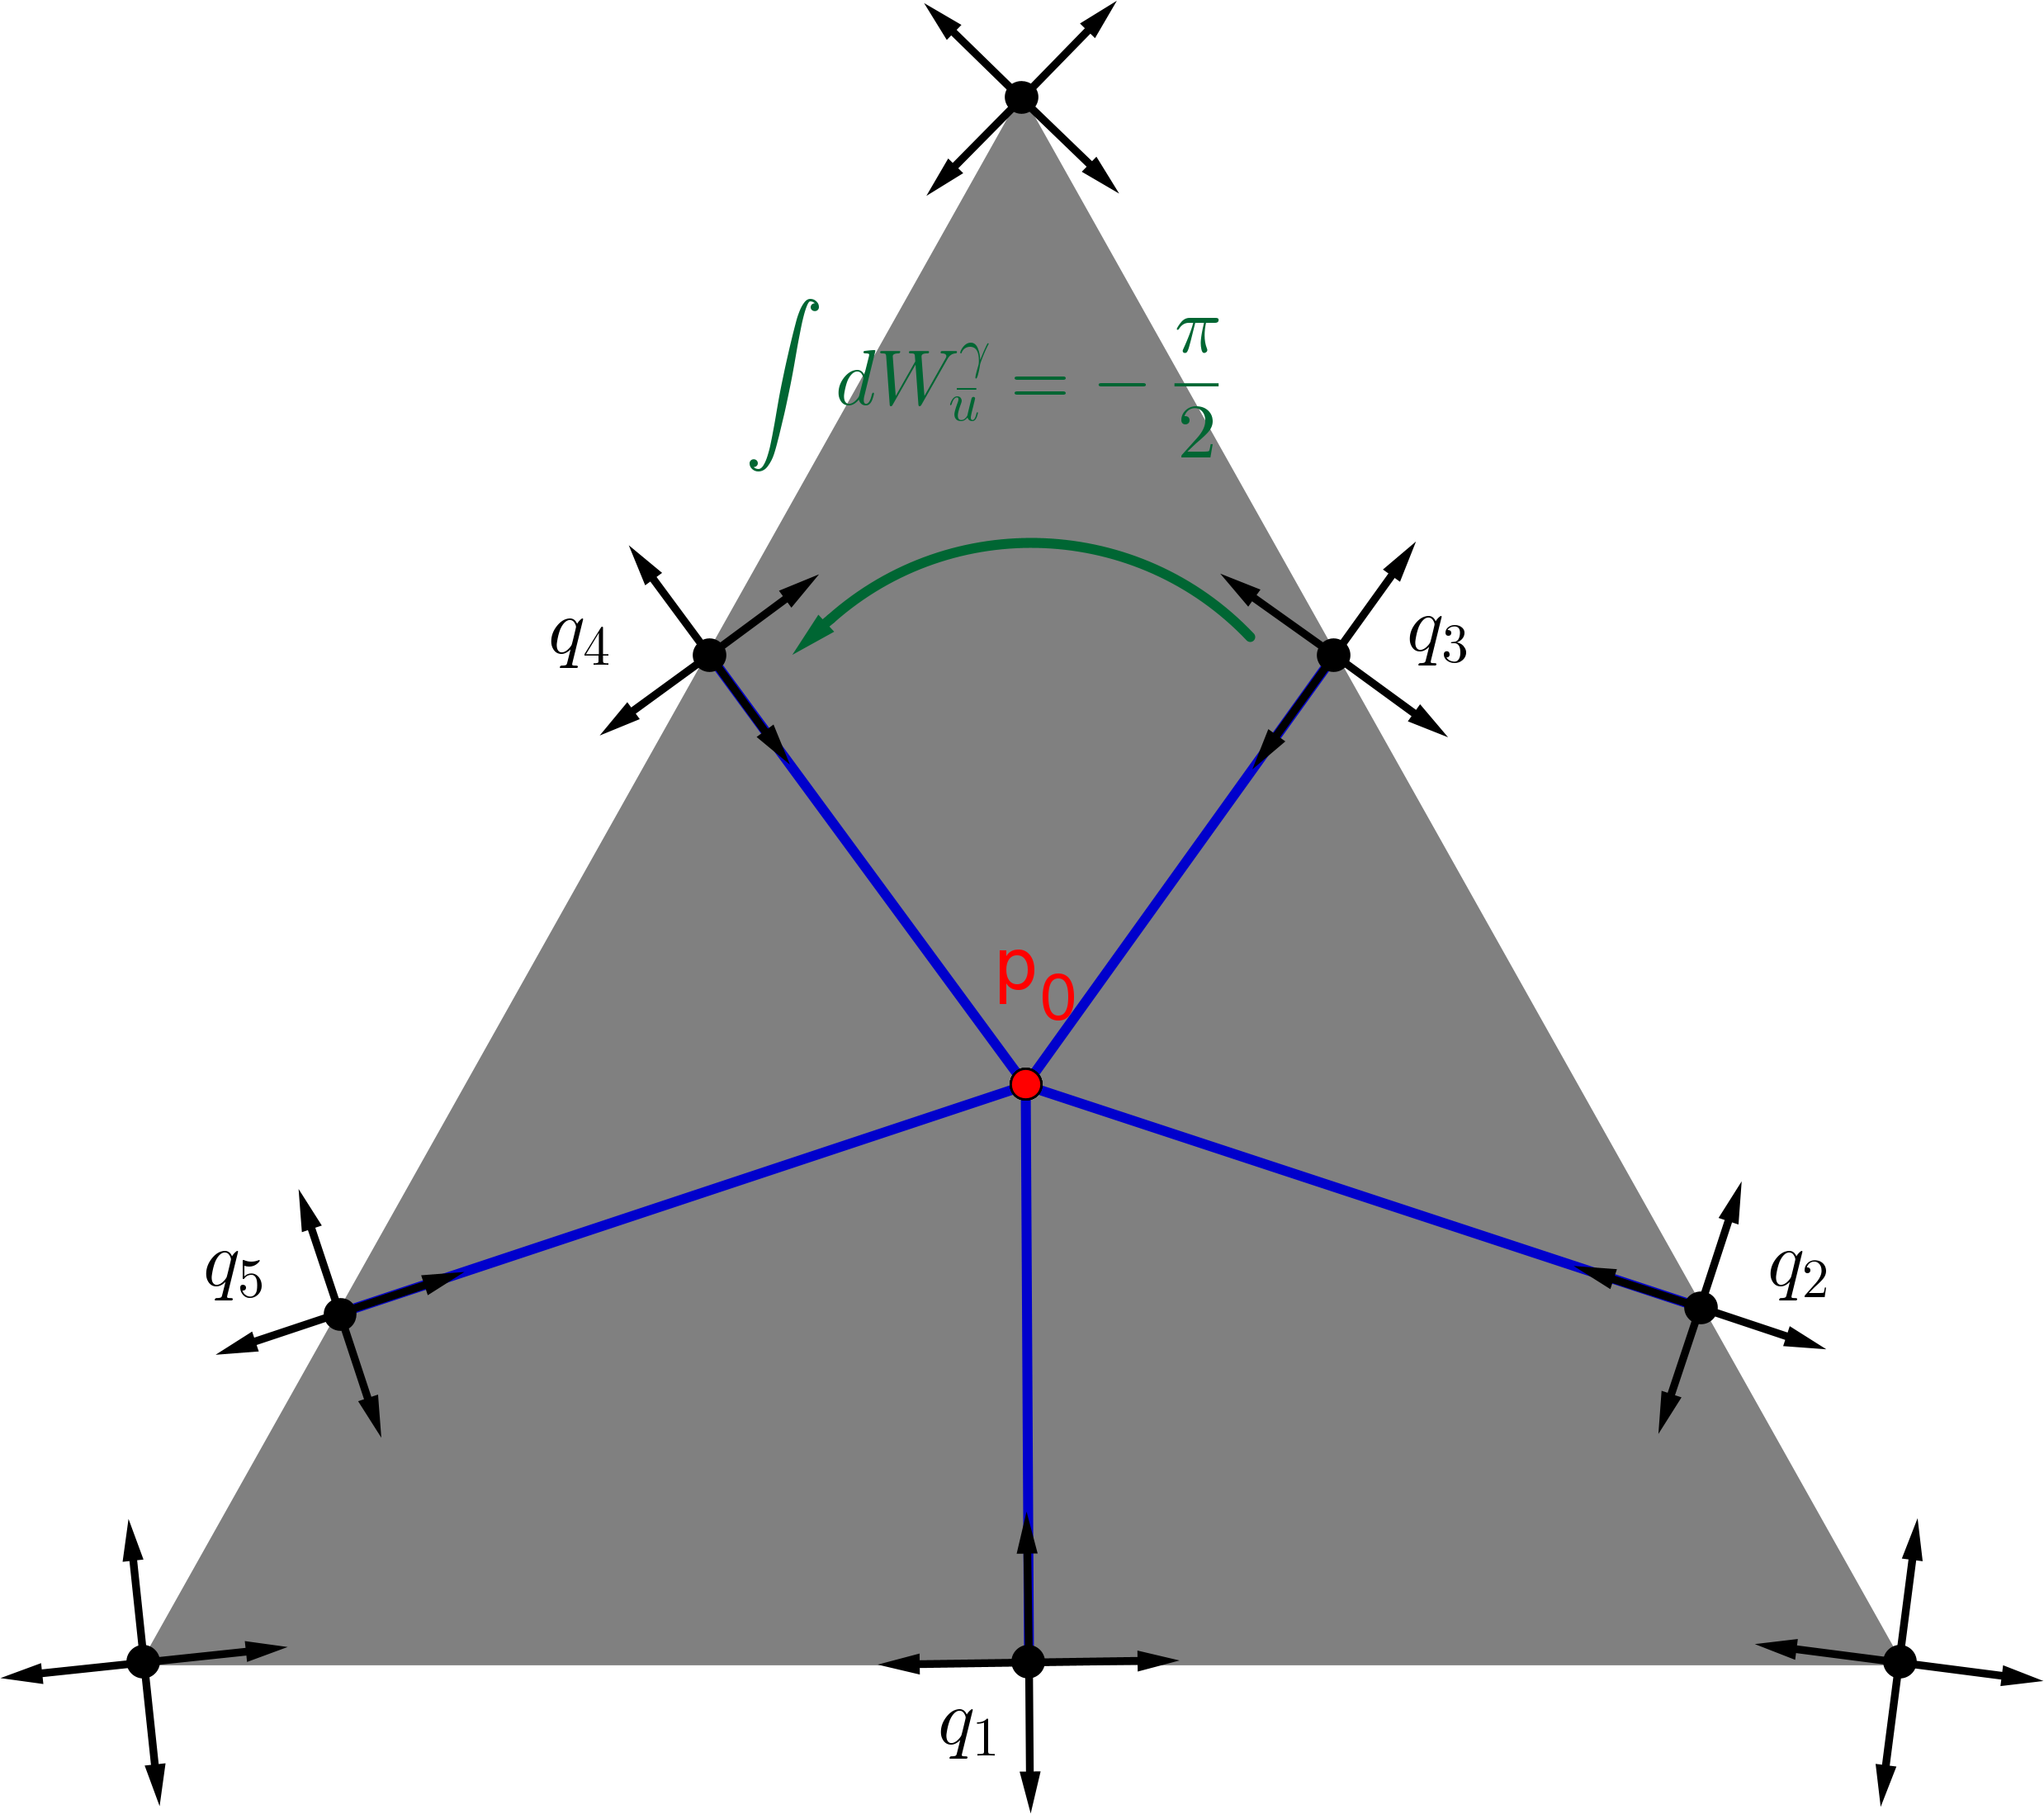
\includegraphics[scale=0.755]{images/triangle separatrices 5.png}
\caption{Illustration du maillage quadrilatéral d'un anneau à partir d'un champ de croix radial.}
\label{fig:init_streams_int}
\end{figure}

\begin{figure}[!h]
\centering
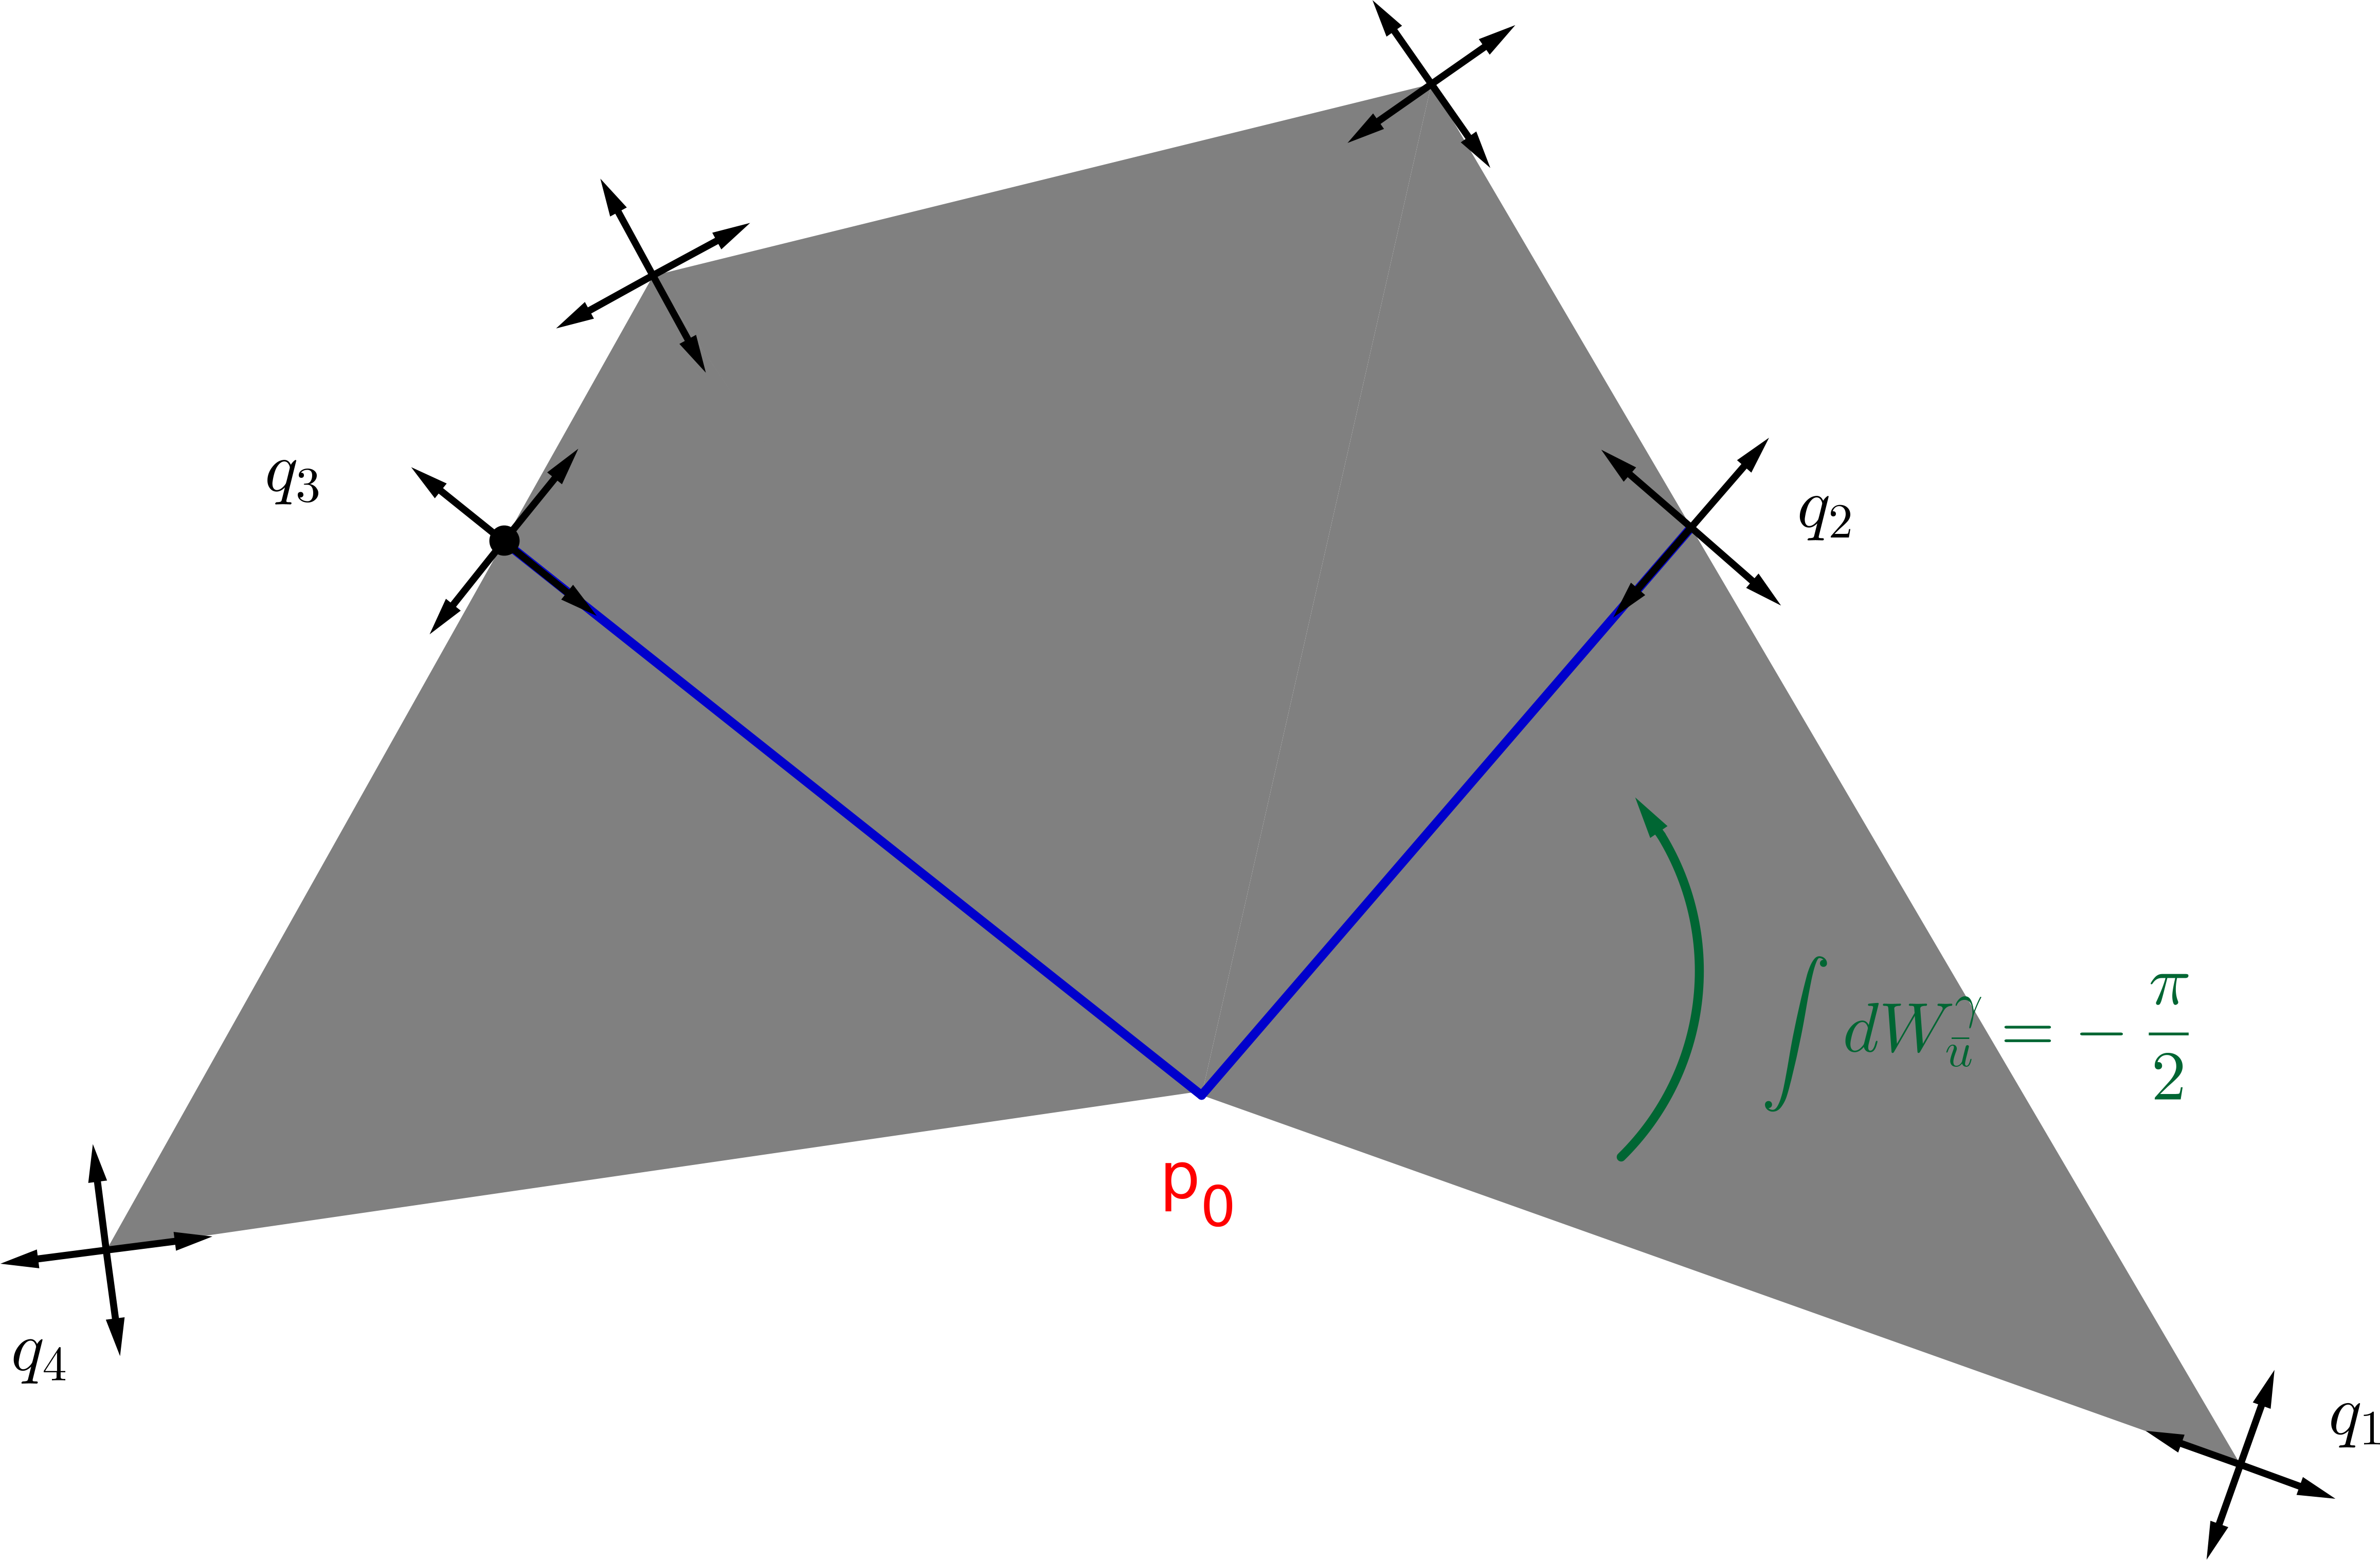
\includegraphics[scale=0.755]{images/triangle separatrices bord.png}
\caption{Illustration du maillage quadrilatéral d'un anneau à partir d'un champ de croix radial.}
\label{fig:init_streams_bord}
\end{figure}

\paragraph{Directions initiales et intégration:}

Soit $p_0\in\mathcal{S}_{\bar{u}_h}\backslash\partial\Omega_h$. Étant donné que $\bar{u}_h$ s'annule en $p_0$, notre première étape consiste à déterminer les orientations initiales des séparatrices. Les directions initiales des séparatrices émanant de $p_0$ sont données par les vecteurs $\overrightarrow{p_0q_i}$, $i\in\llbracket 1, N_s(p_0) \rrbracket$ où la suite de points $(q_i)_{i\in\llbracket 1, N_s(p_0)\rrbracket}\subset\partial T_{p_0}$ est construite de la manière suivante (voir figure \ref{fig:init_streams_int}):\\
\begin{itemize}
    \item[$\bullet$] le premier point $q_1$ est tout point de $\partial T_{p_0}$ tel que $\overrightarrow{p_0q_1}.\|\overrightarrow{p_0q_1}\|^{-1}\in\bar{u}_h(q_1)$\\
    \item[$\bullet$] soit $t_1\in[0, 1]$ tel que $\gamma(t_1)=q_1$. Pour tout $i\in\llbracket 2, N_s(p_0)\rrbracket$, on a:
    $$
    q_i=\gamma(t_i)\mbox{ avec }\int_{t_{i-1}}^{t_i}dW_{p_0}^\gamma=-\frac{\pi}{2},
    $$
    où $\gamma$ est une paramétrisation de $\partial T_{p_0}$ sur $[0, 1]$ dans le sens positif et la fonction $W^\gamma_{p_0}$ est donné pour tout $t\in[0, 1]$ par:
    $$
    W_{p_0}^\gamma(t)=\theta^\gamma_{\bar{u}_h}(t)-\arg \overrightarrow{p_0\gamma(t)}.
    $$
\end{itemize}

Le principe demeure inchangé lorsque $p_0$ est un point singulier de bord ($p_0\in\mathcal{S}_{\bar{u}_h}\cap\partial\Omega_h$) (voir la figure \ref{fig:init_streams_bord}). Dans ce cas, le premier point $q_1$ est unique et correspond à $\gamma(0)$ où $\gamma$ est une paramétrisation sur $[0, 1]$ de $\partial T{p_0}\backslash\partial\Omega_h$ dans le sens positif. Une fois les orientations initiales déterminées, l'intégration d'une séparatrice correspond exactement au processus d'intégration d'une ligne de champ tel que décrit dans la section \ref{subsec:pt_sing_ind_lign_champ}.

\begin{figure}[h!]
\centering
\begin{subfigure}[b]{0.7\textwidth}
    \centering
    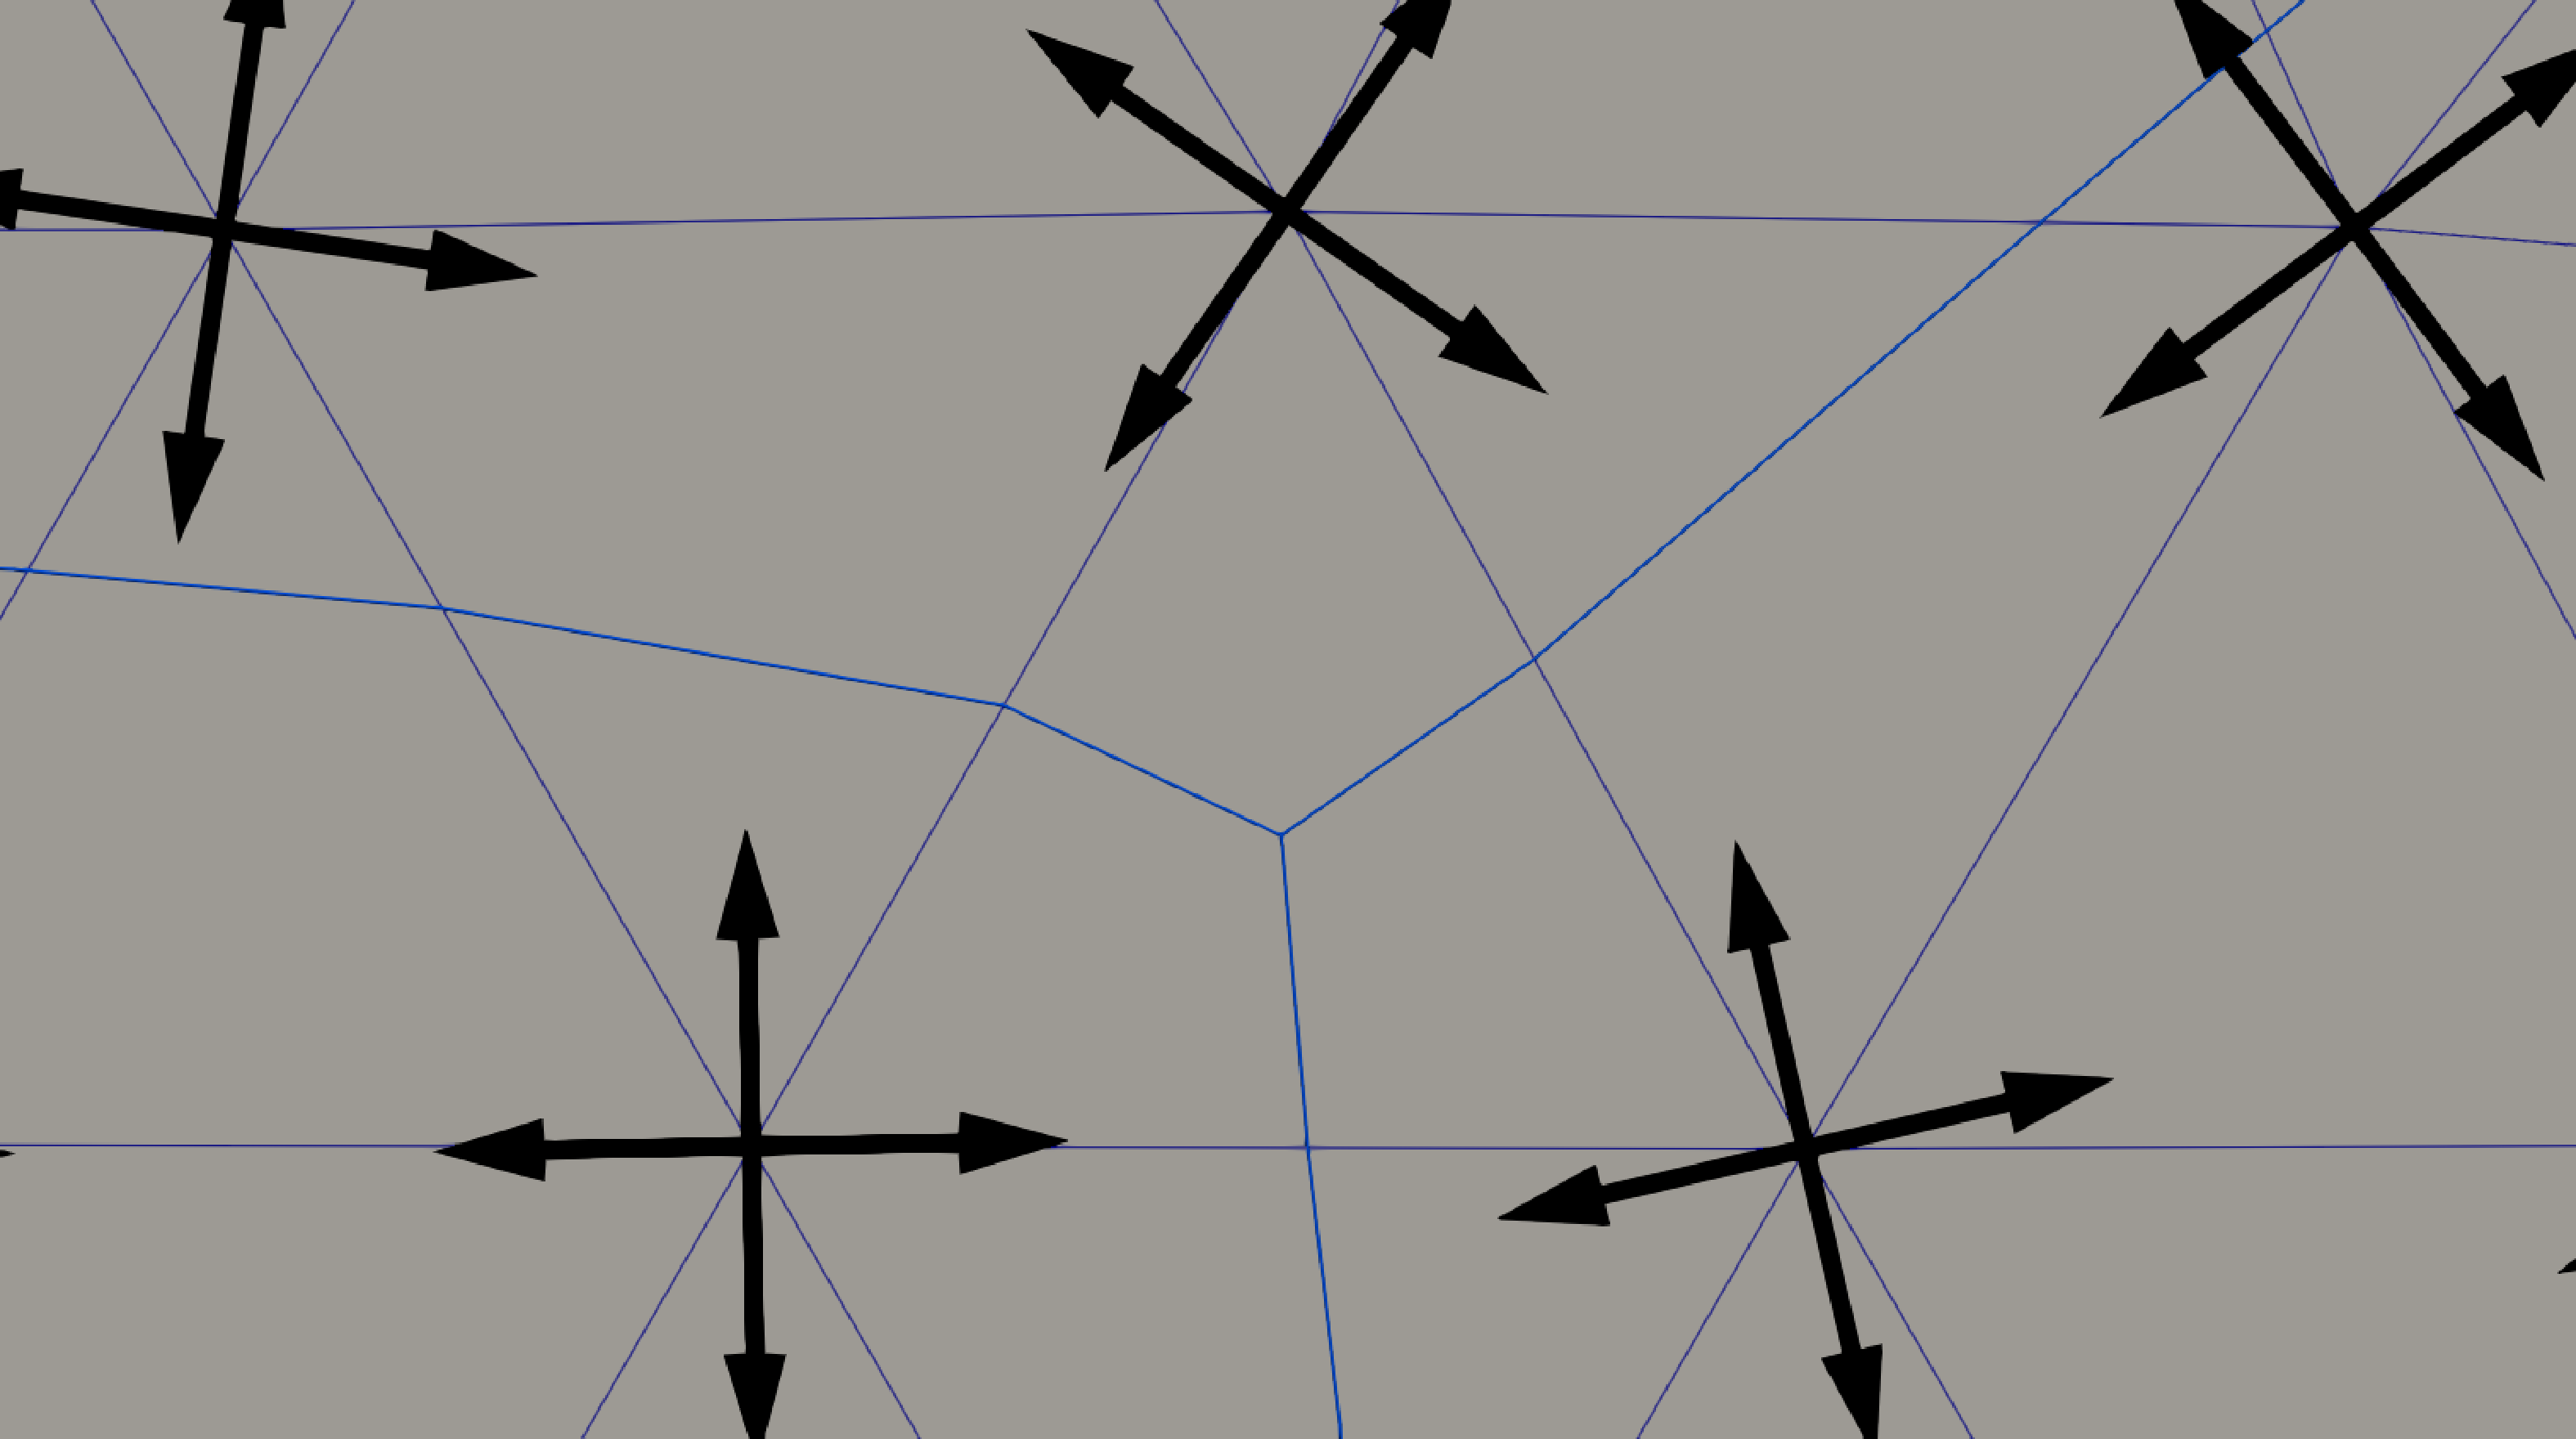
\includegraphics[width=\textwidth]{images/depart_sepa_1.pdf}
    \caption{Répartition uniforme des différences angulaires entre les directions de sortie.}
\end{subfigure}
\\[0.5cm]
\begin{subfigure}[b]{0.7\textwidth}
    \centering
    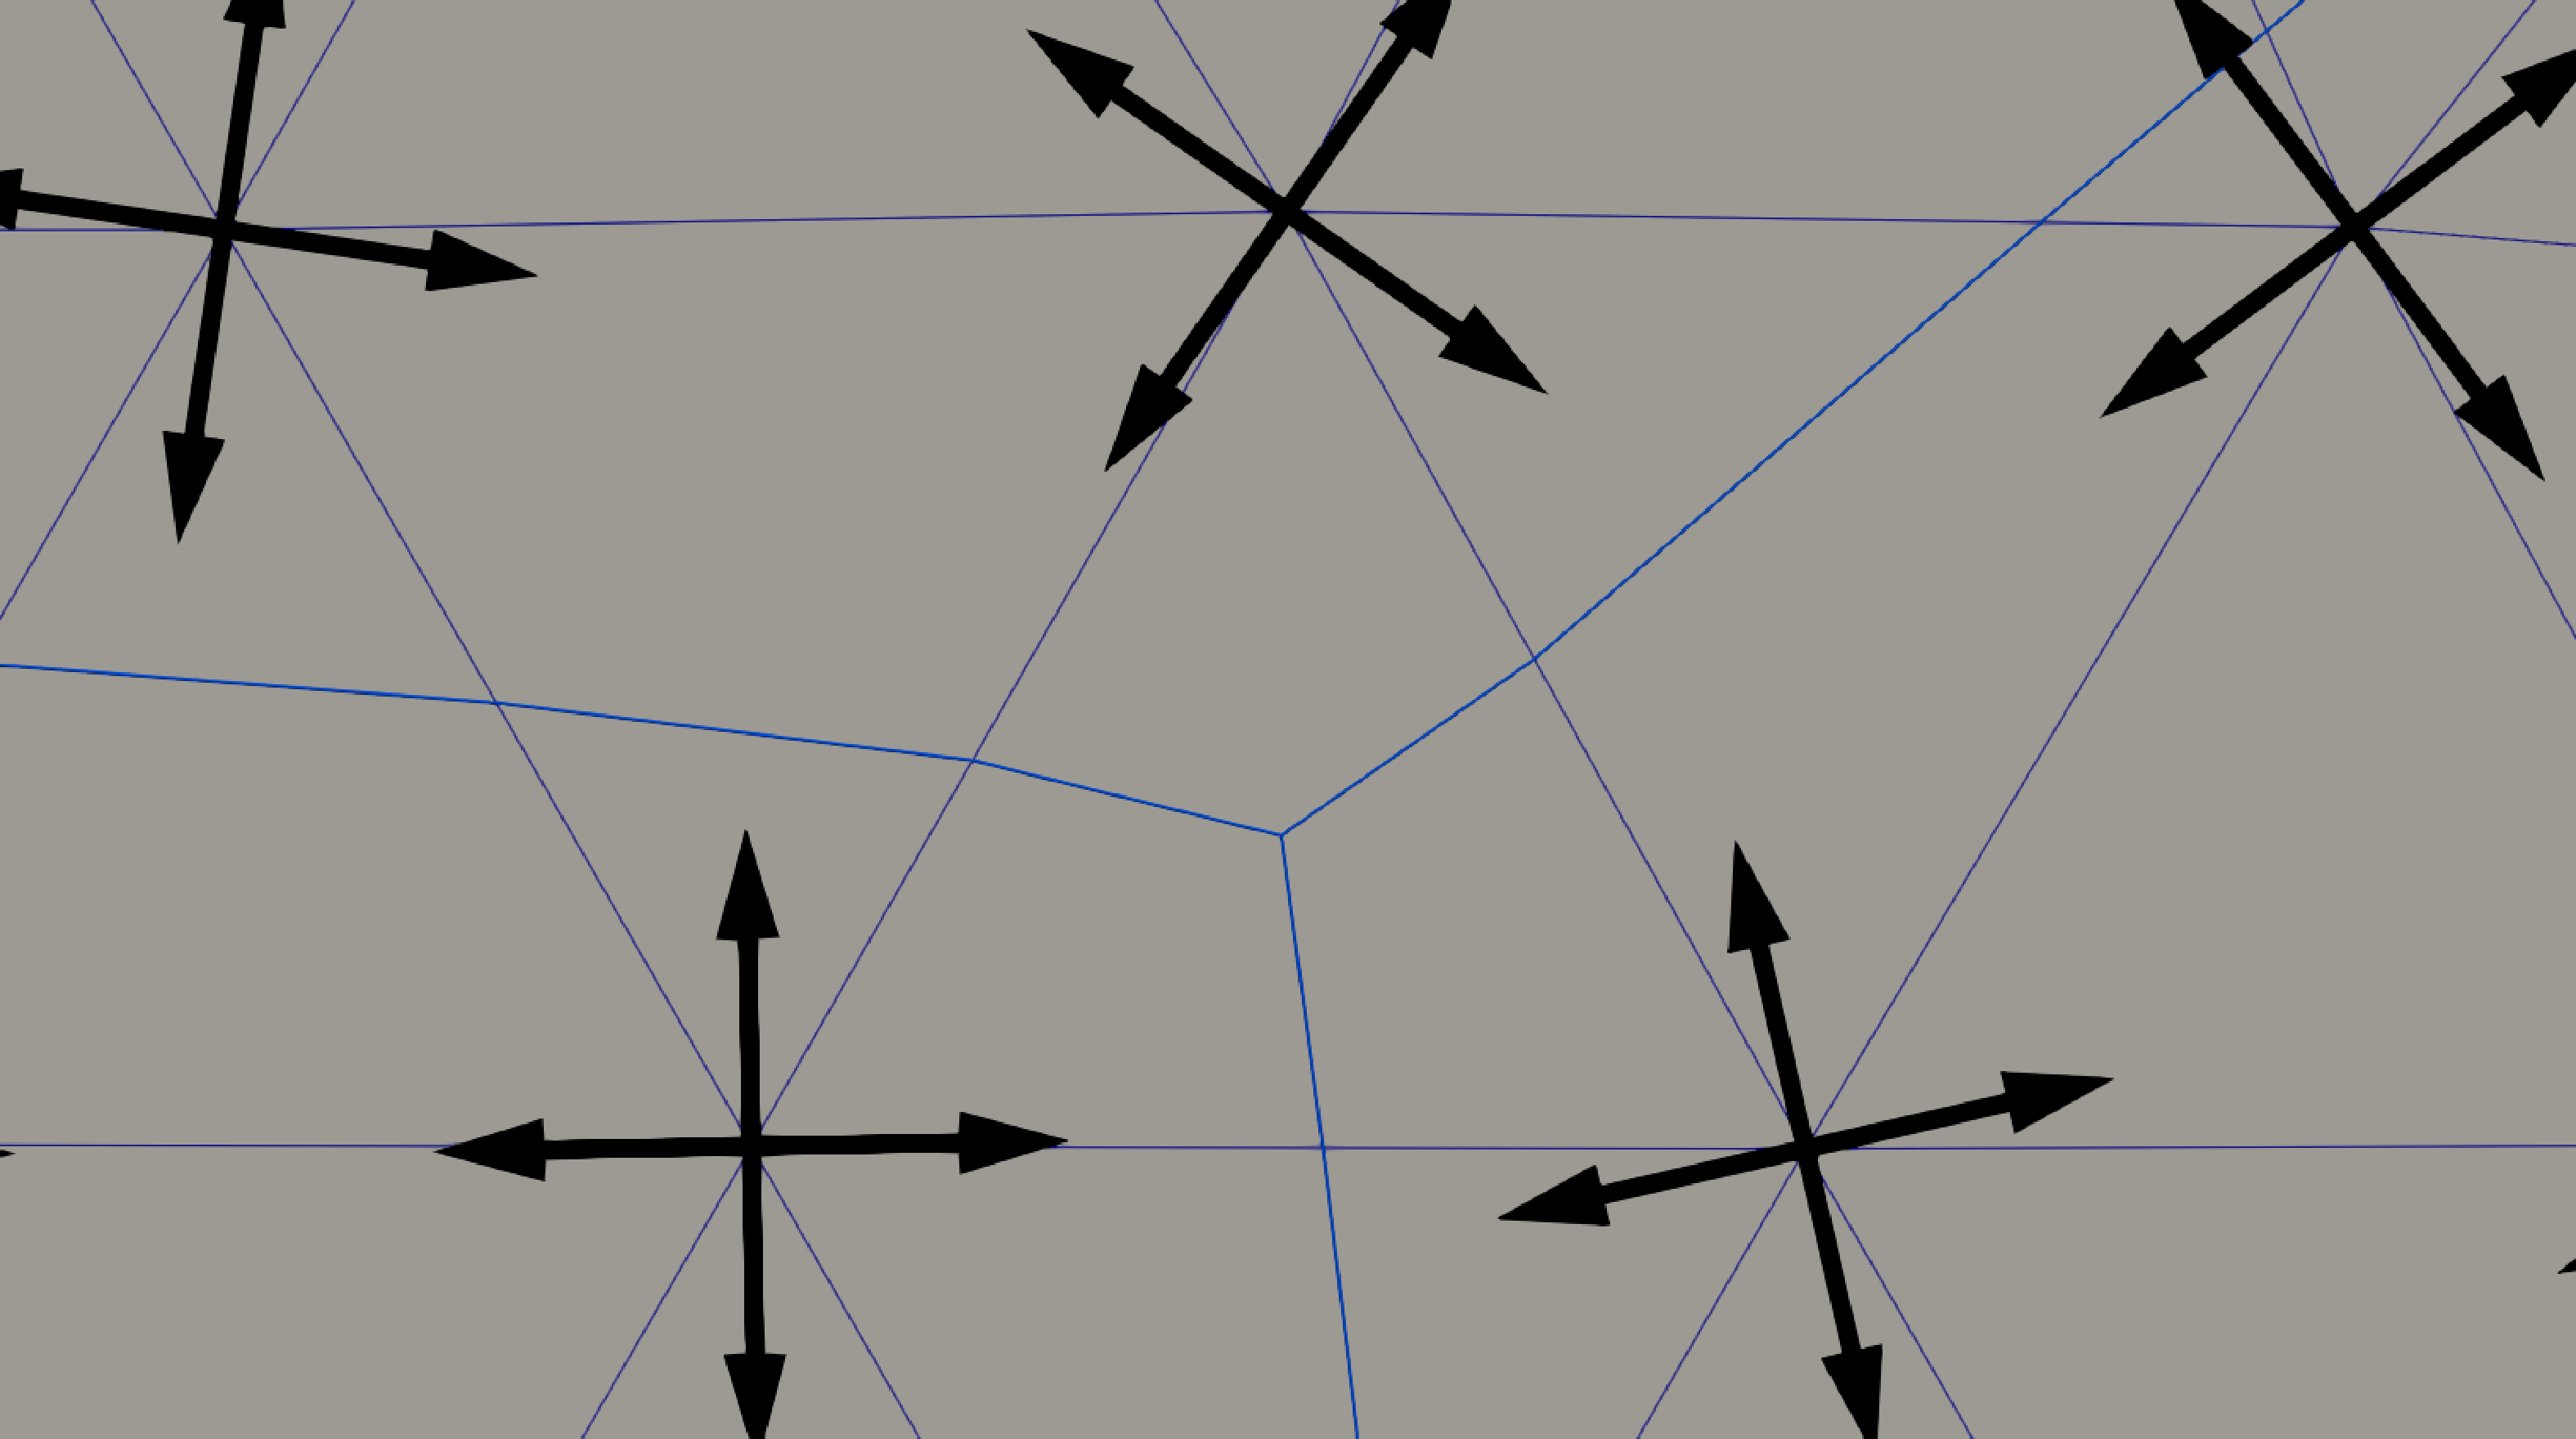
\includegraphics[width=\textwidth]{images/depart_sepa_2.pdf}
    \caption{Calcul des directions de sortie à l'aide de notre méthode.}
\end{subfigure}
\caption{Illustration des directions de sortie des séparatrices d'un point singulier d'indice $1/4$, utilisant deux méthodes distinctes.}
\label{fig:first_dir}
\end{figure}

\begin{remark}
Dans la littérature, les directions initiales sont souvent calculées de manière uniforme autour du point singulier. Par exemple, pour un point singulier d'indice $1/4$, les directions initiales des trois séparatrices sont espacées d'une différence angulaire de $2\pi/3$ les unes des autres. Nous observons ainsi que la méthode d'initialisation que nous proposons ci-dessus est plus précise et fournit de meilleurs résultats (voir la figure \ref{fig:first_dir}).
\end{remark}




\paragraph{Traversé d'un triangle singulier:}

\begin{figure}[!h]
\centering
\begin{subfigure}[b]{0.495\textwidth}
    \centering
    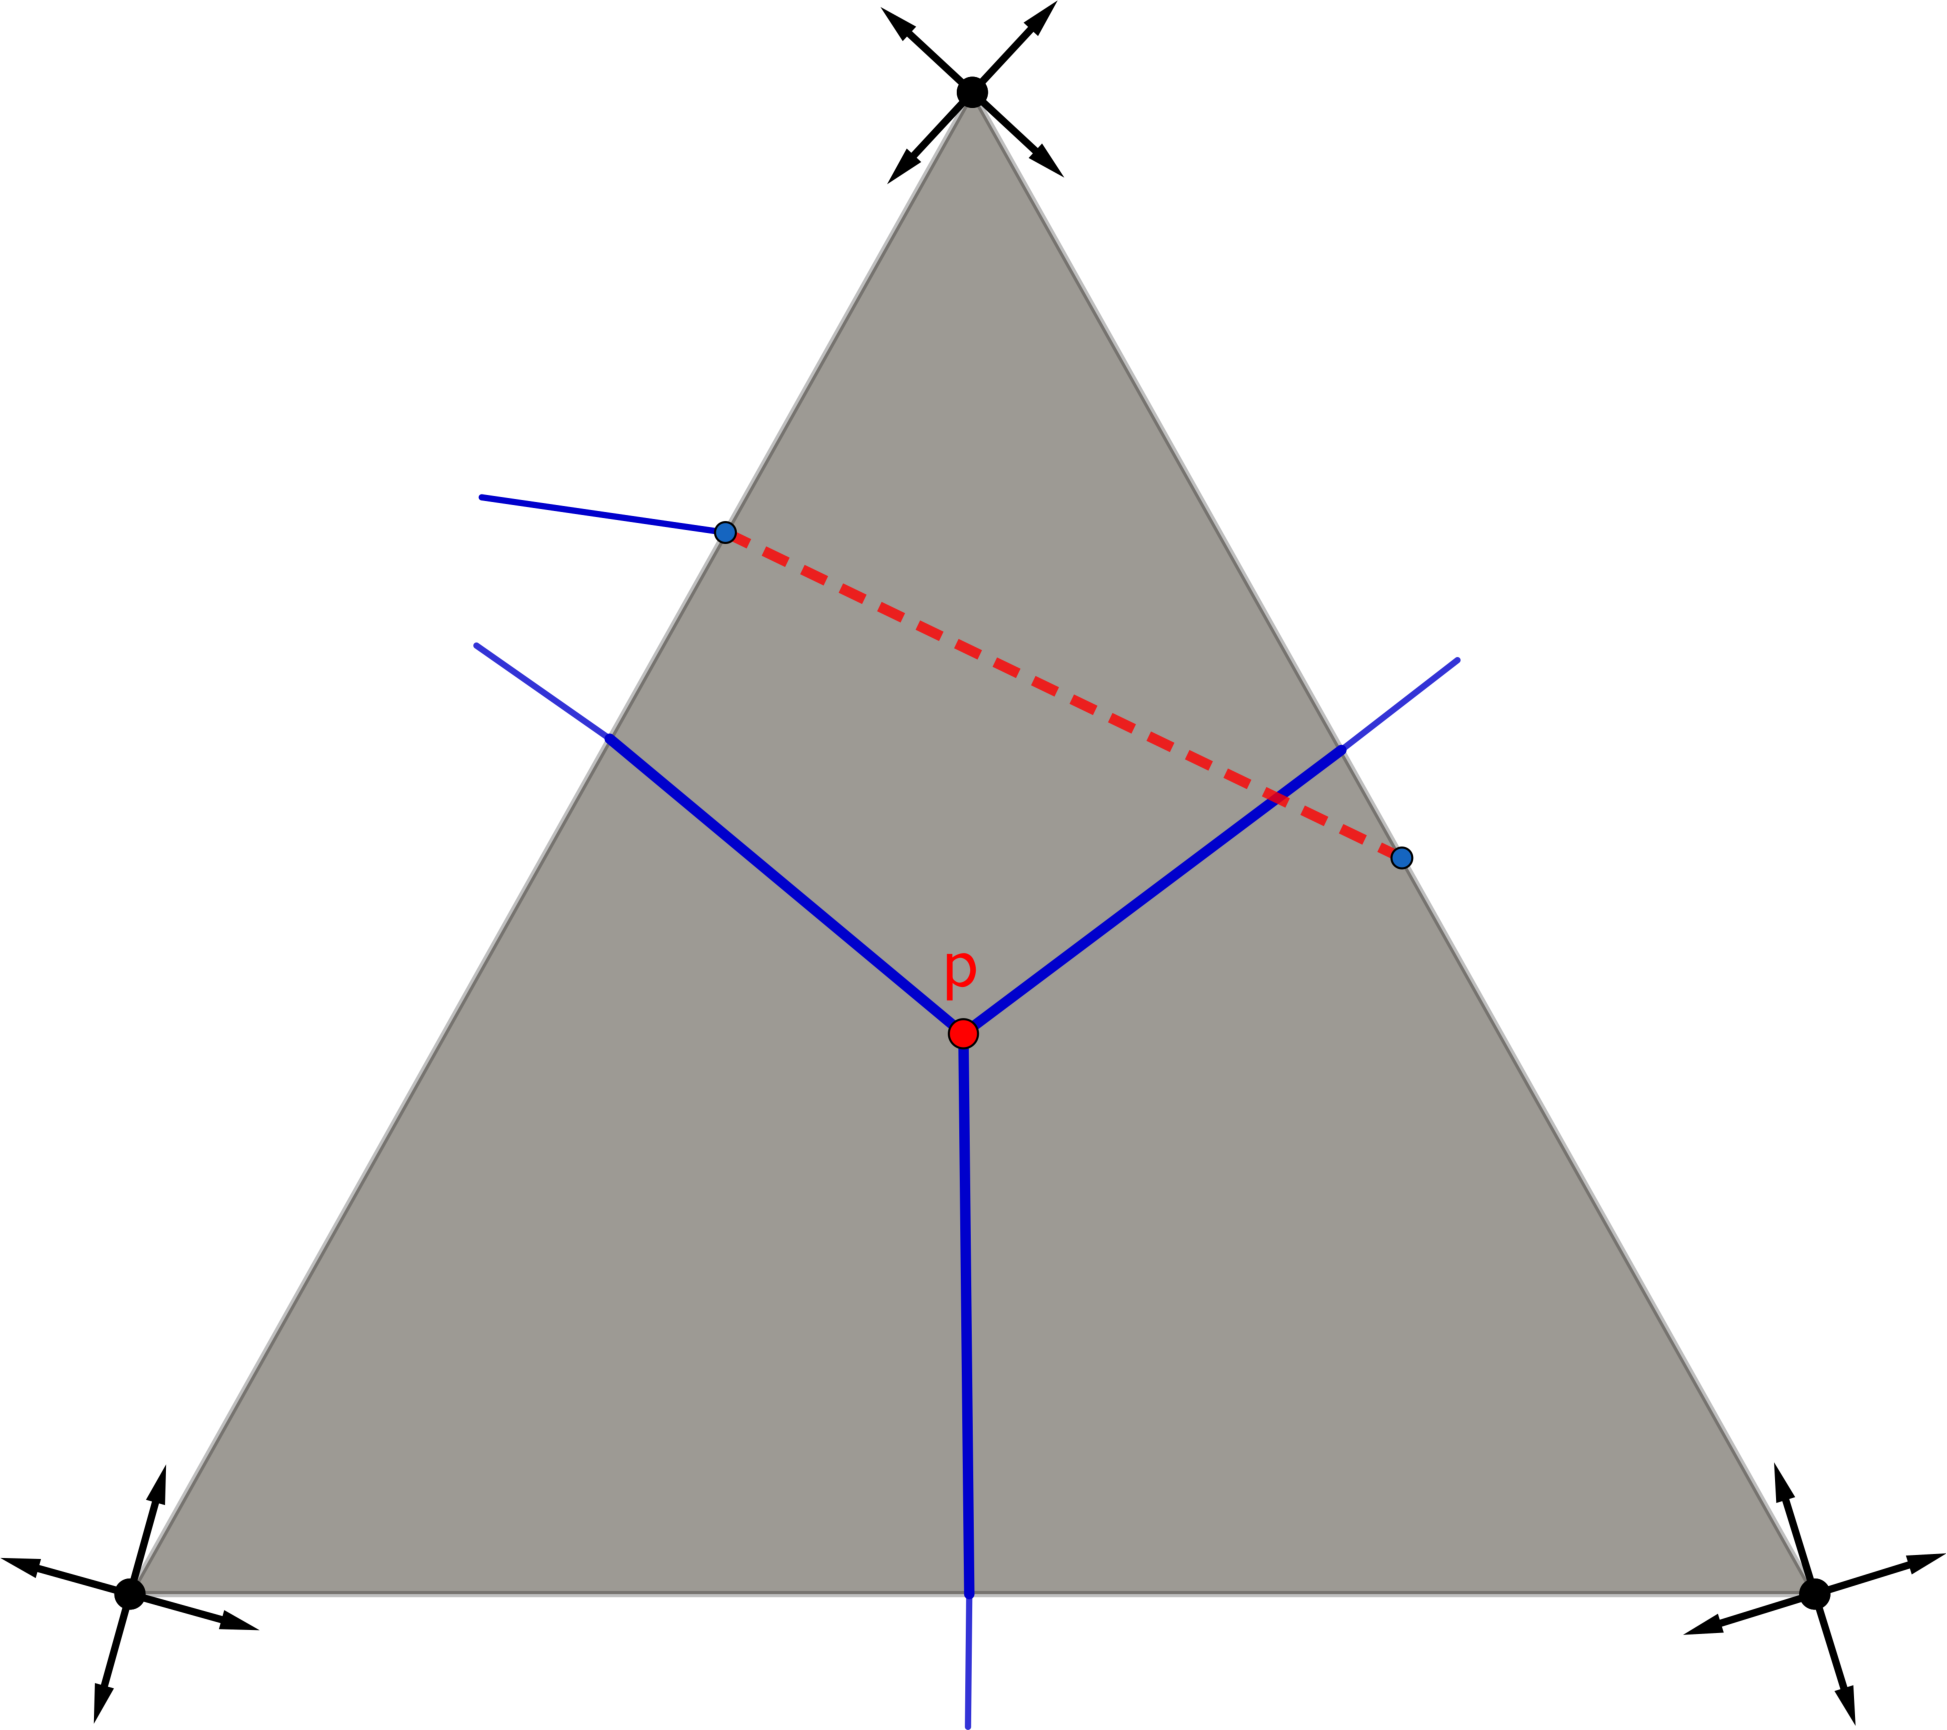
\includegraphics[width=\textwidth]{images/draw_streams_sing_1.pdf}
    \caption{\'Echec d'intégration d'une séparatrice dans un triangle singulier.}
    \label{fig:draw_streams_sing_1}
\end{subfigure}
\hfill
\begin{subfigure}[b]{0.495\textwidth}
    \centering
    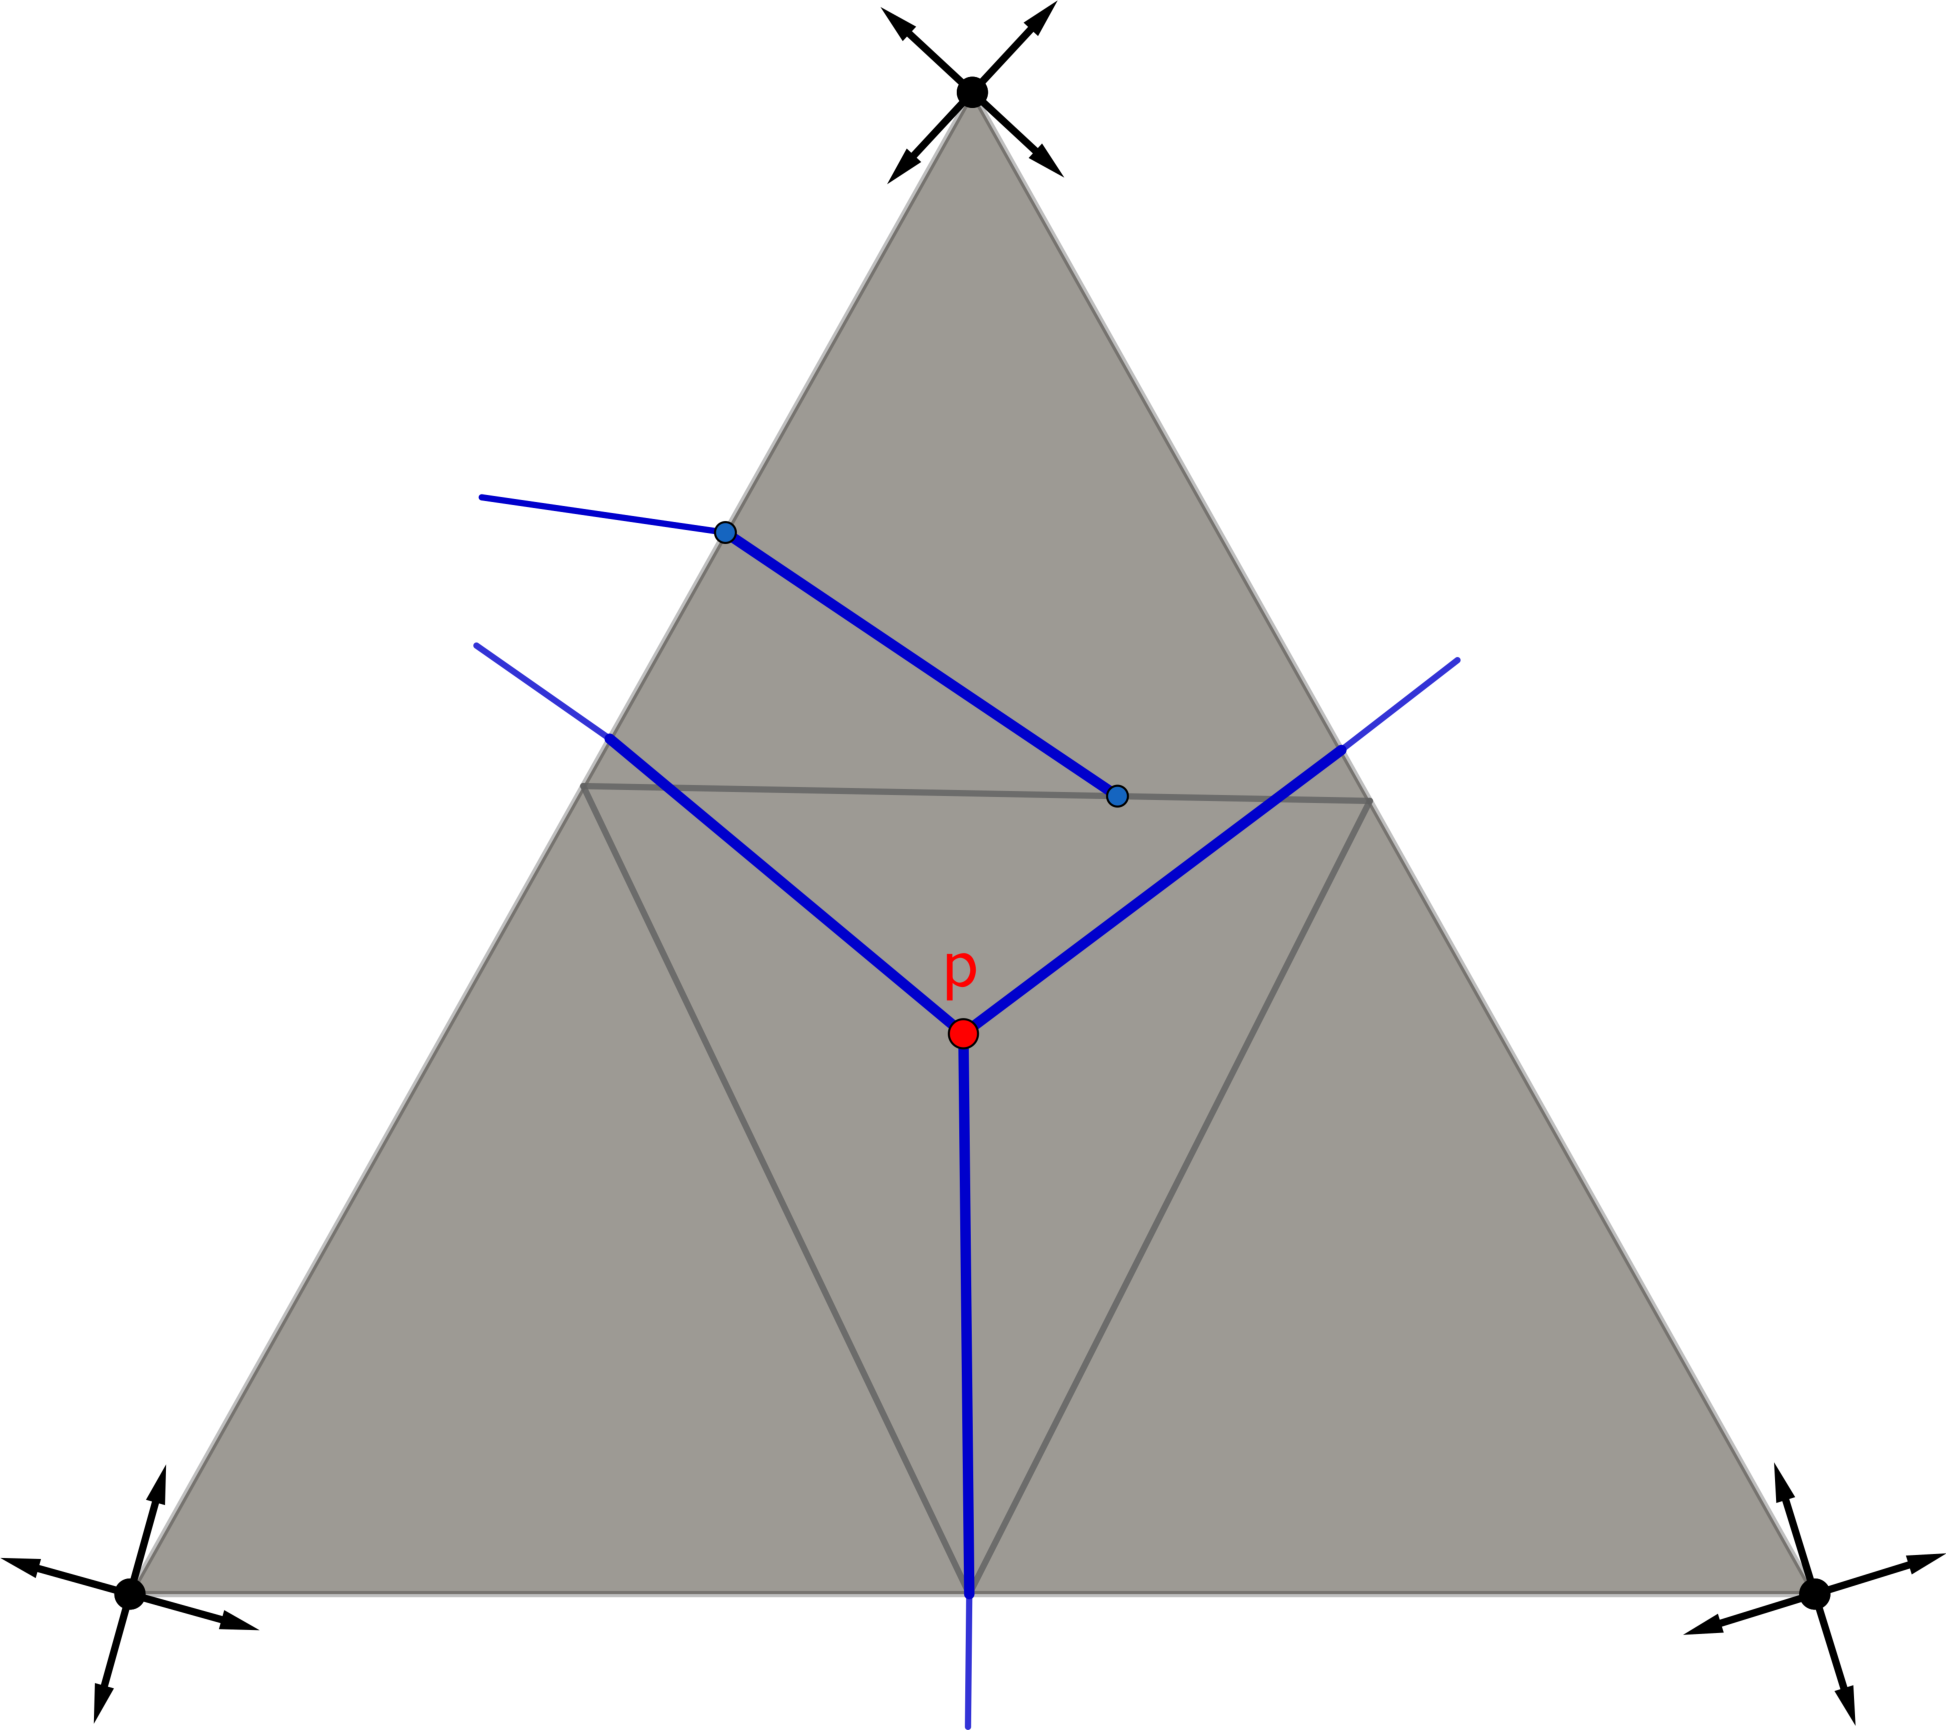
\includegraphics[width=\textwidth]{images/draw_streams_sing_2.pdf}
    \caption{Processus d'intégration d'une séparatice dans un triangle singulier: étape 1.}
    \label{fig:draw_streams_sing_2}
\end{subfigure}
\\[0.8cm]
\begin{subfigure}[b]{0.495\textwidth}
    \centering
    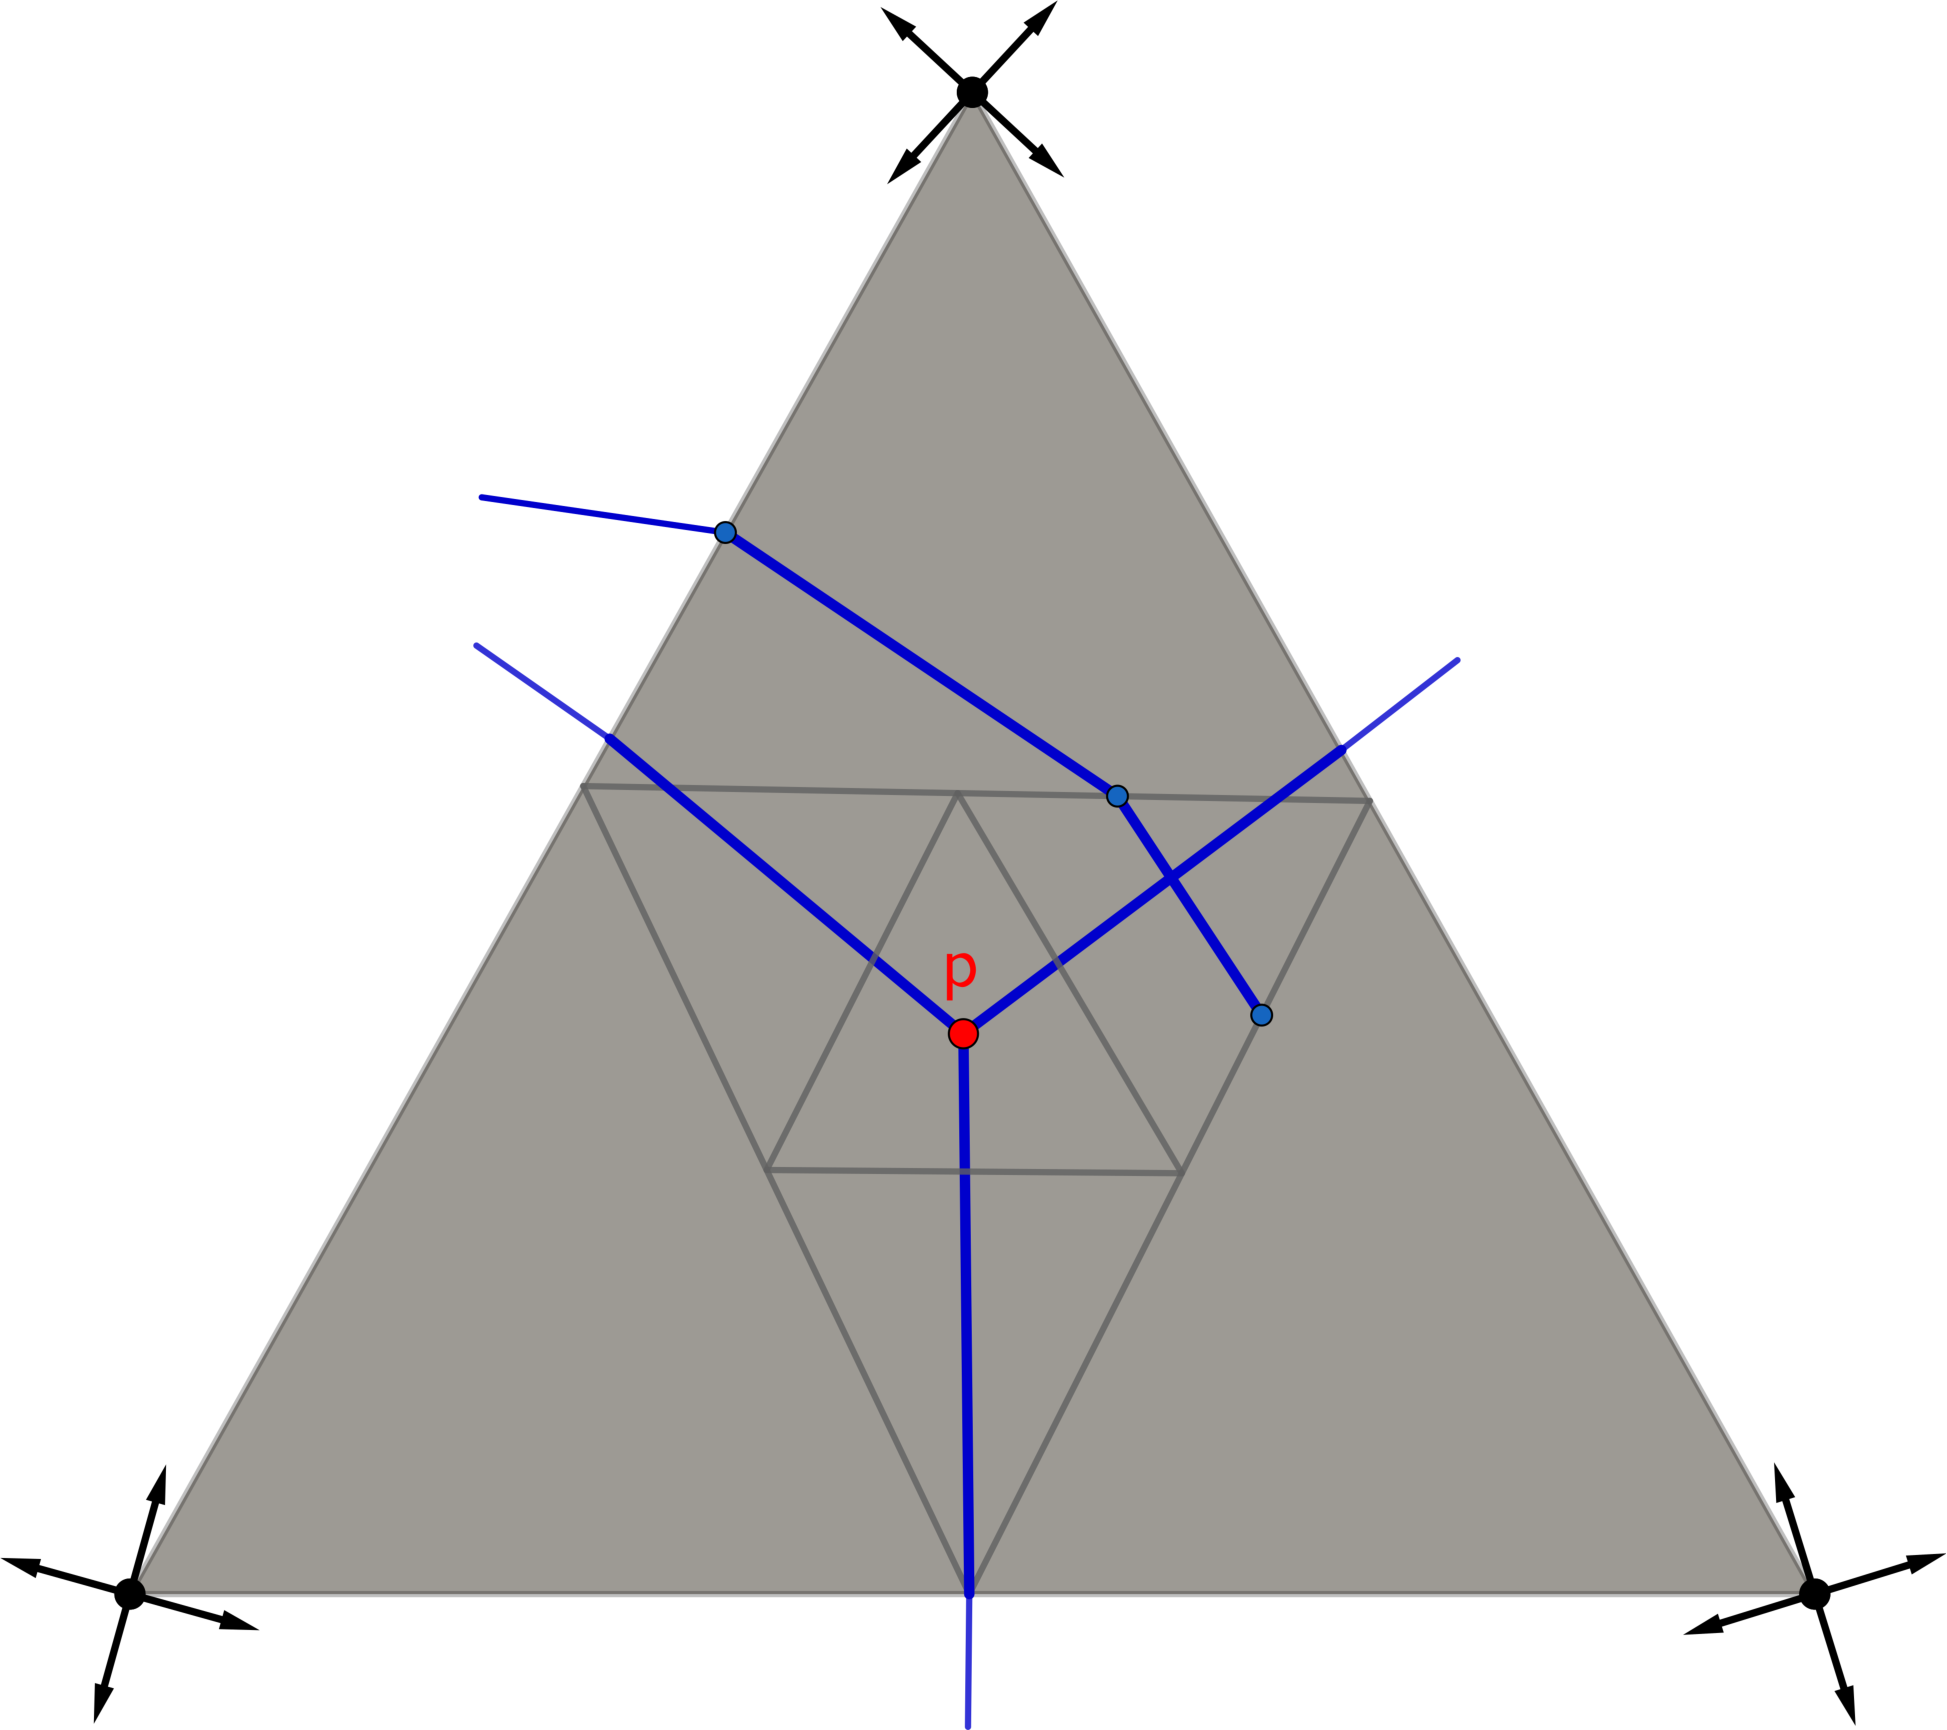
\includegraphics[width=\textwidth]{images/draw_streams_sing_3.pdf}
    \caption{Processus d'intégration d'une séparatice dans un triangle singulier: étape 2.}
    \label{fig:draw_streams_sing_3}
\end{subfigure}
\hfill
\begin{subfigure}[b]{0.495\textwidth}
    \centering
    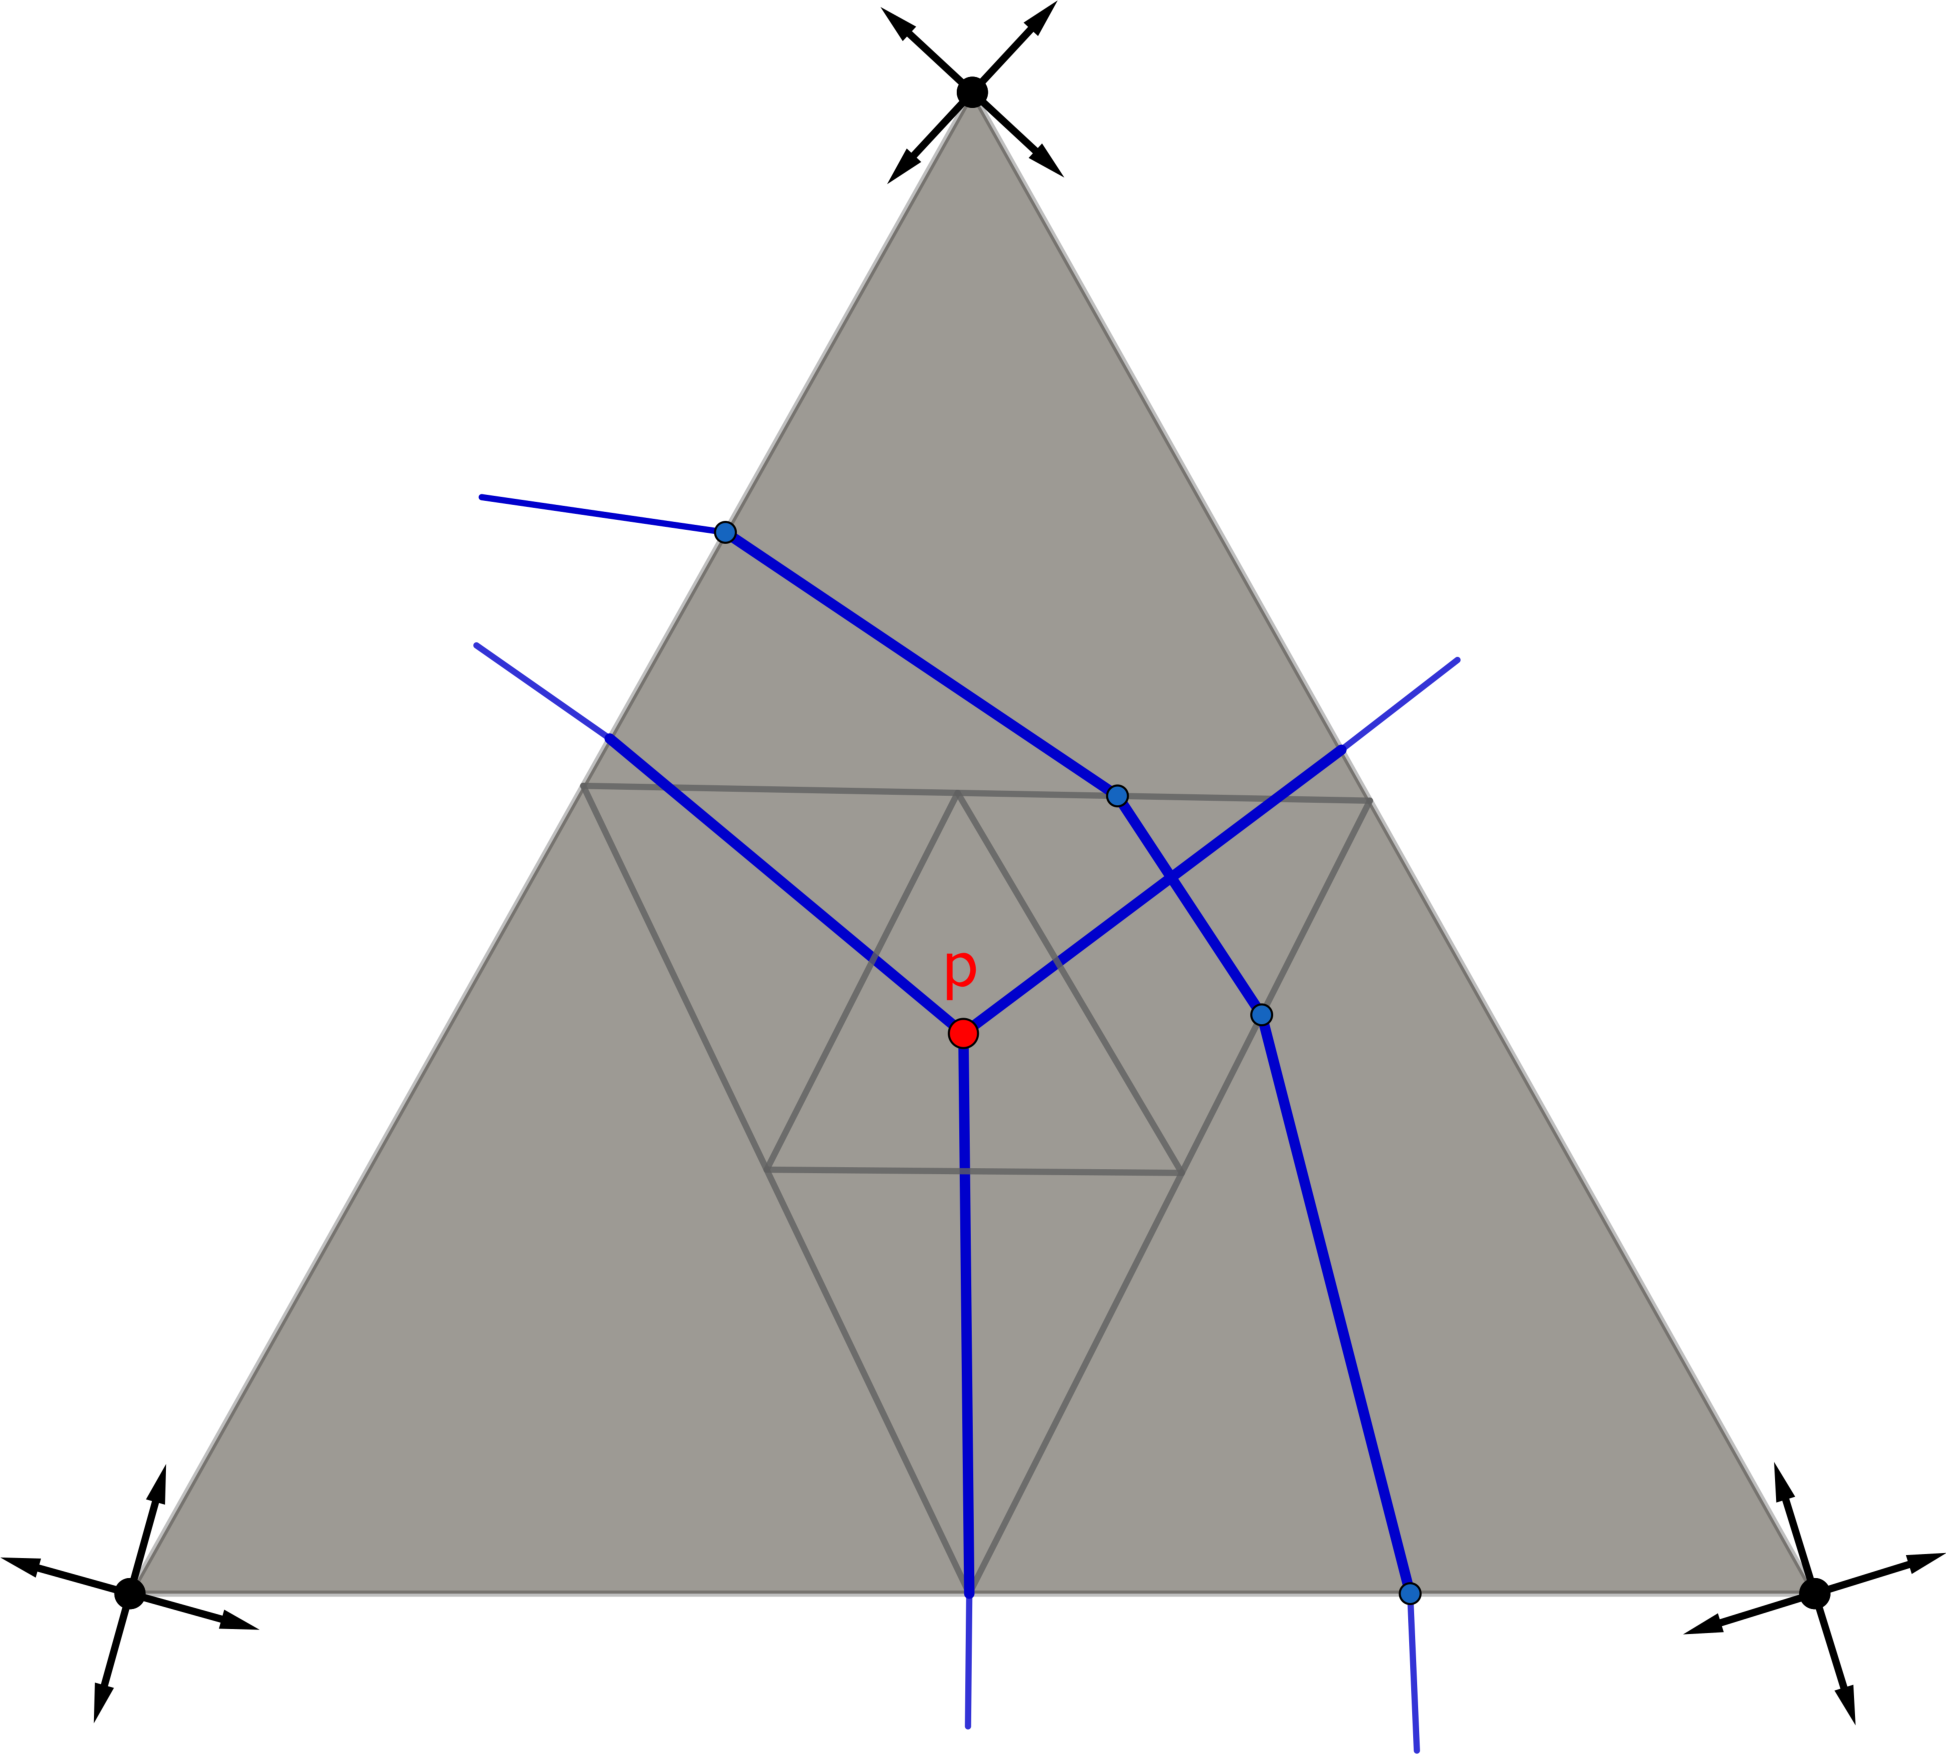
\includegraphics[width=\textwidth]{images/draw_streams_sing_4.pdf}
    \caption{Processus d'intégration d'une séparatice dans un triangle singulier: étape 3.}
    \label{fig:draw_streams_sing_4}
\end{subfigure}
\caption{Illustration de l'intégration d'une séparatice dans un triangle singulier.}
\label{fig:draw_streams_sing}
\end{figure}

\begin{figure}[!h]
\centering
\begin{subfigure}{0.65\textwidth}
    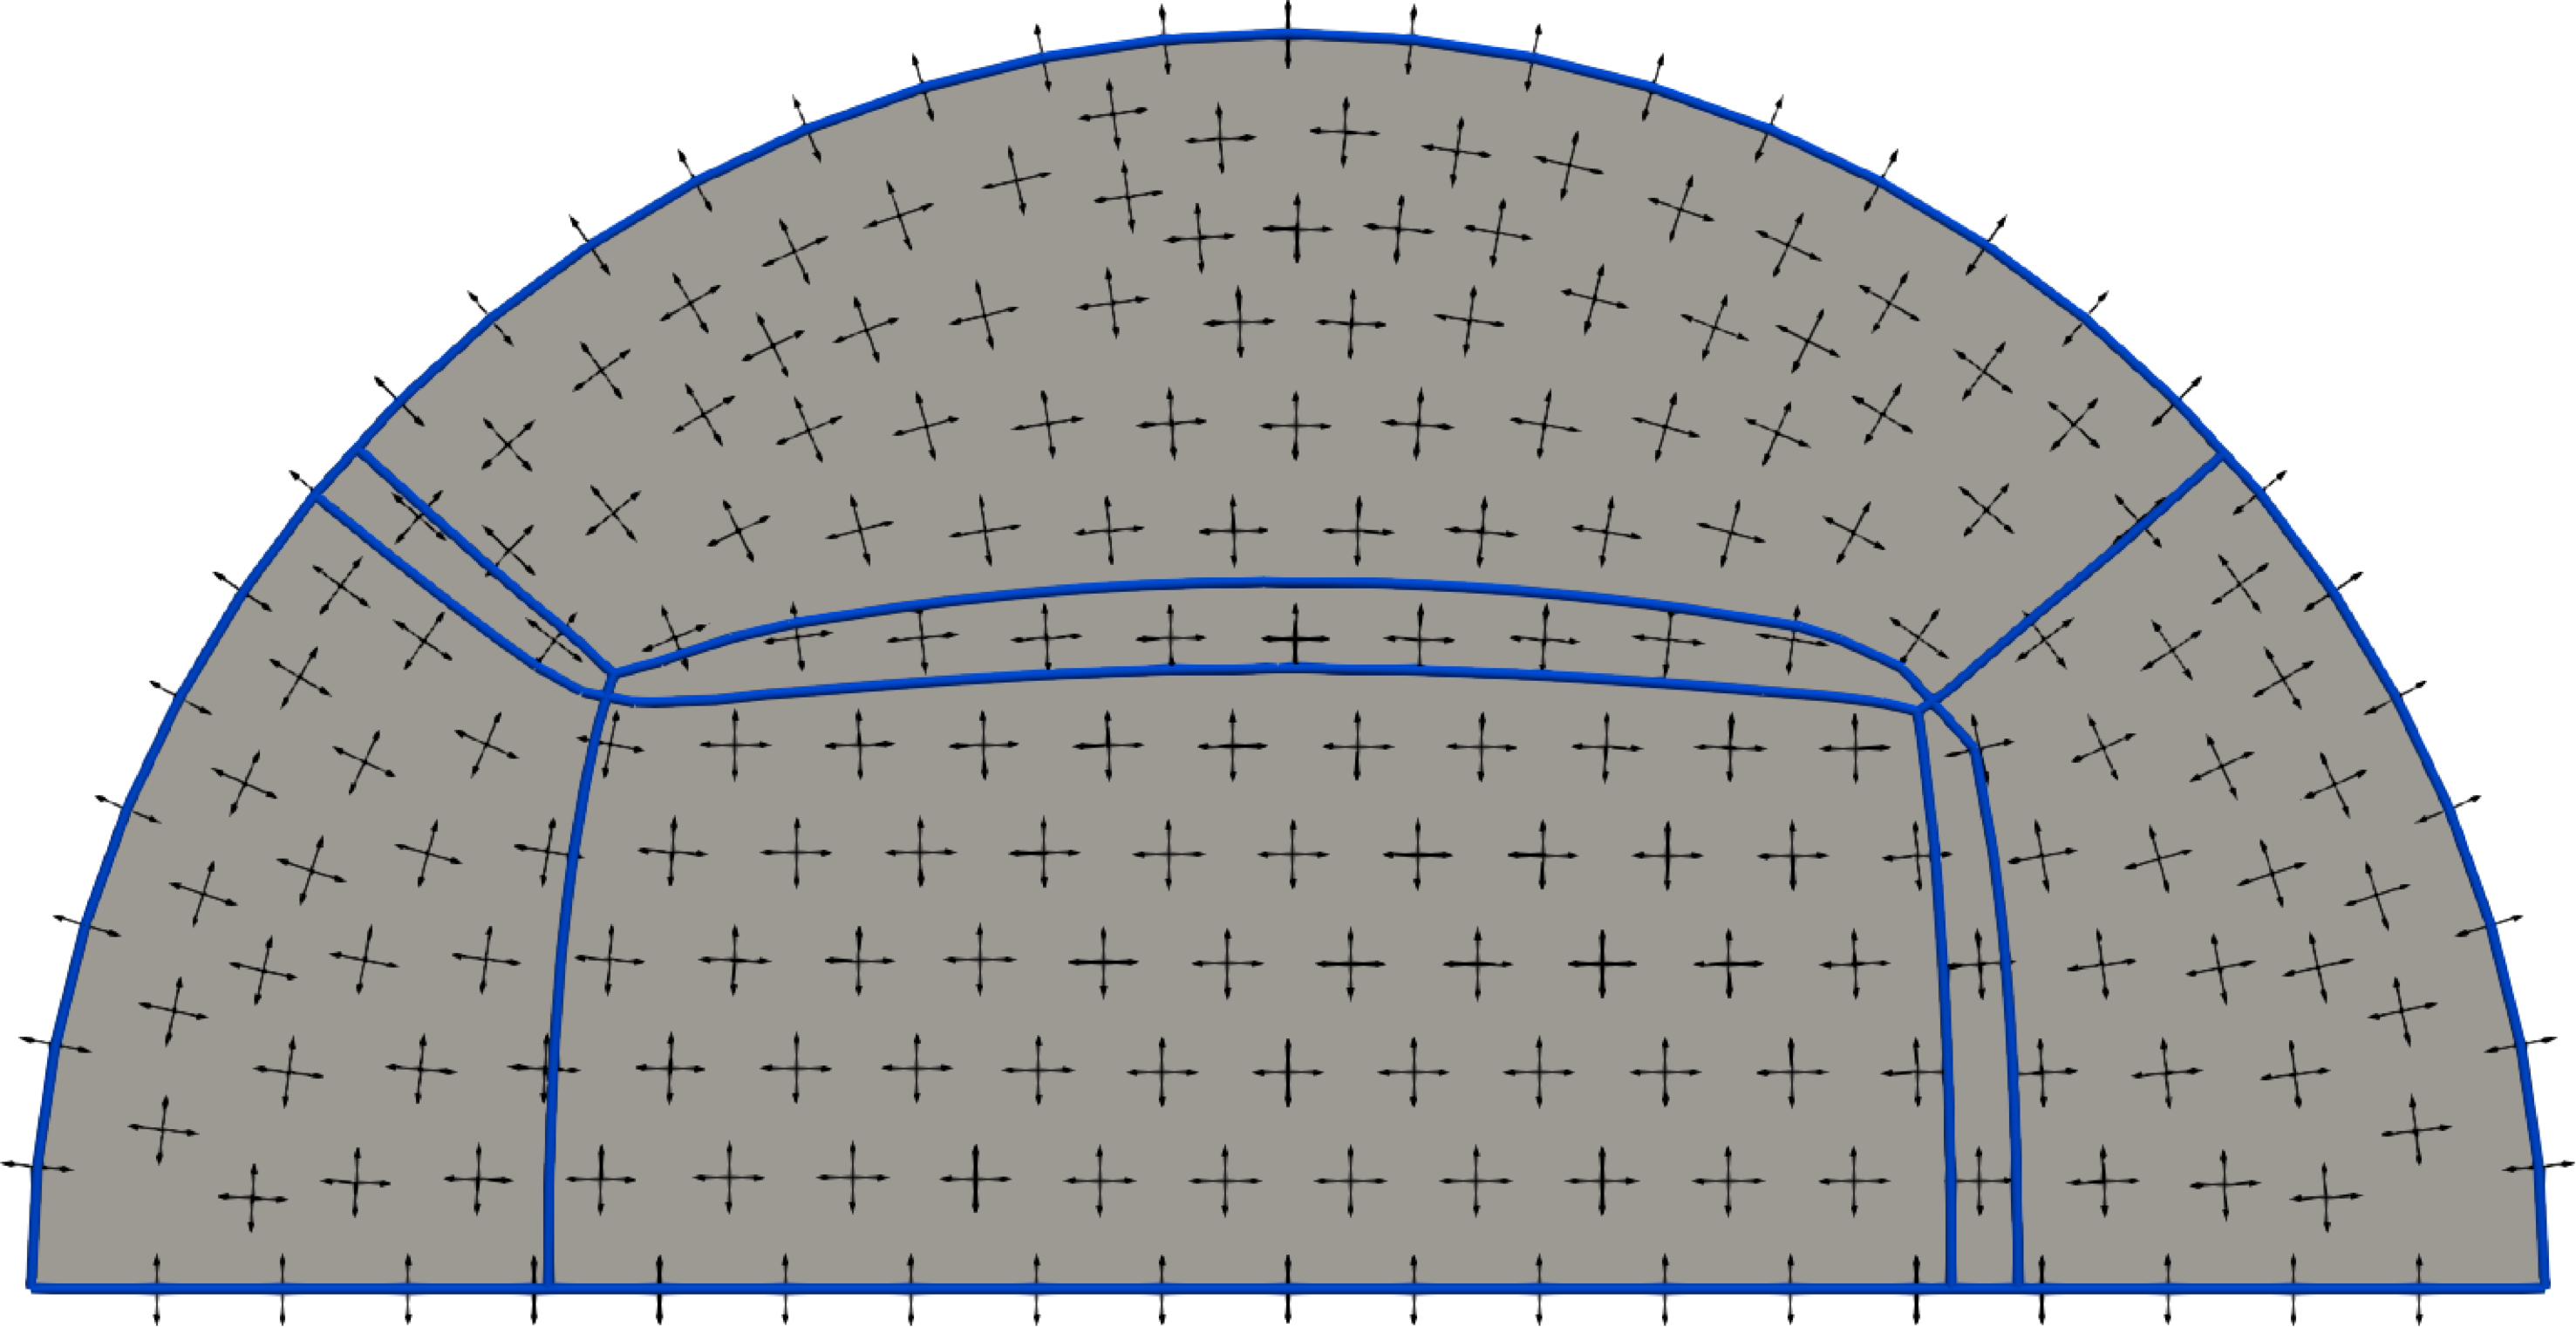
\includegraphics[width=\textwidth]{images/decoup_sans_fusion.pdf}
    \caption{Intégration de séparatrices sans fusion.}
    \label{fig:decoup_sans_fusion}
\end{subfigure}
\\[0.5cm]
\begin{subfigure}{0.65\textwidth}
    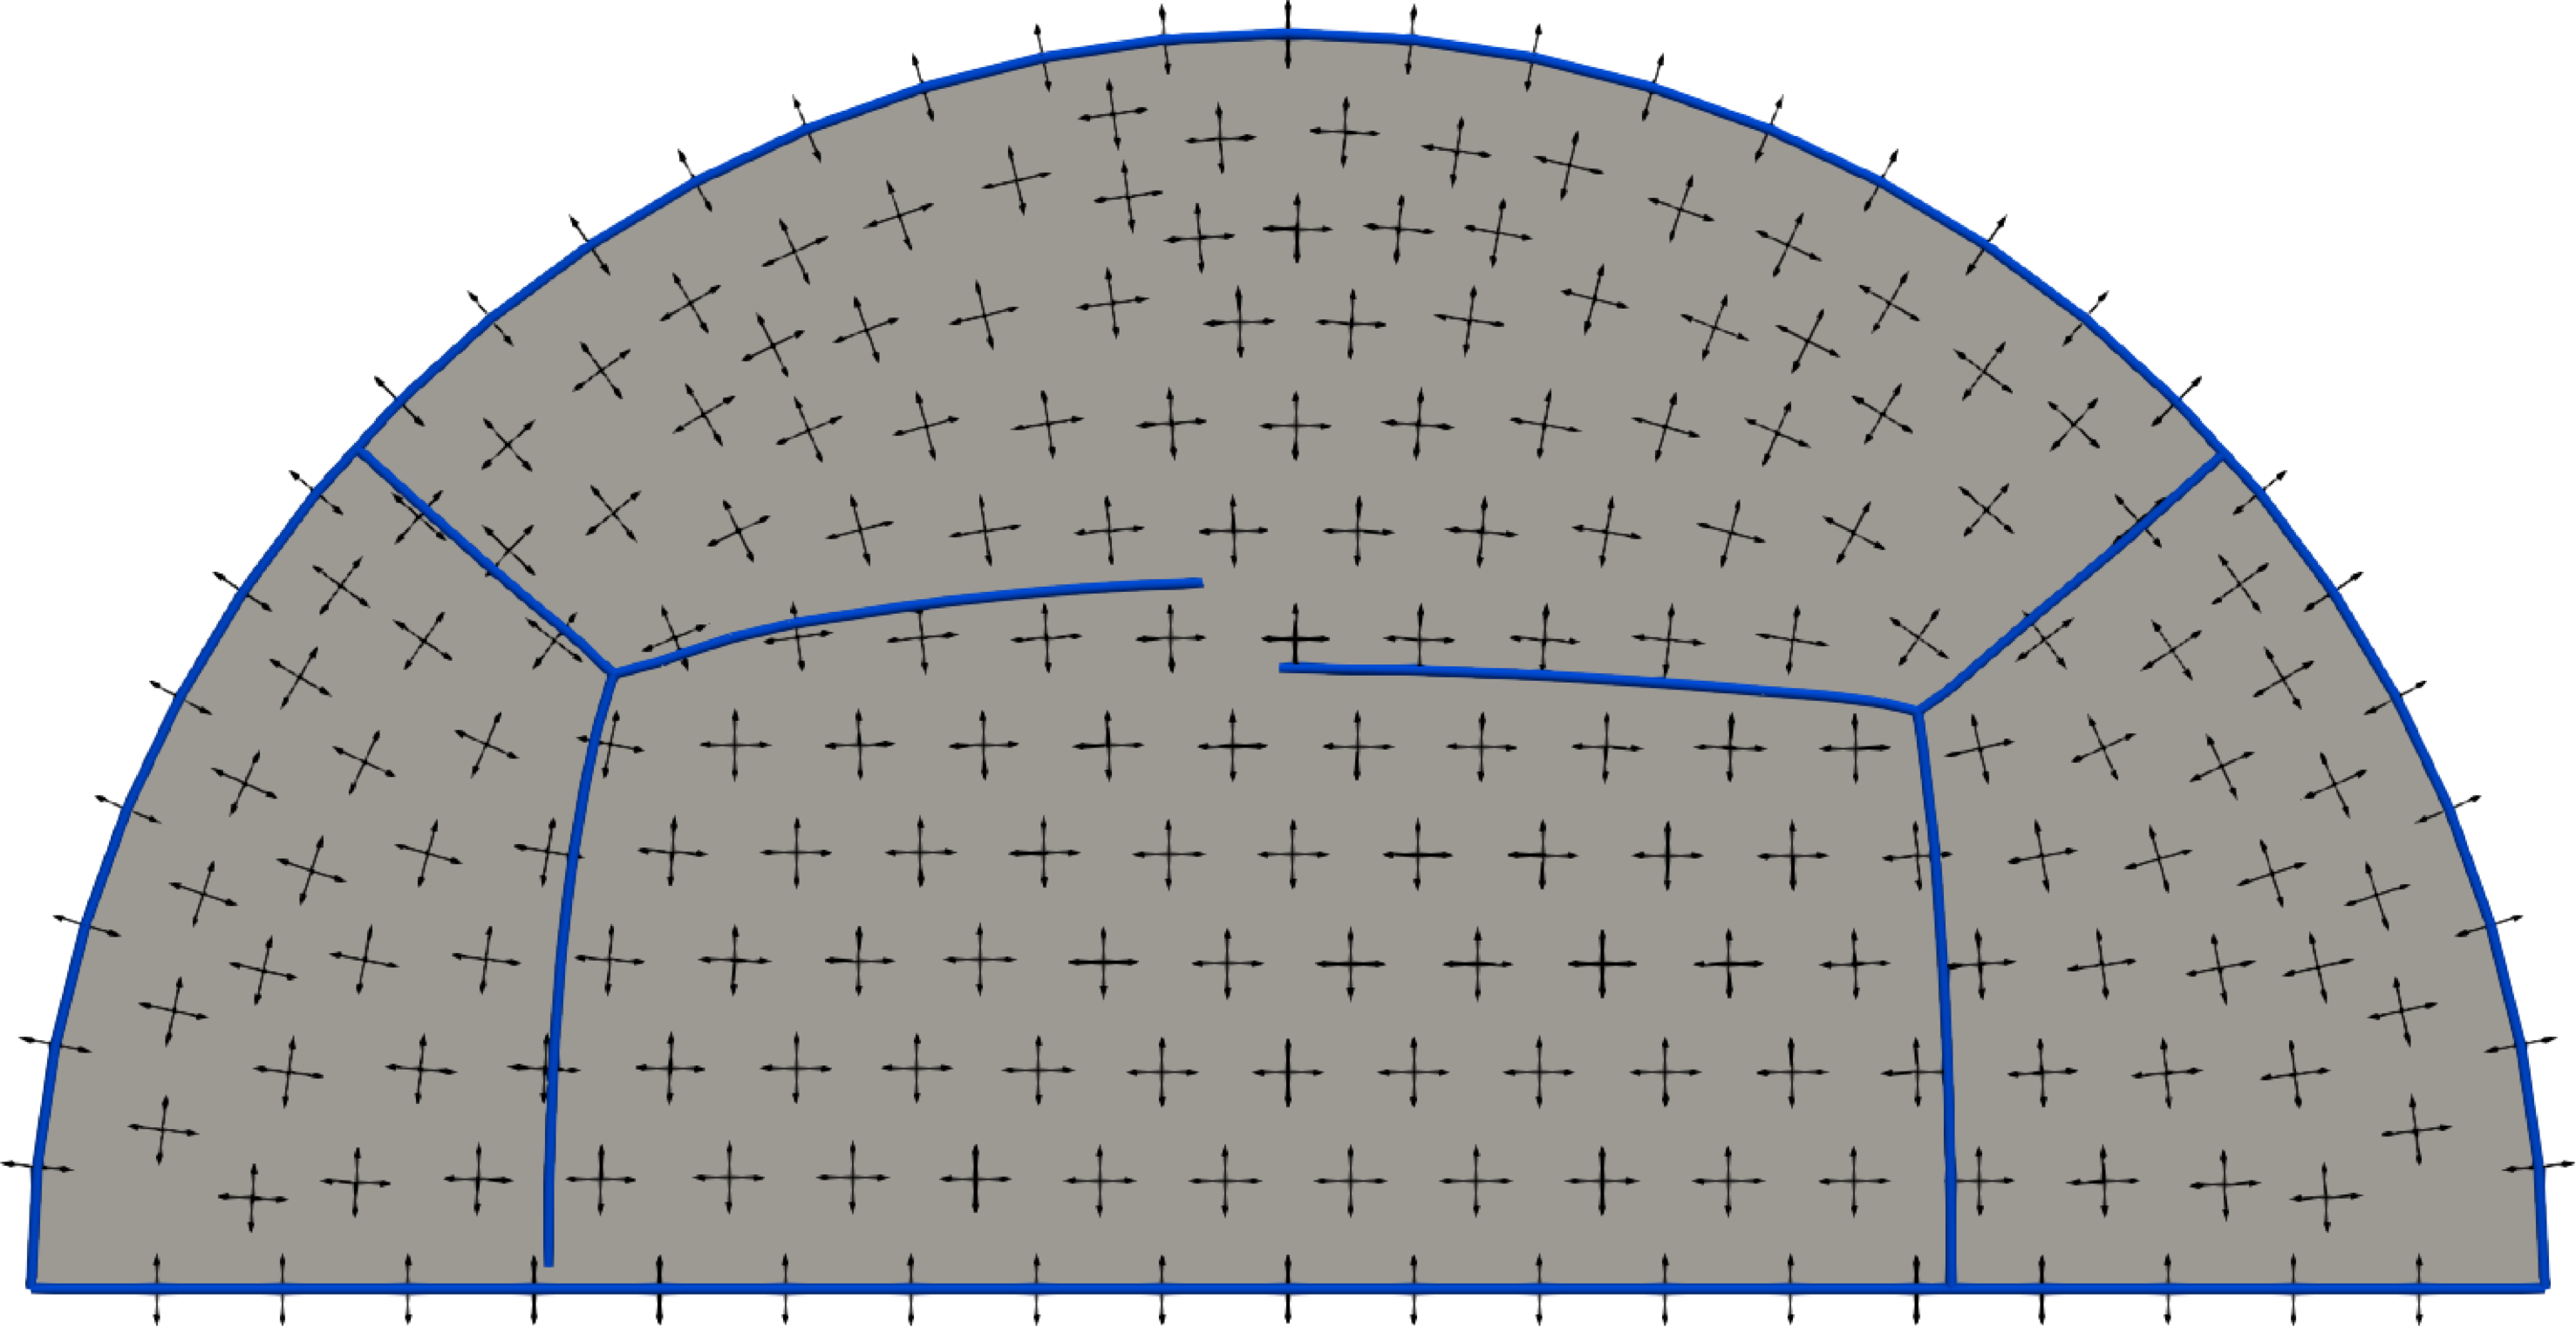
\includegraphics[width=\textwidth]{images/decoup_detect_fusion.pdf}
    \caption{Détection d'une fusion.}
    \label{fig:decoup_detect_fusion}
\end{subfigure}
\\[0.5cm]
\begin{subfigure}{0.65\textwidth}
    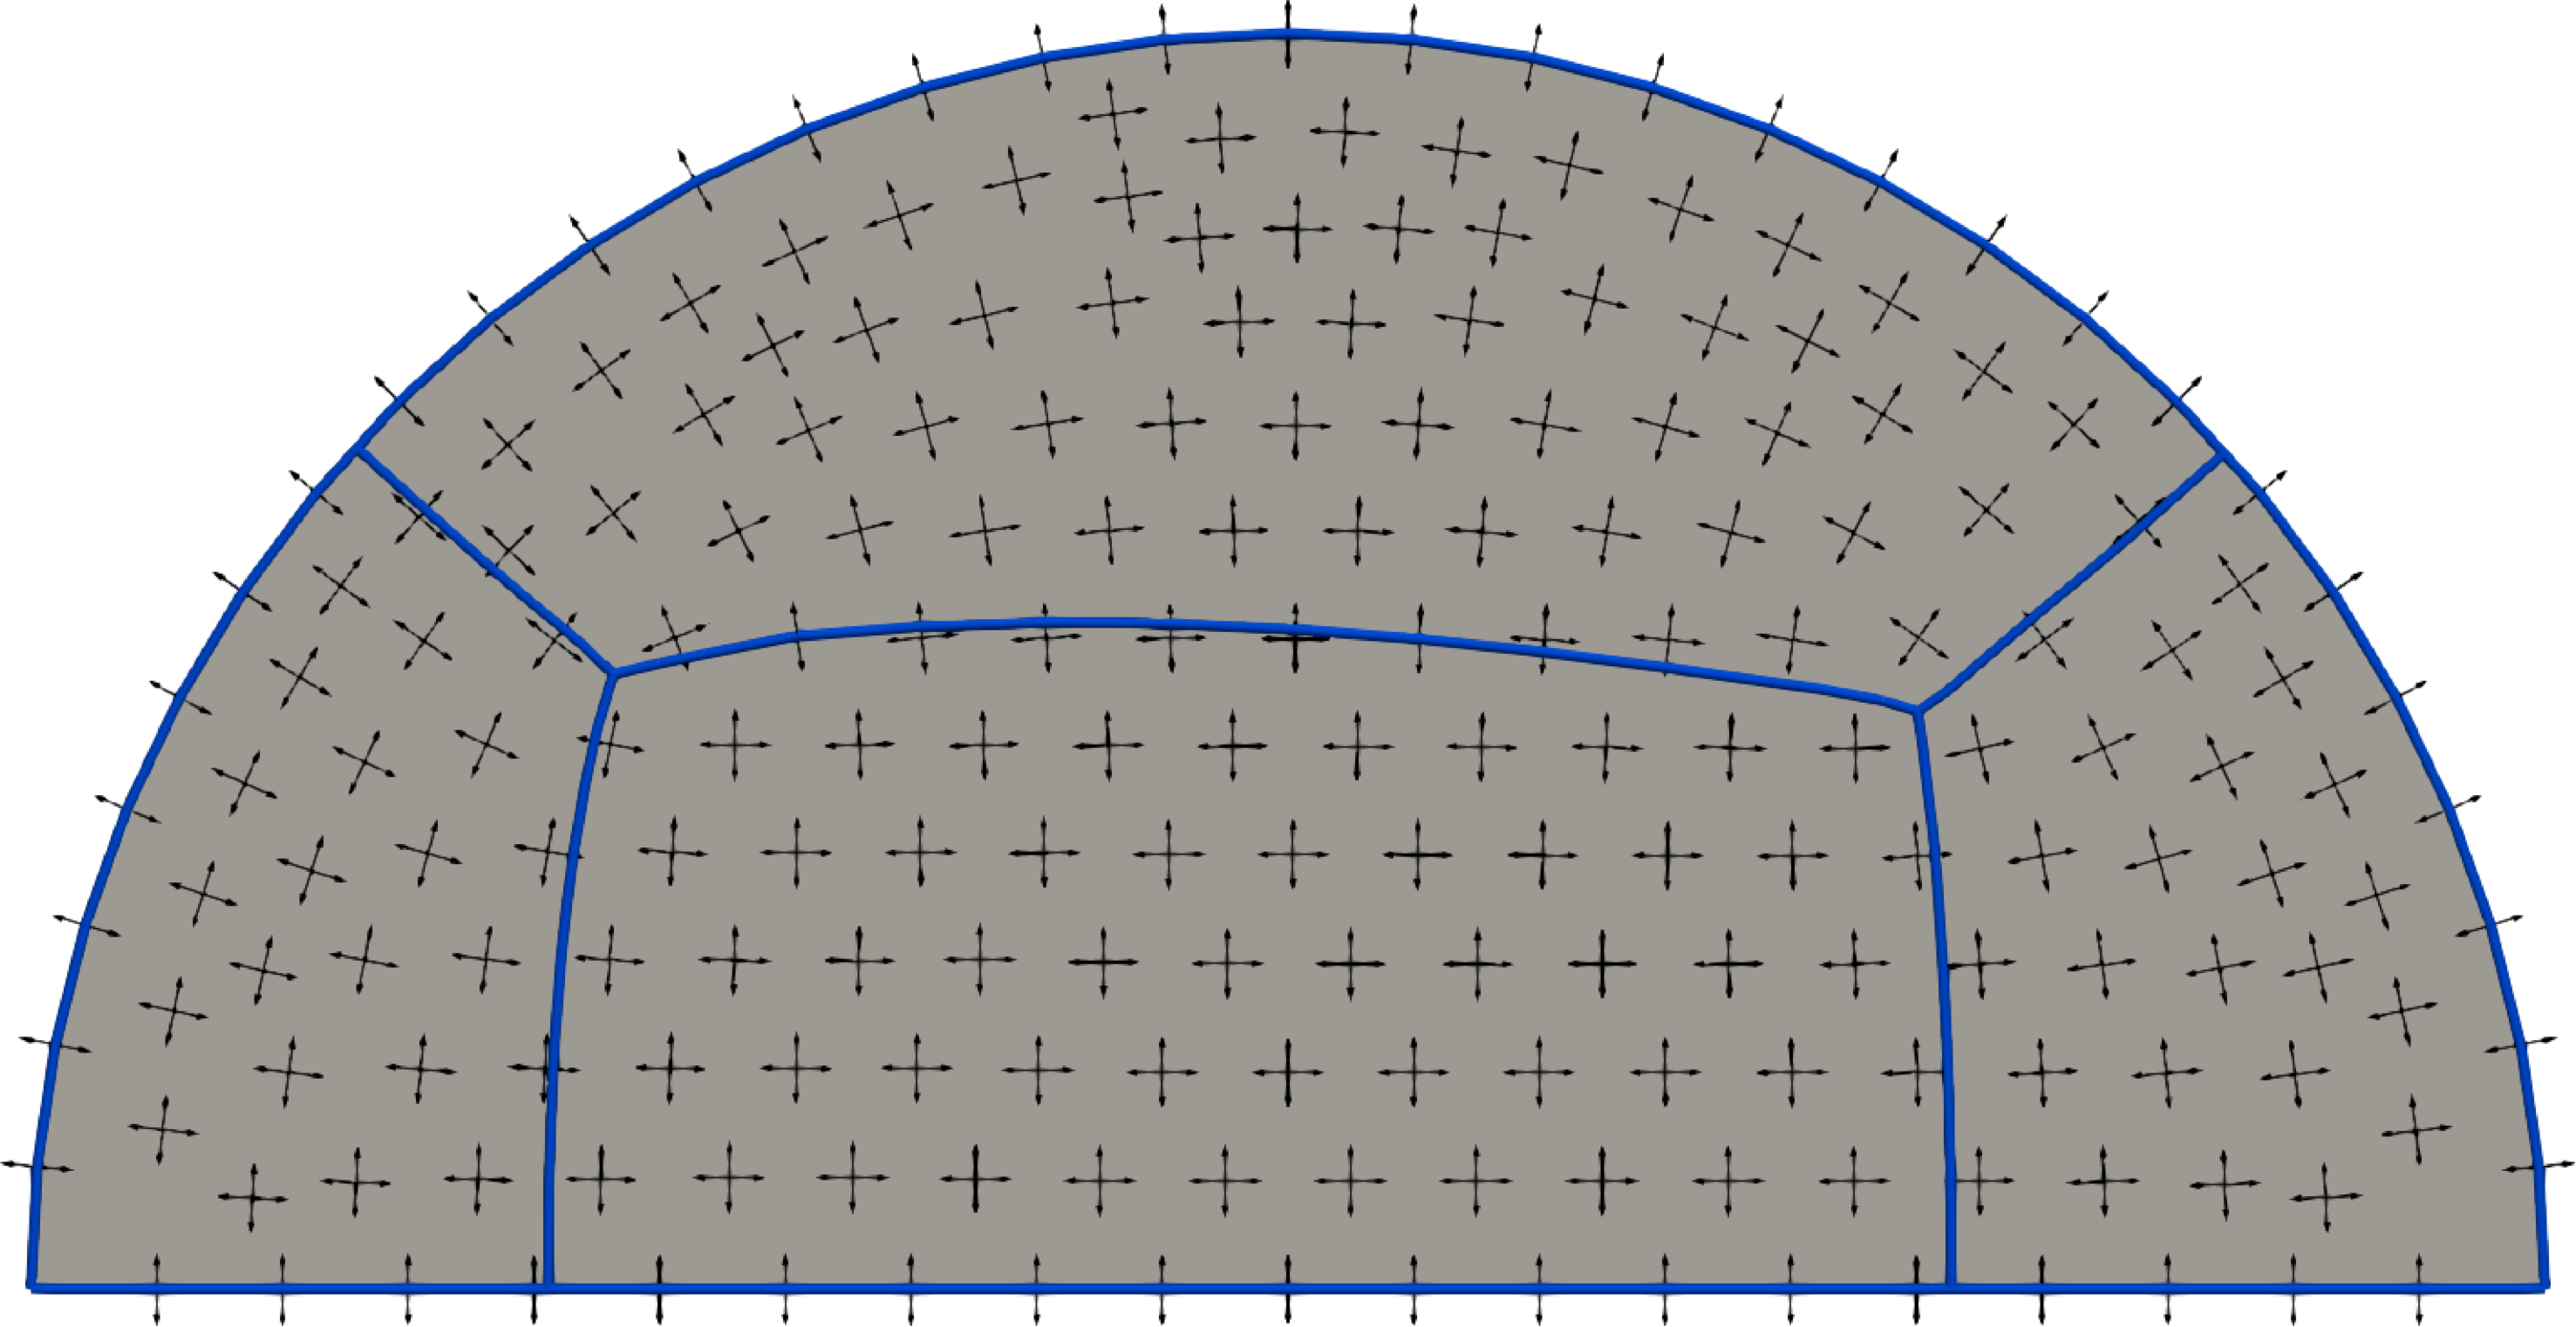
\includegraphics[width=\textwidth]{images/decoup_fusion.pdf}
    \caption{Intégration de séparatrices avec fusion.}
    \label{fig:decoup_fusion}
\end{subfigure}
\caption{Illustration de la fusion de séparatrices.}
\label{fig:fusion}
\end{figure}


lors de l'intégration d'une séparatrice, il peut arriver qu'elle doive traverser un triangle singulier. Dans ce cas, le processus d'intégration tel que décrit précédemment peut échouer (voir la figure \ref{fig:draw_streams_sing_1}). Cela résulte du fait que le champ d'angle associé au champ de croix dans le triangle n'est pas linéaire et présente des variations importantes. Pour surmonter ce problème, nous cherchons à représenter la séparatrice dans le triangle singulier en utilisant une succession d'autres segments calculés par un raffinement local du maillage à l'intérieur du triangle singulier. L'objectif est d'isoler le point singulier par rapport à la trajectoire de la séparatrice. Voici le procédé:

Considérons $T$ comme un triangle contenant un point singulier que doit traverser une séparatrice dont l'origine ne se trouve pas dans $T$. En d'autres termes, le dernier point calculé lors de la construction de cette séparatrice appartient à $T$ et le processus habituel d'intégration a généreé un segment traversant $T$ (voir figure \ref{fig:draw_streams_1}). Dans la suite nous appellerons ce "dernier point" le point d'entrée de la séparatrice dans $T$. On commence en subdivisant $T$ en quatre triangles. Cette subdivision peut être réalisée en reliant, par exemple, les milieux des arêtes de $T$ Il est essentiel de noter que si le point d'entrée coincide avec le milieu d'une arête, un autre point de cette arête doit être choisi pour la subdivision. L'objectif est que le point d'entrée se retrouve associé à un triangle issu de la subdivision et ne contenant pas de point singulier. On peut alors appliquer le processus d'intégration dans ce triangle, tel que décrit précédemment (voir figure \ref{fig:draw_streams_sing_2}). Il ne reste plus qu'à itérer ce schéma de construction jusqu'à ce que la séparatrice sorte de la partie du plan correspondant au triangle initial (voir figures \ref{fig:draw_streams_sing_3} et \ref{fig:draw_streams_sing_4}). On se retouve ainsi avec un raffinement local et adapté du maillage en fonction de la trajectoire de la séparatrice ce qui permet en pratique de ne pas raffiner l'intégralité du maillage pour avoir une bonne approximation de la séparatice. Il convient de souligner qu'il n'est pas nécessaire d'apporter des modifications locales au maillage dans sa globalité. Après avoir construit la séparatrice, nous conservons uniquement ses points de passage et supprimons tout raffinement local utilisé.


\paragraph{Fusion de séparatrices:} 


de manière similaire à ce qui est réalisé dans \cite{marcon2019high}, les séparatrices du champ de croix sont construites simultanément en incrémentant chacune d'elles progressivement, et la rencontre entre deux séparatrices est anticipée en comparant à chaque incrément, d'une part, la distance entre les derniers points calculés et, d'autre part, les directions des derniers segments construits. En d'autres termes, on cherche à déterminer si, à un moment donné, deux séparatrices données avancent dans des directions opposées et si elles sont suffisamment proches l'une de l'autre. On compare ces deux mesures à des seuils prédéfinis, et en fonction du résultat, on décide de fusionner ou non les deux séparatrices.

La fusion se réalise en créant une nouvelle séparatrice par une fusion linéaire des points des deux séparatrices impliquées. Pour se faire, chaque séparatrice est prolongée à travers $\Omega_h$ jusqu'à atteindre la position de départ de l'autre, tout en maintenant le même nombre de points pour chacune des séparatrices. L'intérêt de fusionner les séparatrices réside dans la réduction de leur nombre, ce qui se traduit directement par une diminution du nombre de régions générées lors du découpage du domaine. Nous illustrons la fusion de deux séparatrices sur la figure \ref{fig:fusion}. Il est remarquable que la non-fusion des séparatrices génère davantage de régions, certaines étant fortement étirées et non homogènes par rapport aux autres, ce qui est une source potentielle d'inhomogénéité des mailles dans les maillages quadrilatéraux.


\begin{figure}[h!]
\centering
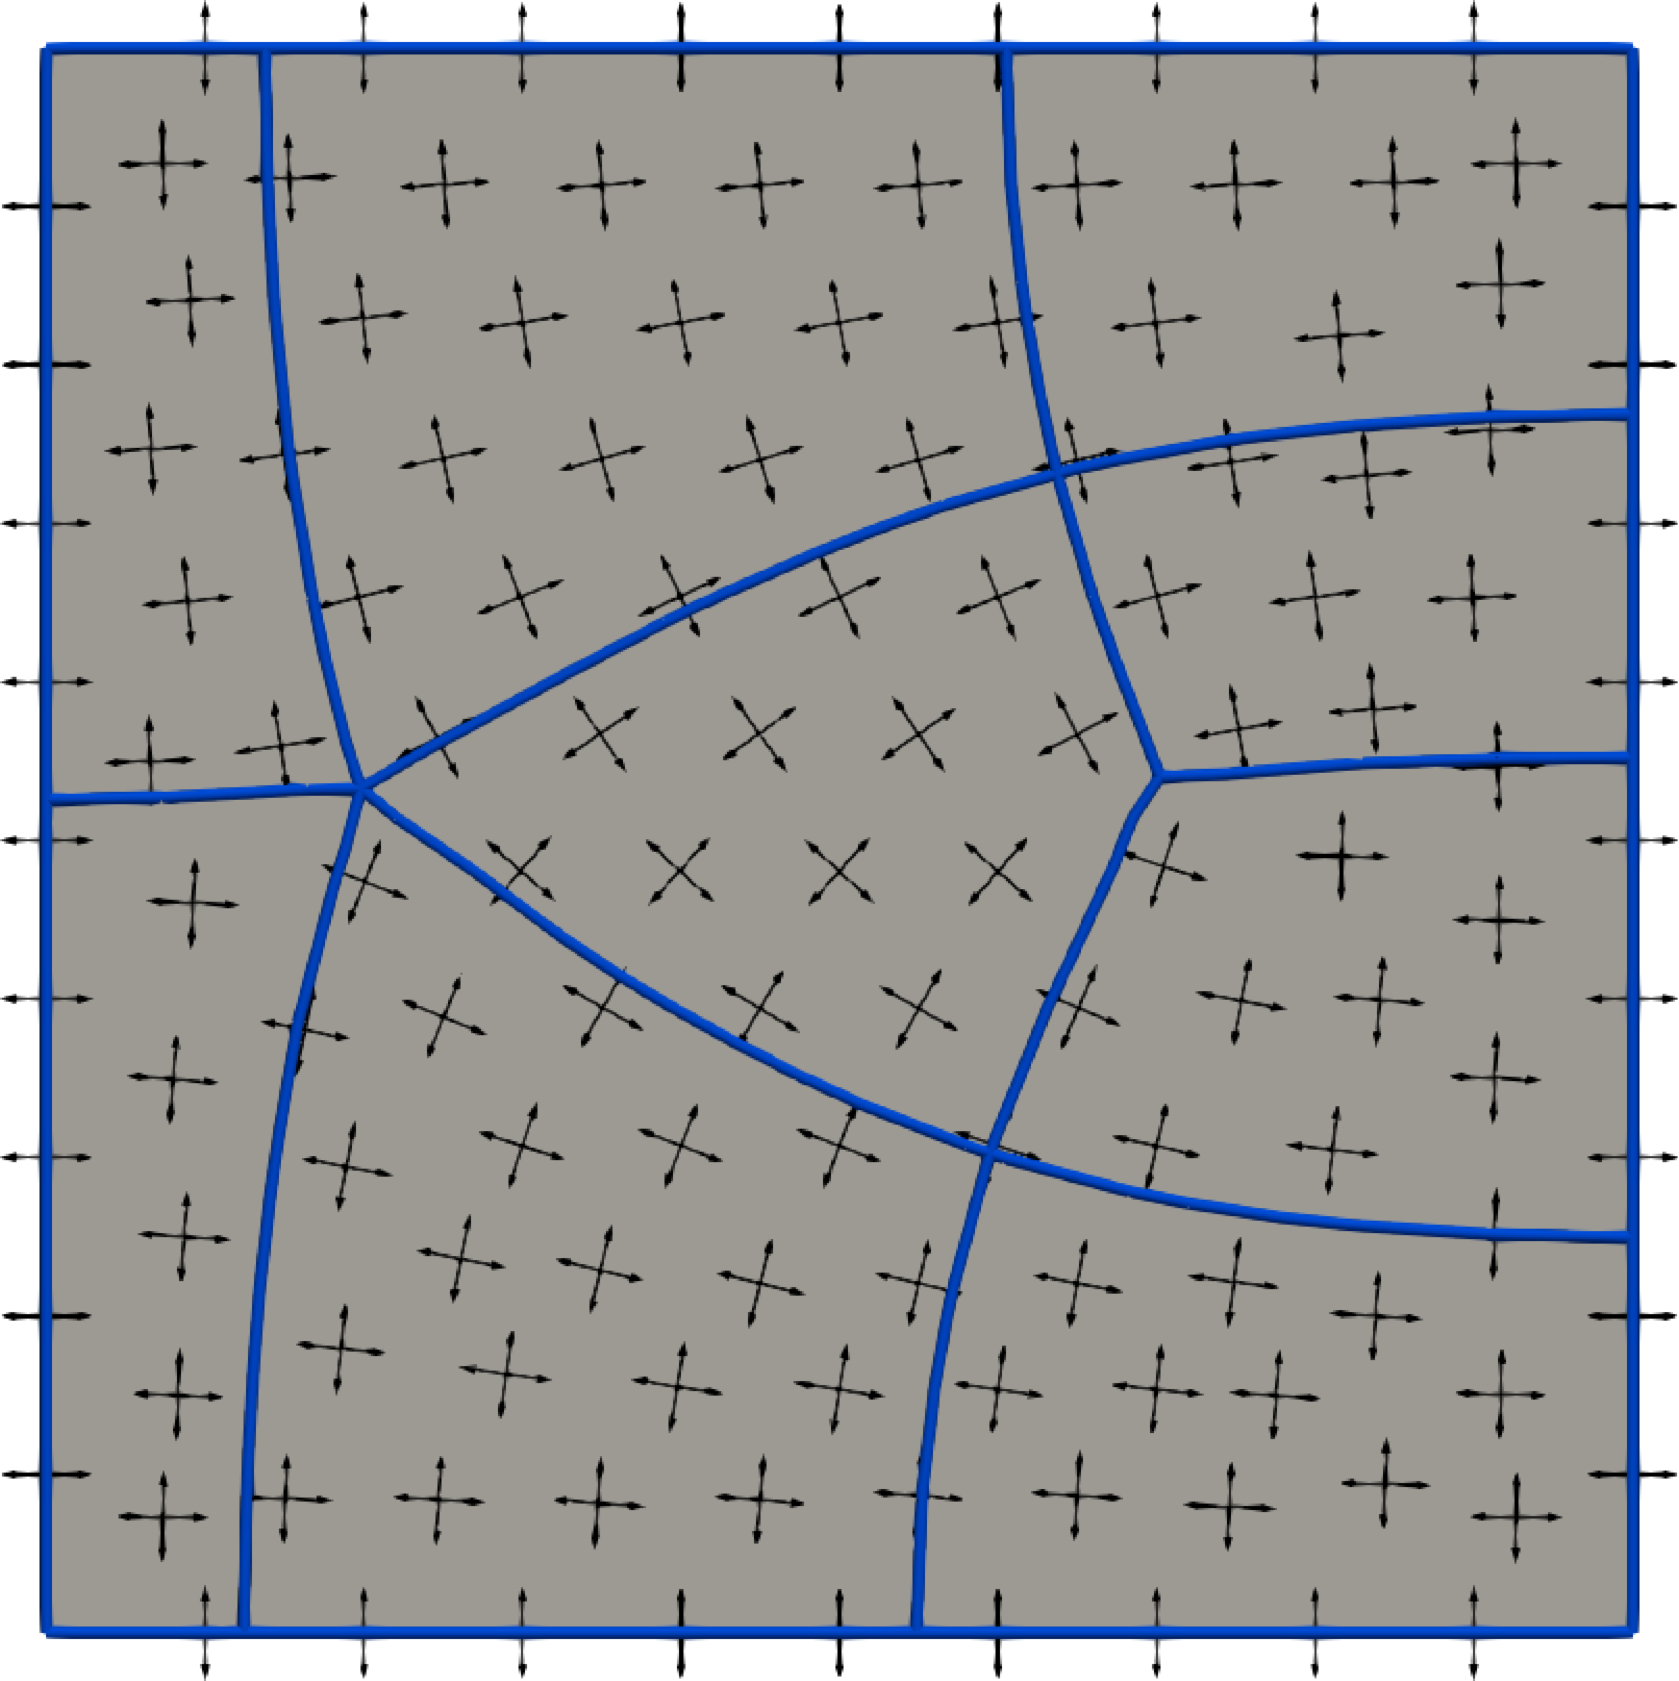
\includegraphics[scale=0.2755]{images/eclatement_1.pdf}
\hfill
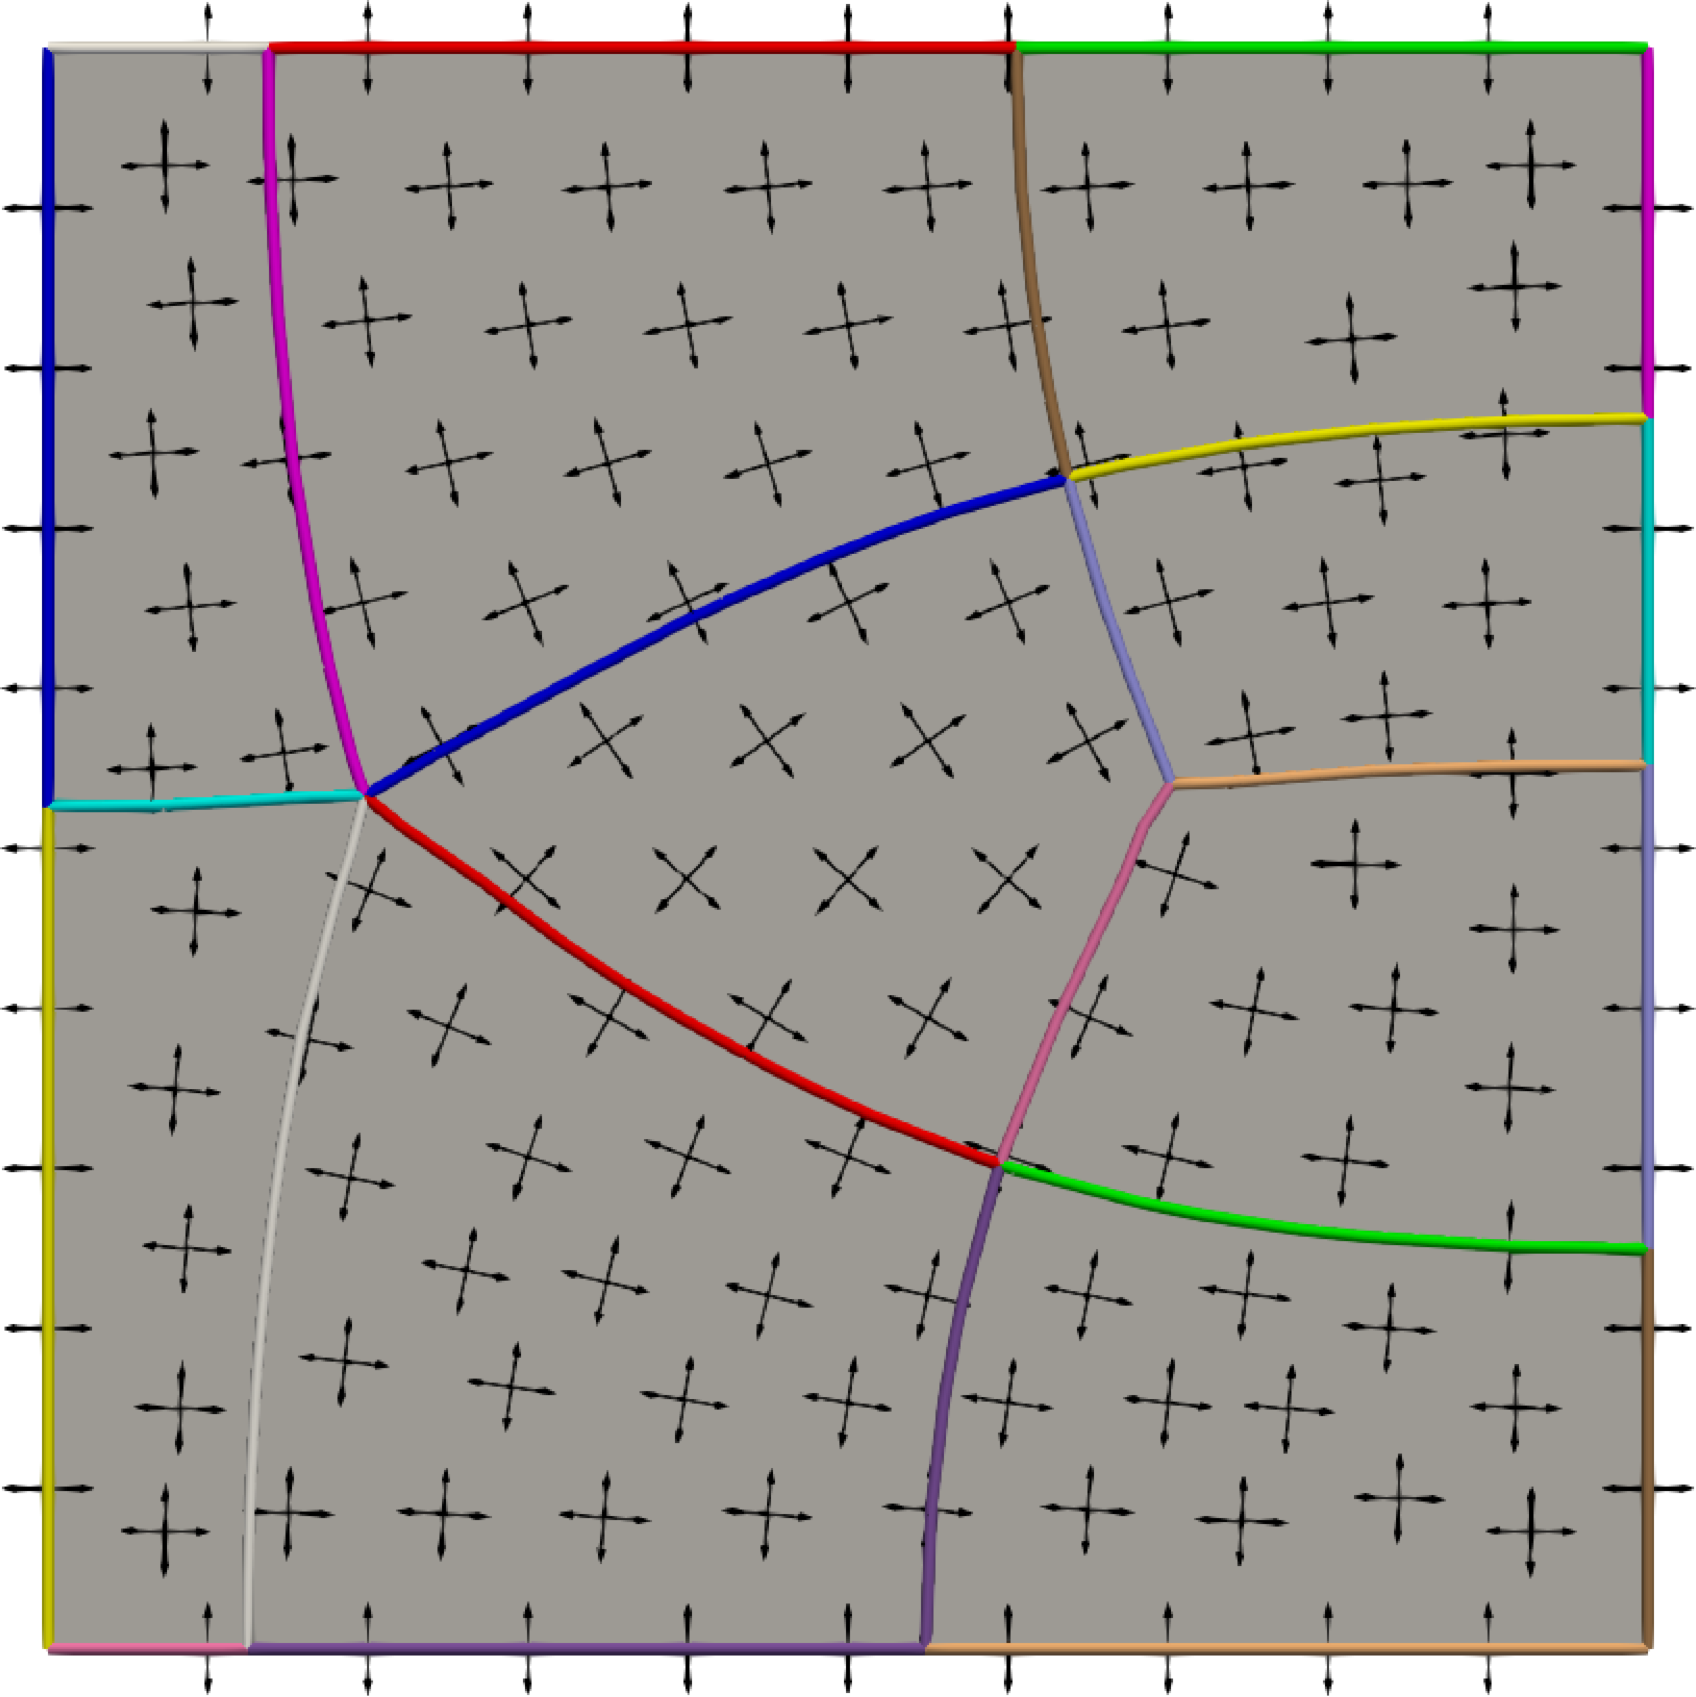
\includegraphics[scale=0.2755]{images/intersect_stream.pdf}
\caption{Direction de sortie différentes.}
\label{fig:detect_intersection}
\end{figure}


\subsection{Assemblage des partitions}

Une fois les séparatrices construites, nous procédons à la subdivision du maillage triangulaire $\Omega_h$ en plusieurs régions distinctes. Cette opération consiste à modifier $\Omega_h$ en y intégrant les segments formant les séparatrices, créant ainsi un nouveau maillage. Notre objectif est de délimiter chaque région sous forme de sous-maillage distinct de $\Omega_h$. Ce processus débute par l'identification des frontières de ces régions via la localisation des points d'intersection entre les séparatrices, suivie de l'extraction de chaque région individuelle.

\paragraph{Intersections de séparatrices:}

Comme annoncé, la première étape de ce processus consiste à déterminer les frontières des régions. La recherche des points d'intersection entre les séparatrices peut être réalisée localement dans chaque triangle et simultanément. Étant donné que les séparatrices sont constituées de segments, il suffit de vérifier l'intersection de ces segments les uns par rapport aux autres. En découpant les séparatrices au niveau de ces points d'intersection, cela met en évidence les contours des régions, comme illustré sur la figure \ref{fig:detect_intersection}.

\paragraph{Identification des partitions:}
Dans cette phase, notre objectif est de découper le maillage triangulaire initial $\Omega_h$ en plusieurs sous-maillages, représentant chacun une partition. Pour y parvenir, nous enrichissons $\Omega_h$ en y insérant les points qui constituent les séparatrices, puis nous ajustons le maillage pour qu'il intègre les segments formés par ces séparatrices. Cette étape de modification du maillage peut être réalisée localement au niveau de chaque triangle de $\Omega_h$, exploitant ainsi les capacités de calcul parallèle pour accélérer le processus.

Considérons $T$ comme un triangle de $\Omega_h$ traversé par certains segments des séparatrices construites (voir figure \ref{fig:exemple_insert_pt_0}). Pour insérer ces segments dans $T$, nous commençons par introduire les points de bord de ces segments tout en conservant la structure en triangles du triangle initial. De cette manière, nous obtenons un raffinement triangulaire de $T$. Pour insérer un point $p$ dans $T$ (s'il ne fait pas encore parti du raffinement), on commence par identifier l'élément ou des deux éléments de $T$ contenant ce point. Ensuite, l'insertion de $p$ s'opère dans ces éléments en générant de nouveaux triangles de la manière suivante (voir figure \ref{fig:insert_pt}):\\
\begin{itemize}
 \item si $p$ se trouve à l'intérieur d'un triangle $K\subset T$ alors son insertion génère trois nouveaux triangles par liaison de $p$ aux sommets de $K$.\\
 \item si $p$ se trouve sur une arête d'un triangle $K\subset T$, alors don insertion engendre deux nouveaux triangles par liaison de $p$ au sommet opposé à l'arête concernée.
\end{itemize}

\begin{figure}[h!]
\centering
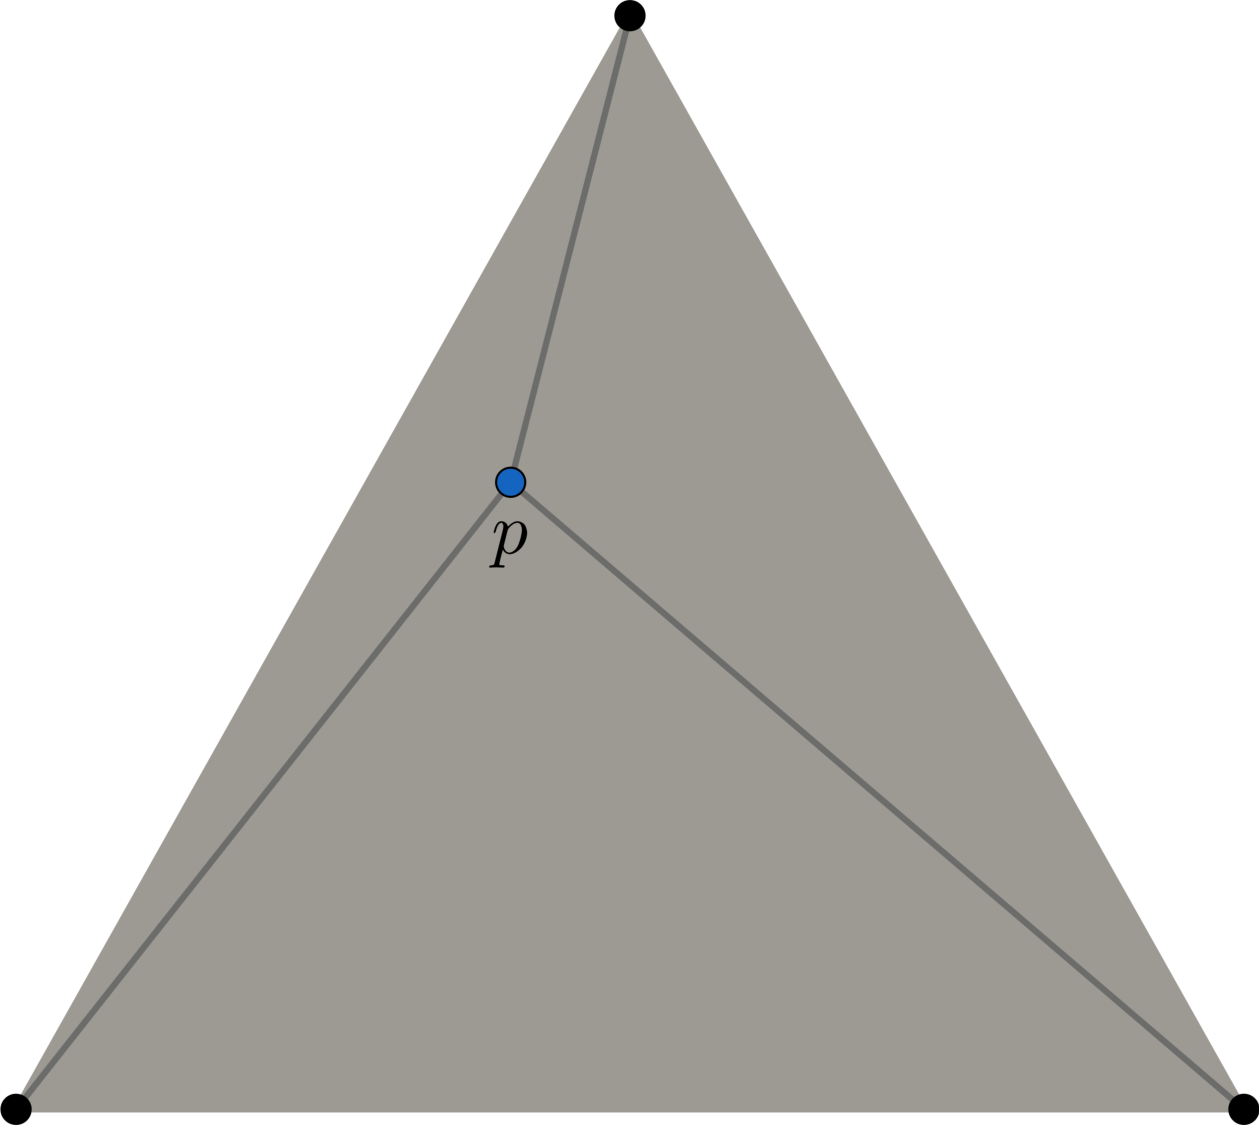
\includegraphics[scale=0.37]{images/insert_pt_1.pdf}\hfill
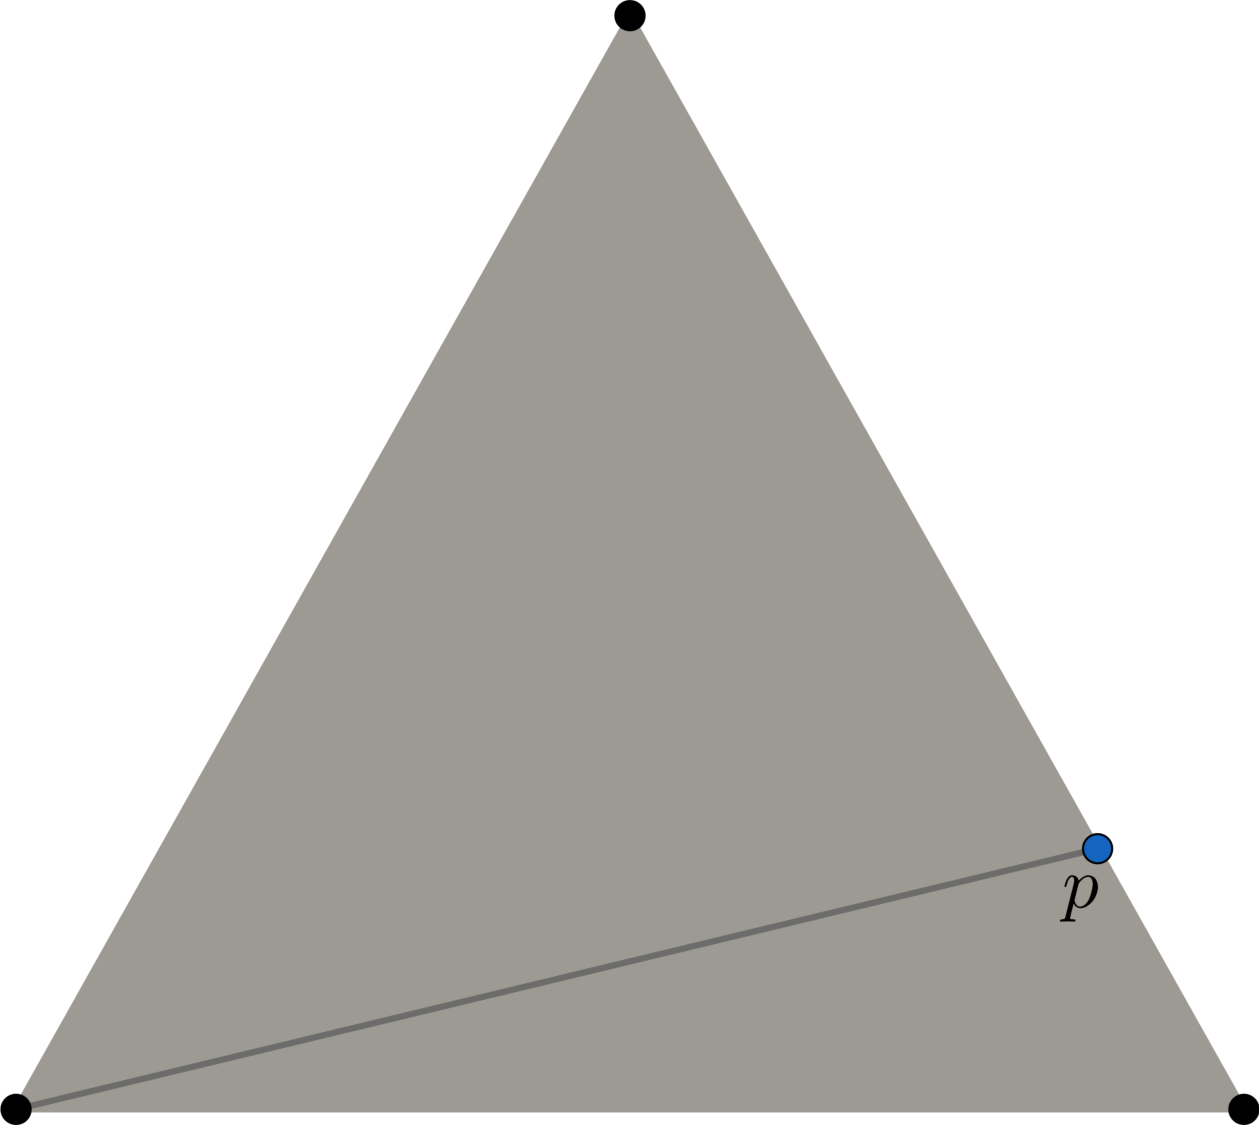
\includegraphics[scale=0.37]{images/insert_pt_2.pdf}
\caption{Direction de sortie différentes.}
\label{fig:insert_pt}
\end{figure}

\begin{figure}[h!]
\centering
\begin{subfigure}{0.45\textwidth}
    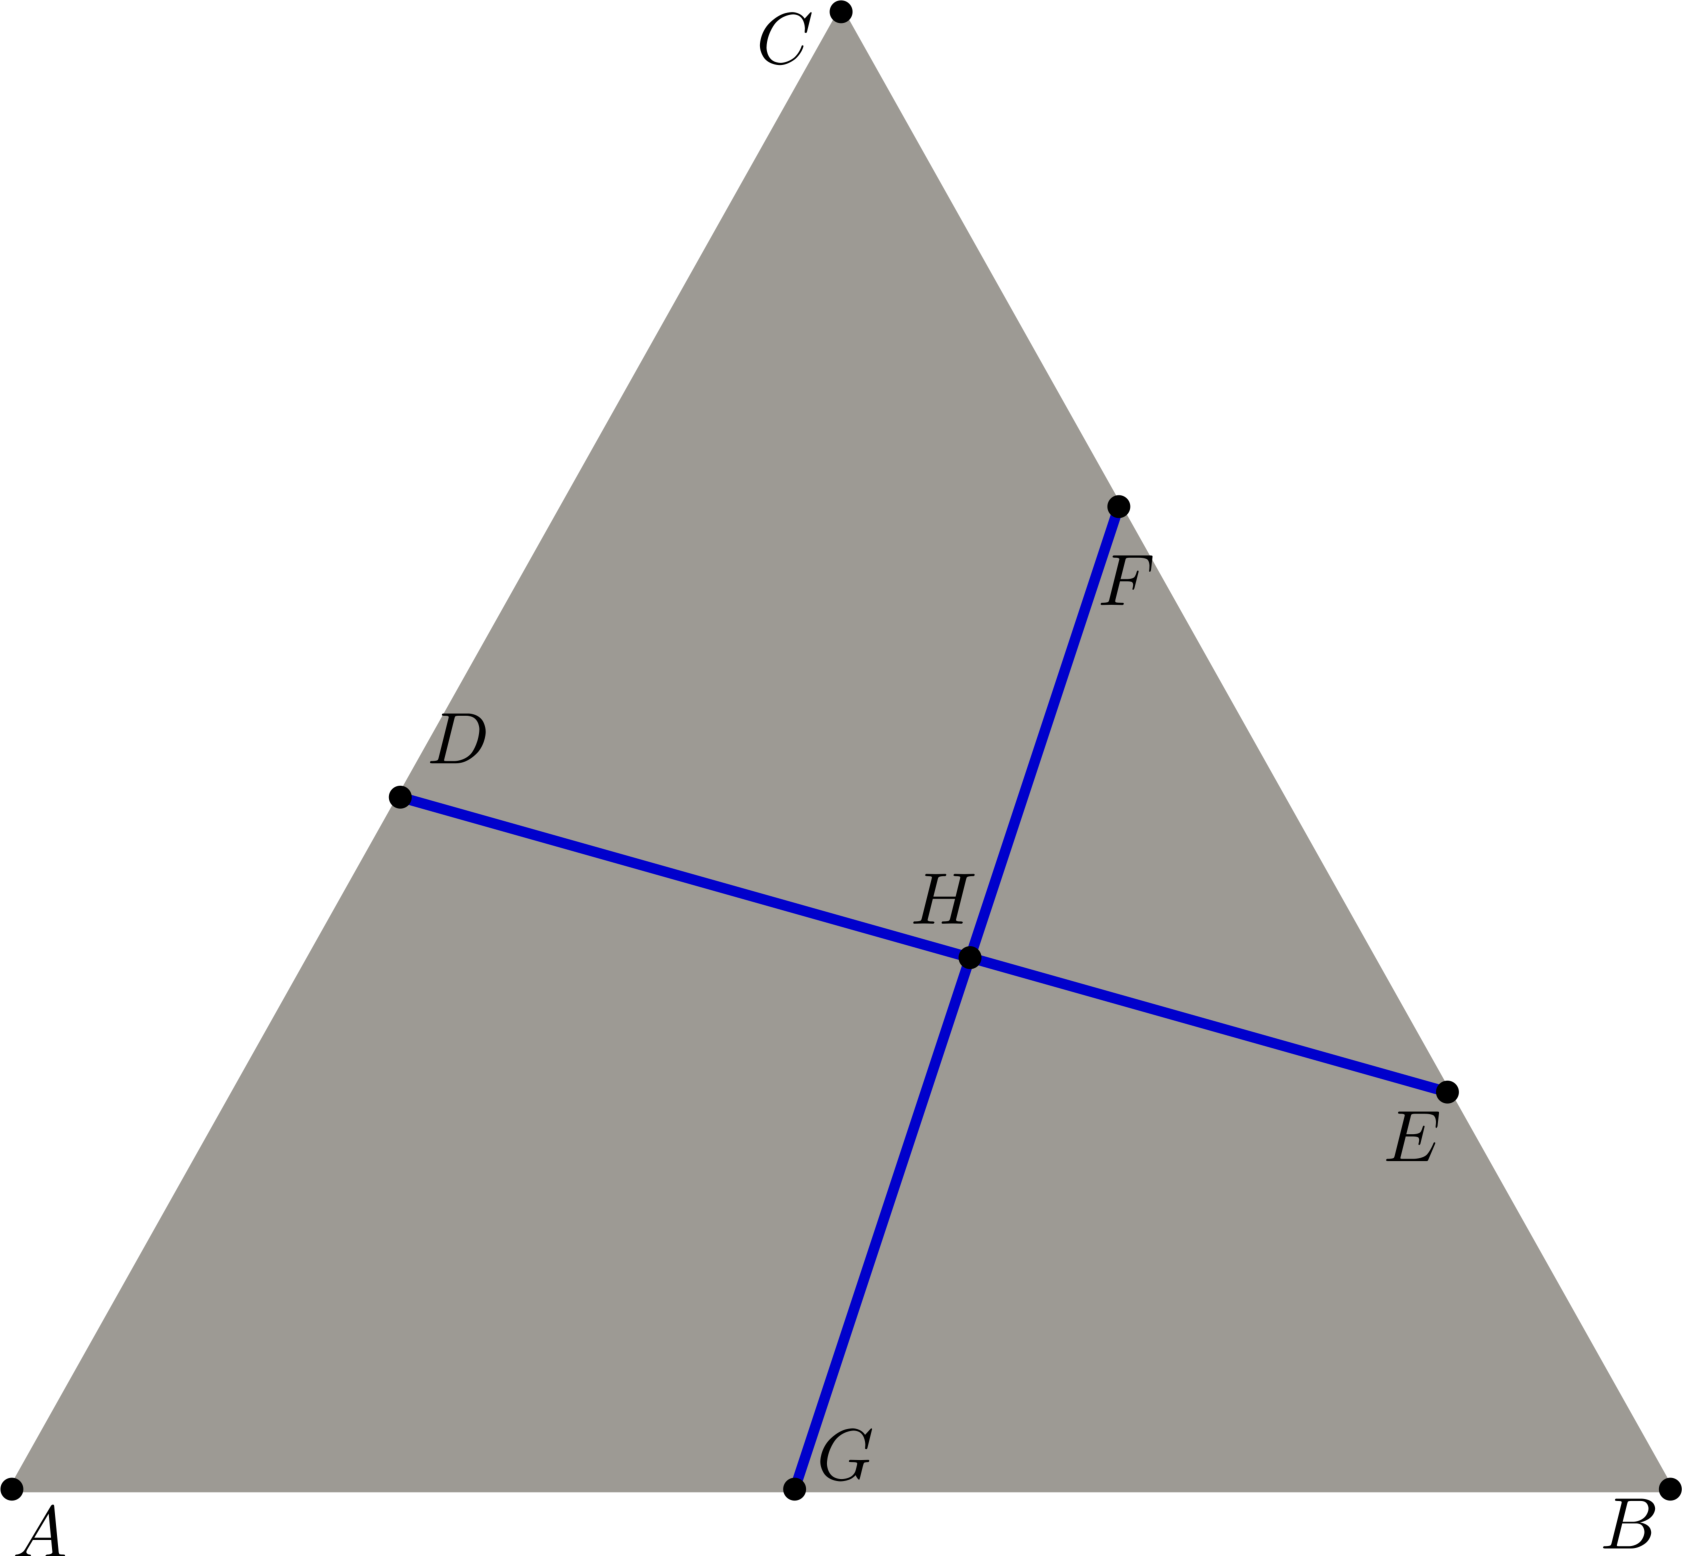
\includegraphics[width=\textwidth]{images/decoup_triangle.pdf}
    \caption{Triangle traversé par des séparatrices.}
    \label{fig:exemple_insert_pt_0}
\end{subfigure}
\hfill
\begin{subfigure}{0.45\textwidth}
    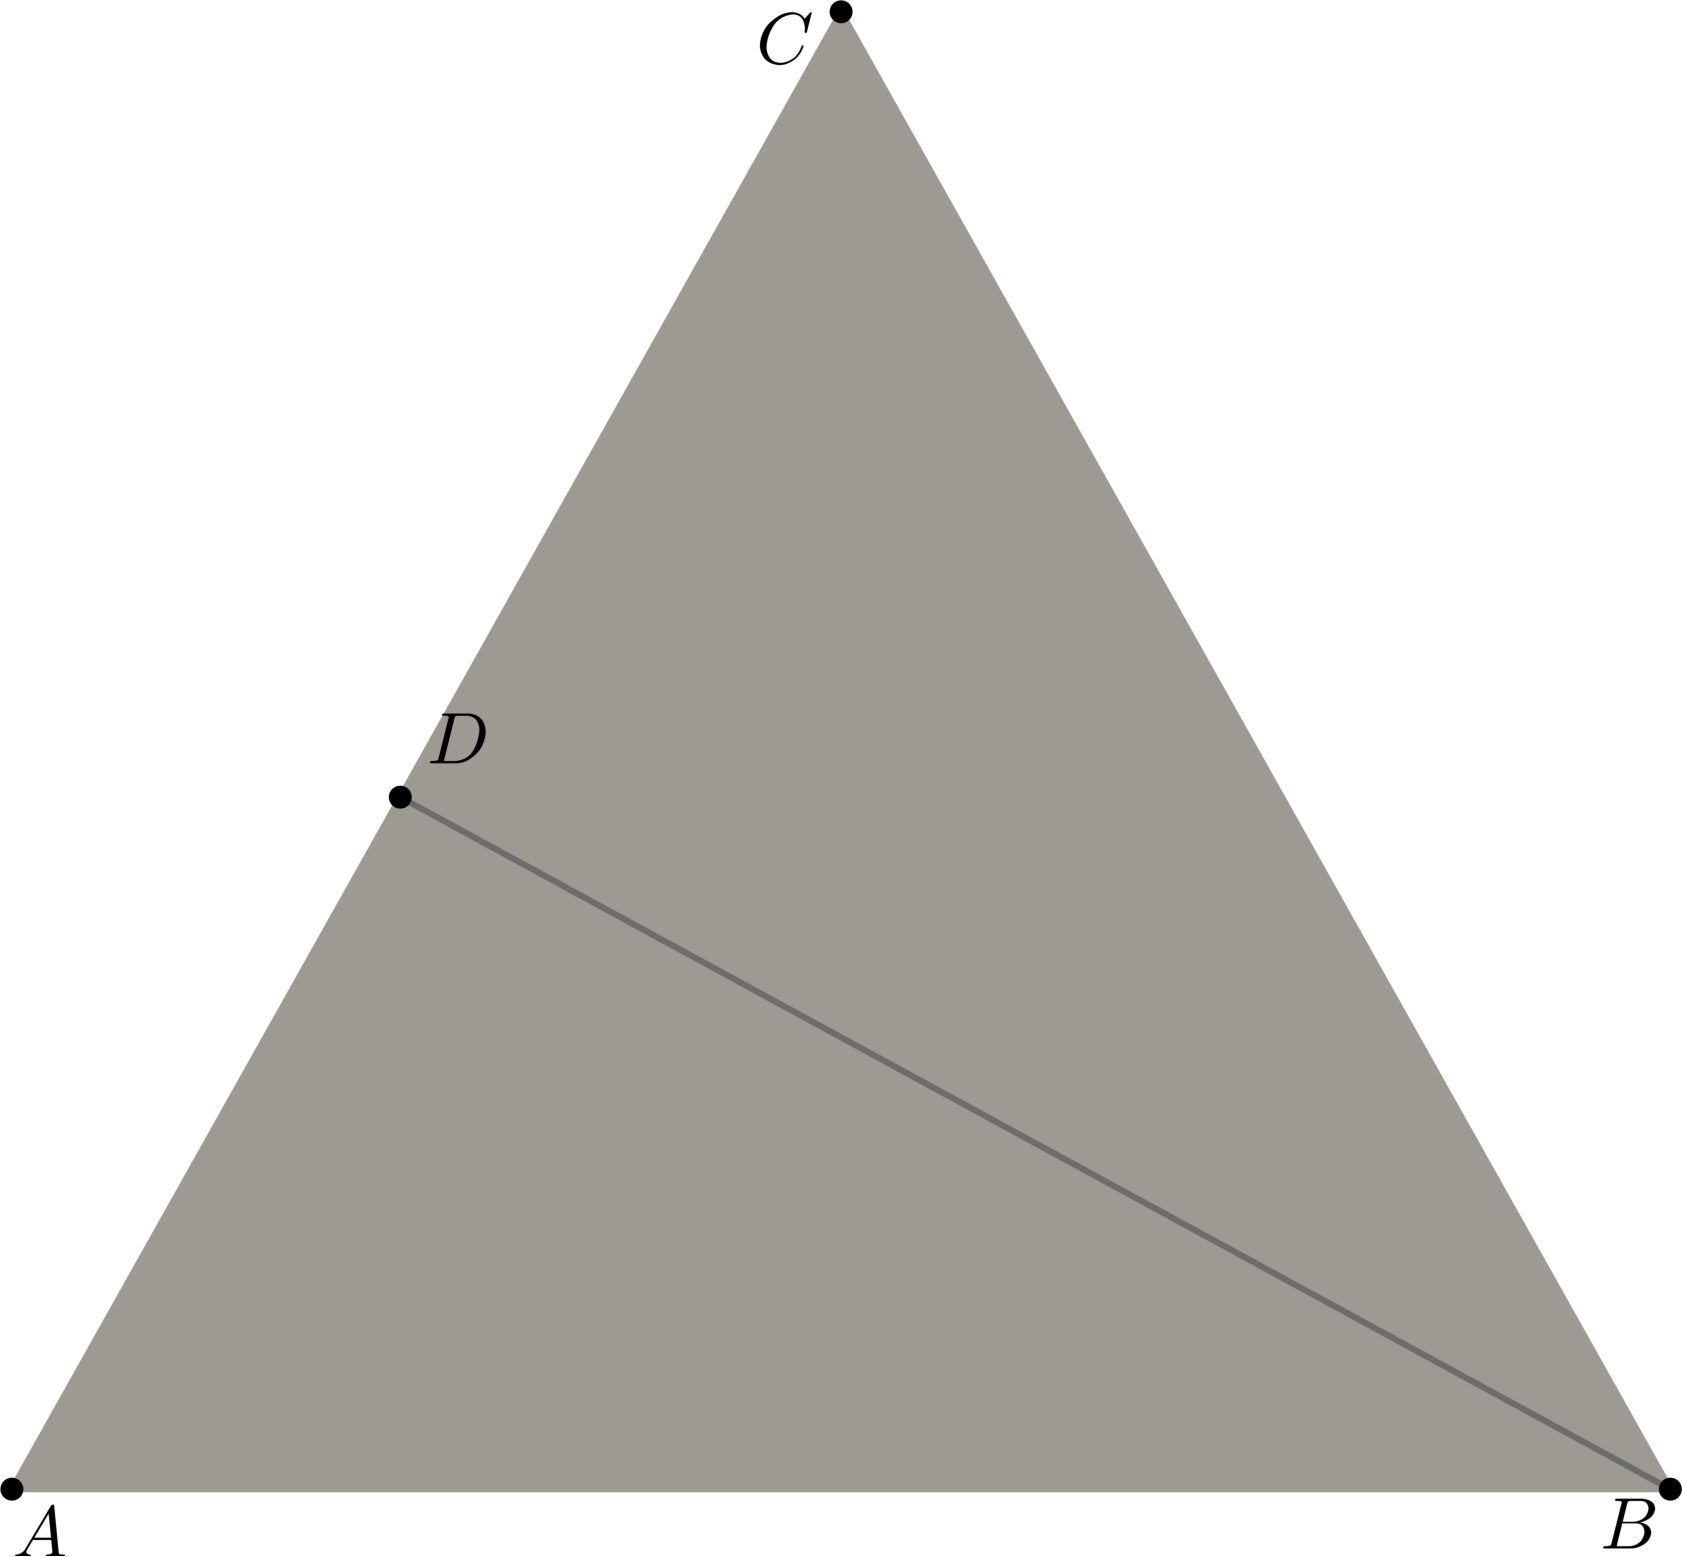
\includegraphics[width=\textwidth]{images/decoup_triangle-1.pdf}
    \caption{Insertion de $D$.}
    \label{fig:exemple_insert_pt_1}
\end{subfigure}
\\[0.5cm]
\begin{subfigure}{0.45\textwidth}
    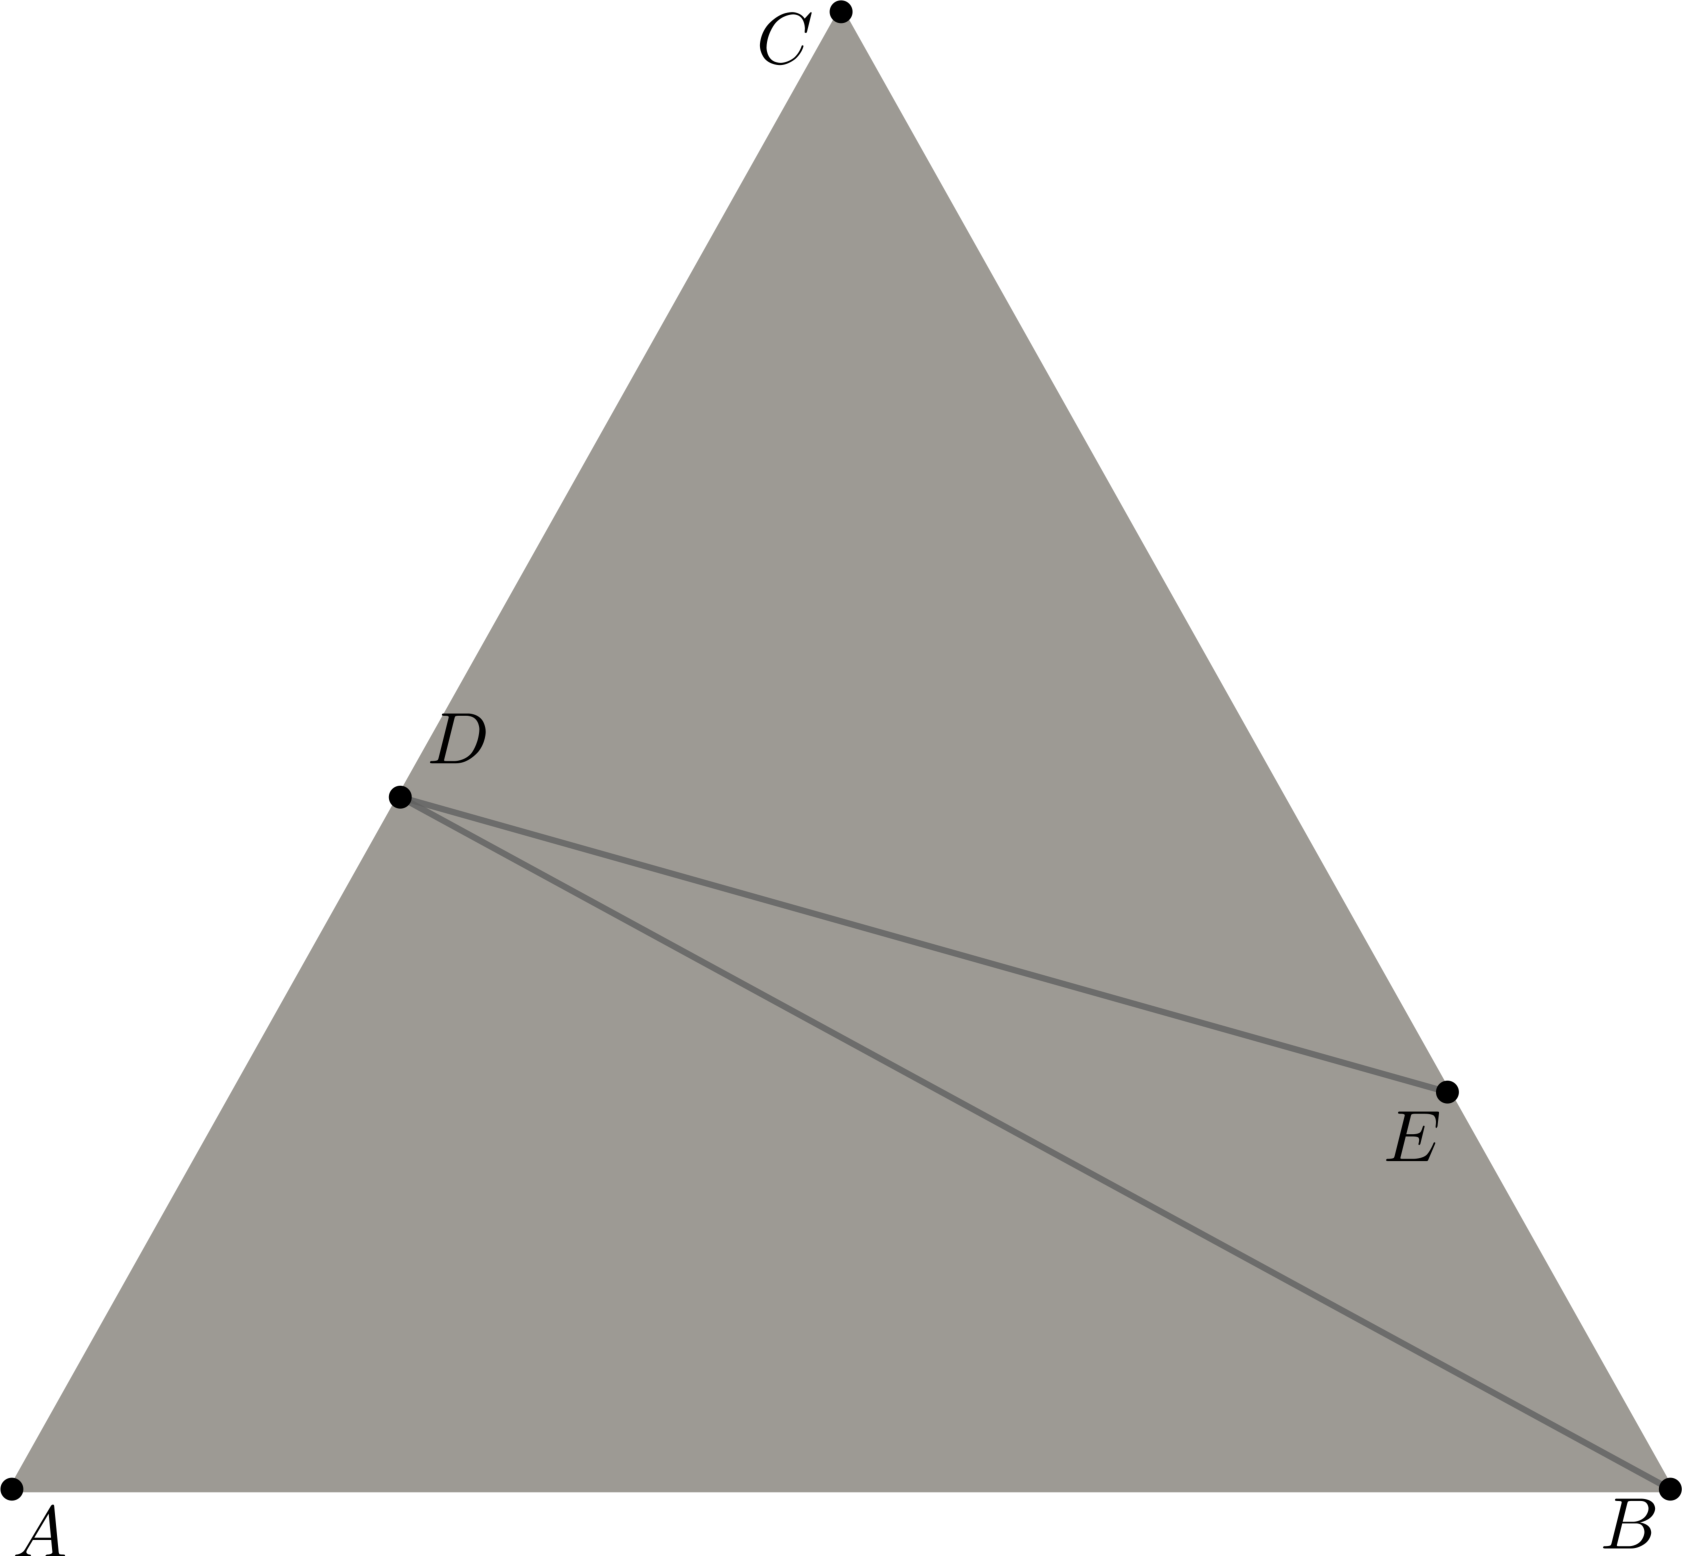
\includegraphics[width=\textwidth]{images/decoup_triangle-2.pdf}
    \caption{Insertion de $E$.}
    \label{fig:exemple_insert_pt_2}
\end{subfigure}
\hfill
\begin{subfigure}{0.45\textwidth}
    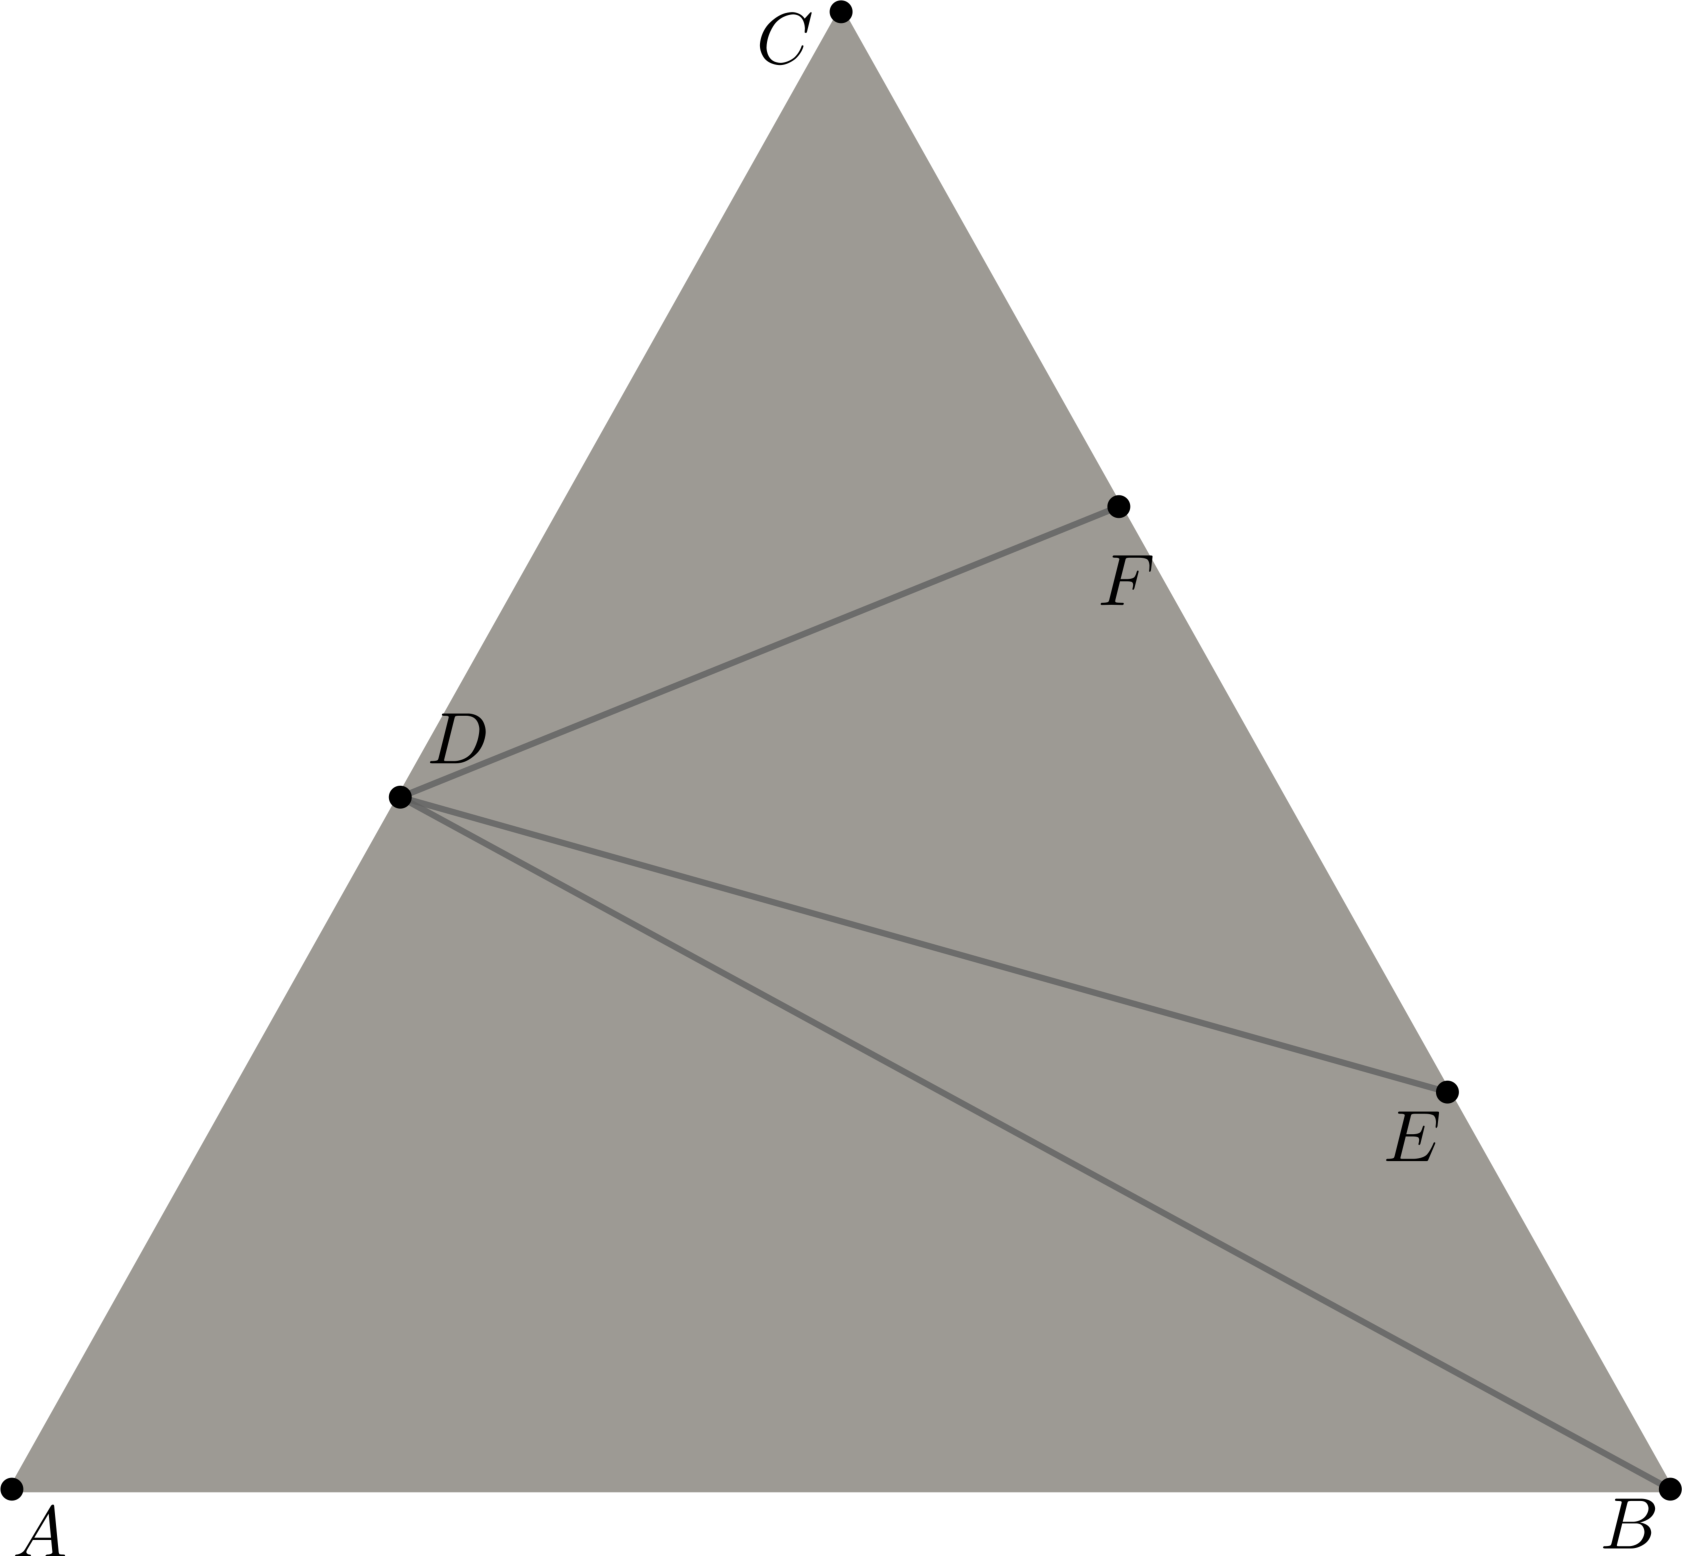
\includegraphics[width=\textwidth]{images/decoup_triangle-3.pdf}
    \caption{Insertion de $F$.}
    \label{fig:exemple_insert_pt_3}
\end{subfigure}
\\[0.5cm]
\begin{subfigure}{0.45\textwidth}
    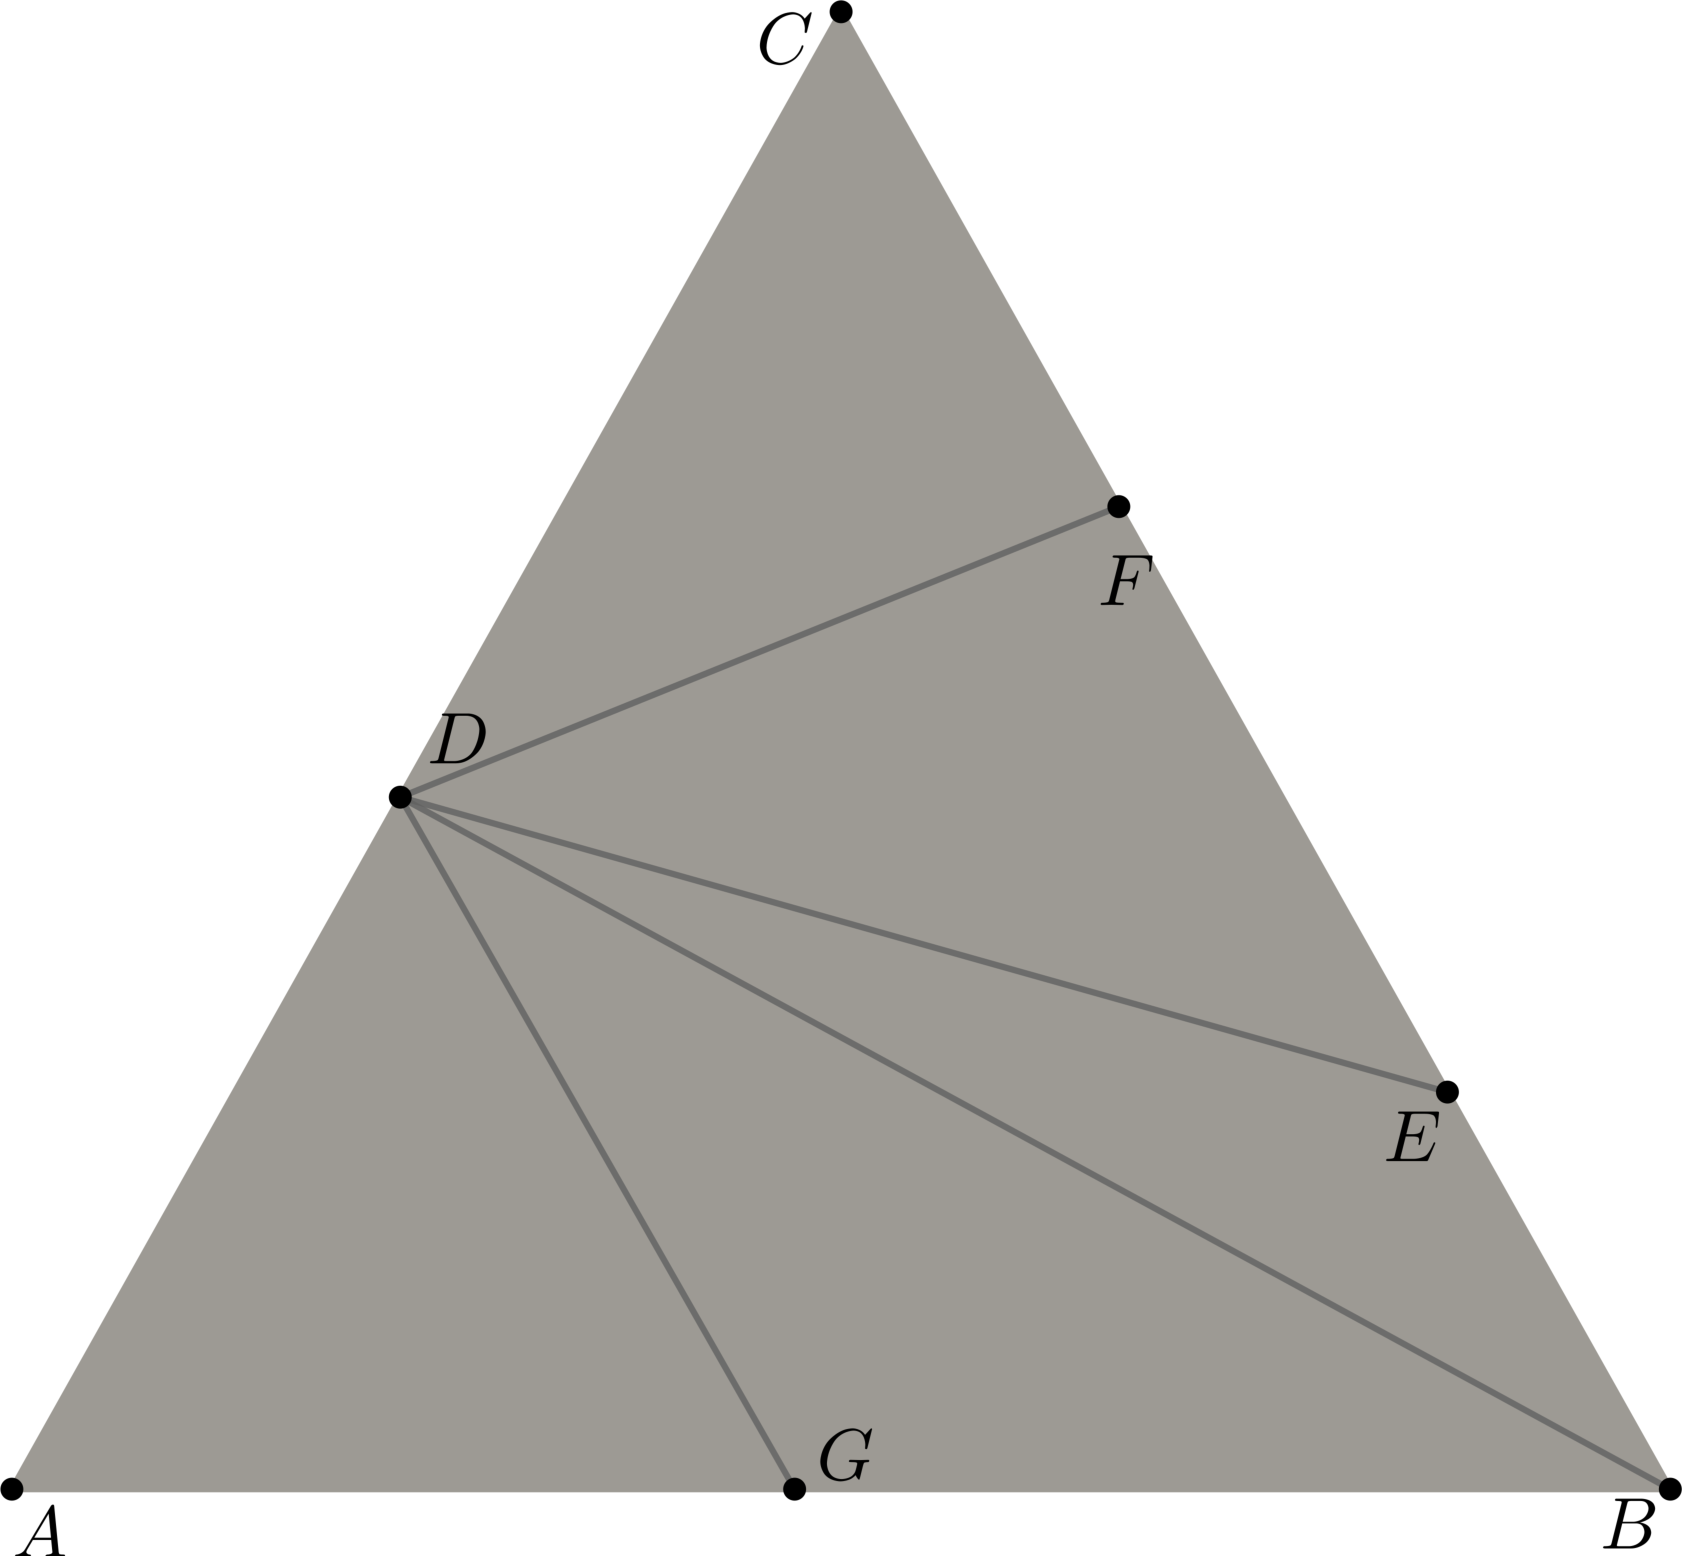
\includegraphics[width=\textwidth]{images/decoup_triangle-4.pdf}
    \caption{Insertion de $G$.}
    \label{fig:exemple_insert_pt_4}
\end{subfigure}
\hfill
\begin{subfigure}{0.45\textwidth}
    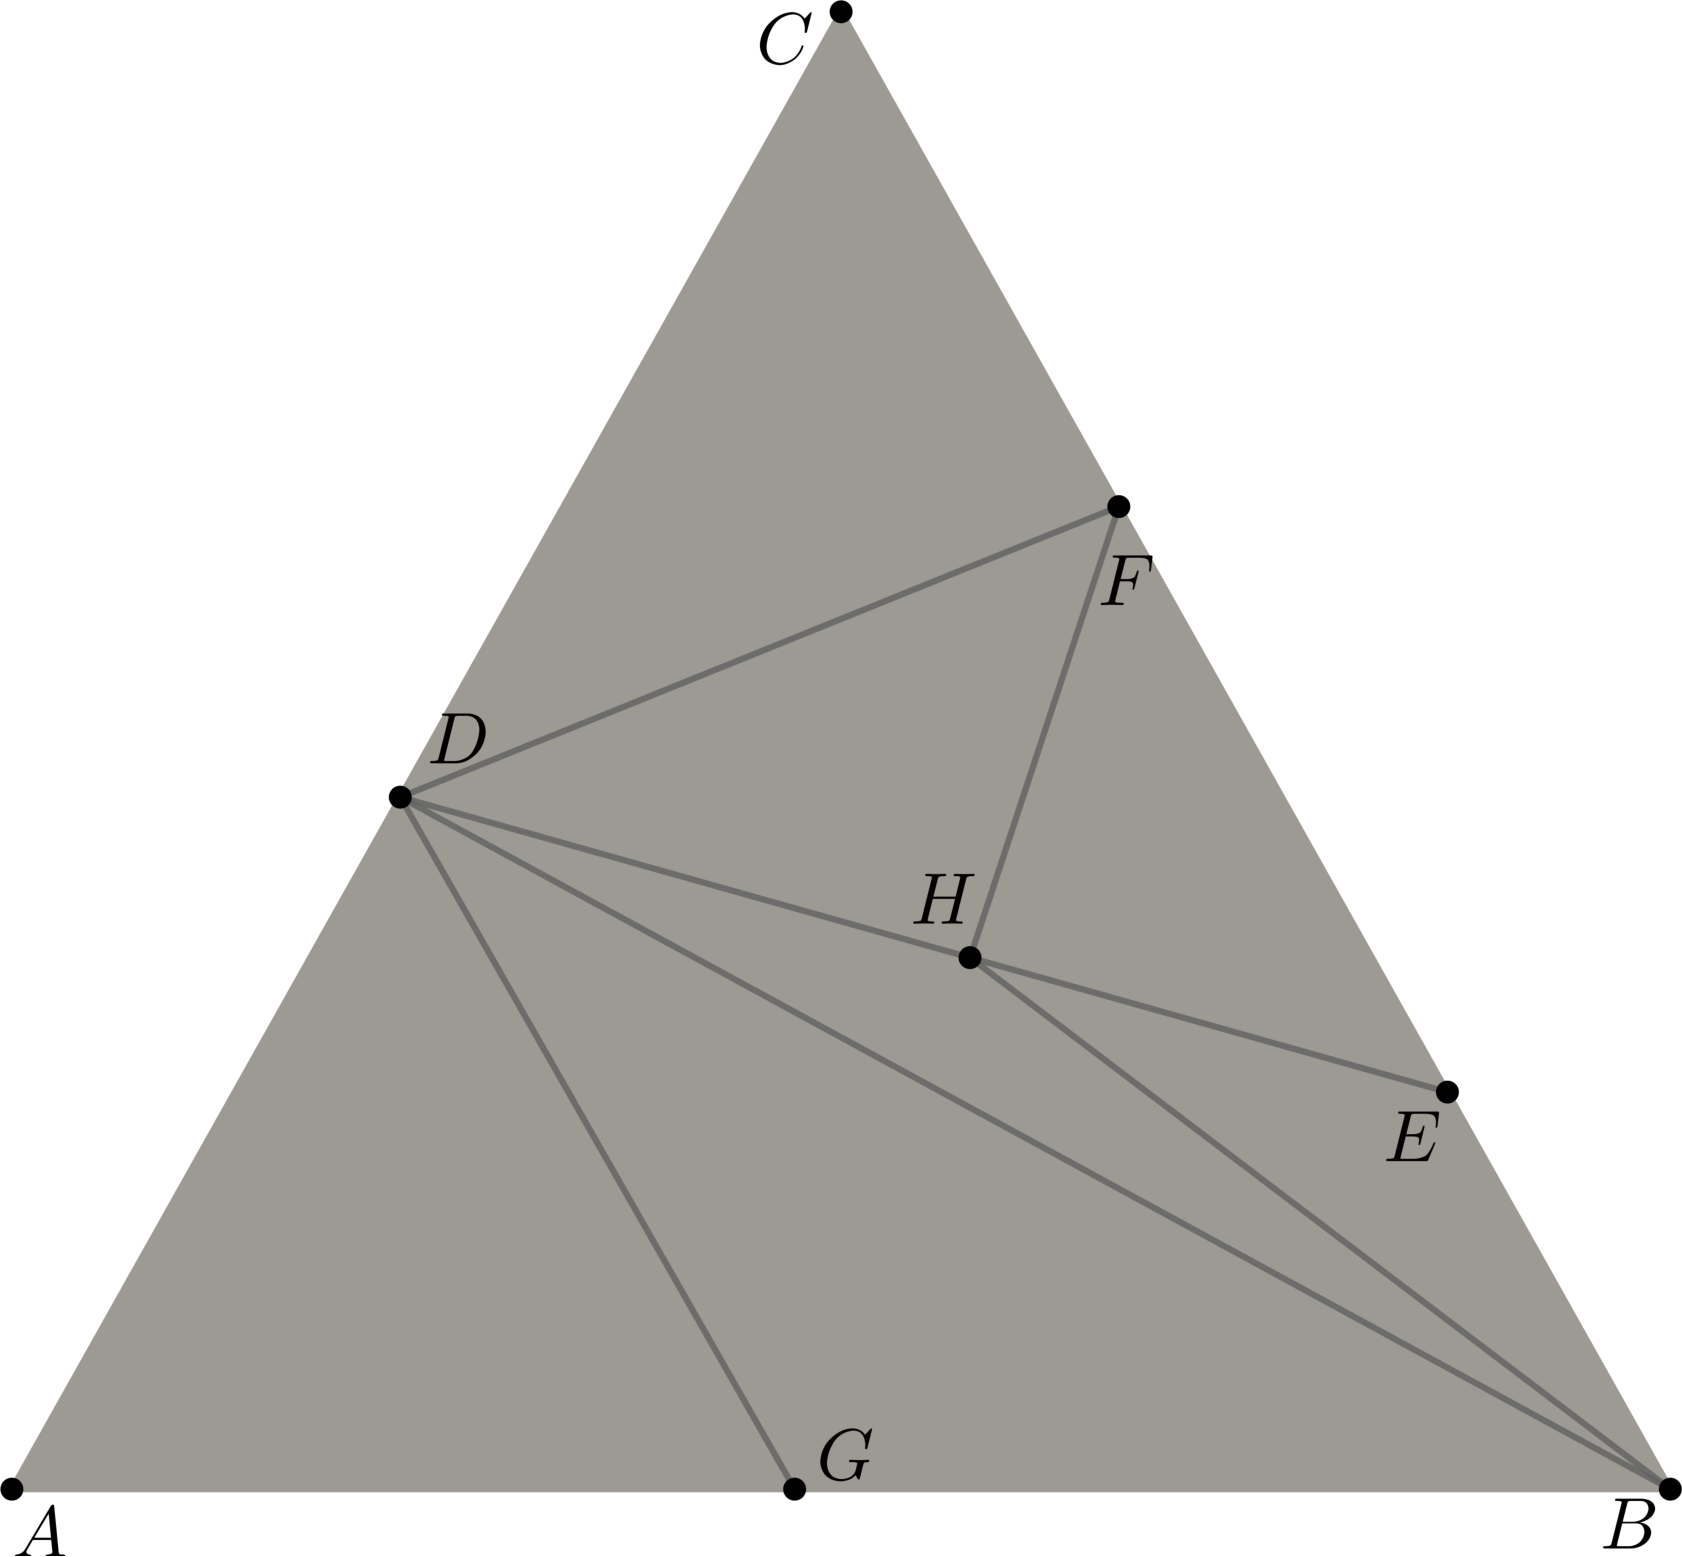
\includegraphics[width=\textwidth]{images/decoup_triangle-5.pdf}
    \caption{Insertion de $H$.}
    \label{fig:exemple_insert_pt_5}
\end{subfigure}
\caption{Adaptation locale du triangle en fonction des points de passage des séparatrices.}
\label{fig:exemple_insert_pt}
\end{figure}

Sur la figure illustrée par la référence \ref{fig:exemple_insert_pt}, nous avons quatre segments de séparatrices à considérer ($DH$, $HE$, $HG$, $FH$). Nous procédons donc à l'insertion séquentielle des points $D$, $E$, $F$, $G$, $H$ (l'ordre d'insertion est sans importance). On se retrouve alors avec un raffinement local contenant tous les points nécessaire à la suite du processus. Le raffinement ainsi produit ne contient pas en général dans la liste de ses arêtes les segments des séparatrices. La suite du processus consistera à recenser les segments des séparatrices qui n'ont pas été généré suite à l'insertion des points puis à procéder à des ajustements locaux pour garantir leur présence dans le raffinement effectué. Plus précisement, nous effectuerons des retournements d'arêtes en nous inspirant de la méthode de génération de maillages de type Voronoi, telle qu'exposée dans \cite{georgegeneration}: soit $T$ le maillage local correspondant au raffinement précédemment construit. Avec cette notation, nous identifions le triangle $T$ et son maillage local. Soit $AB$ un segment non présente dans $T$ et $T_{AB}$ l'ensemble des éléments de $T$ dont une arête est coupée par $AB$.

\begin{figure}[h!]
\centering
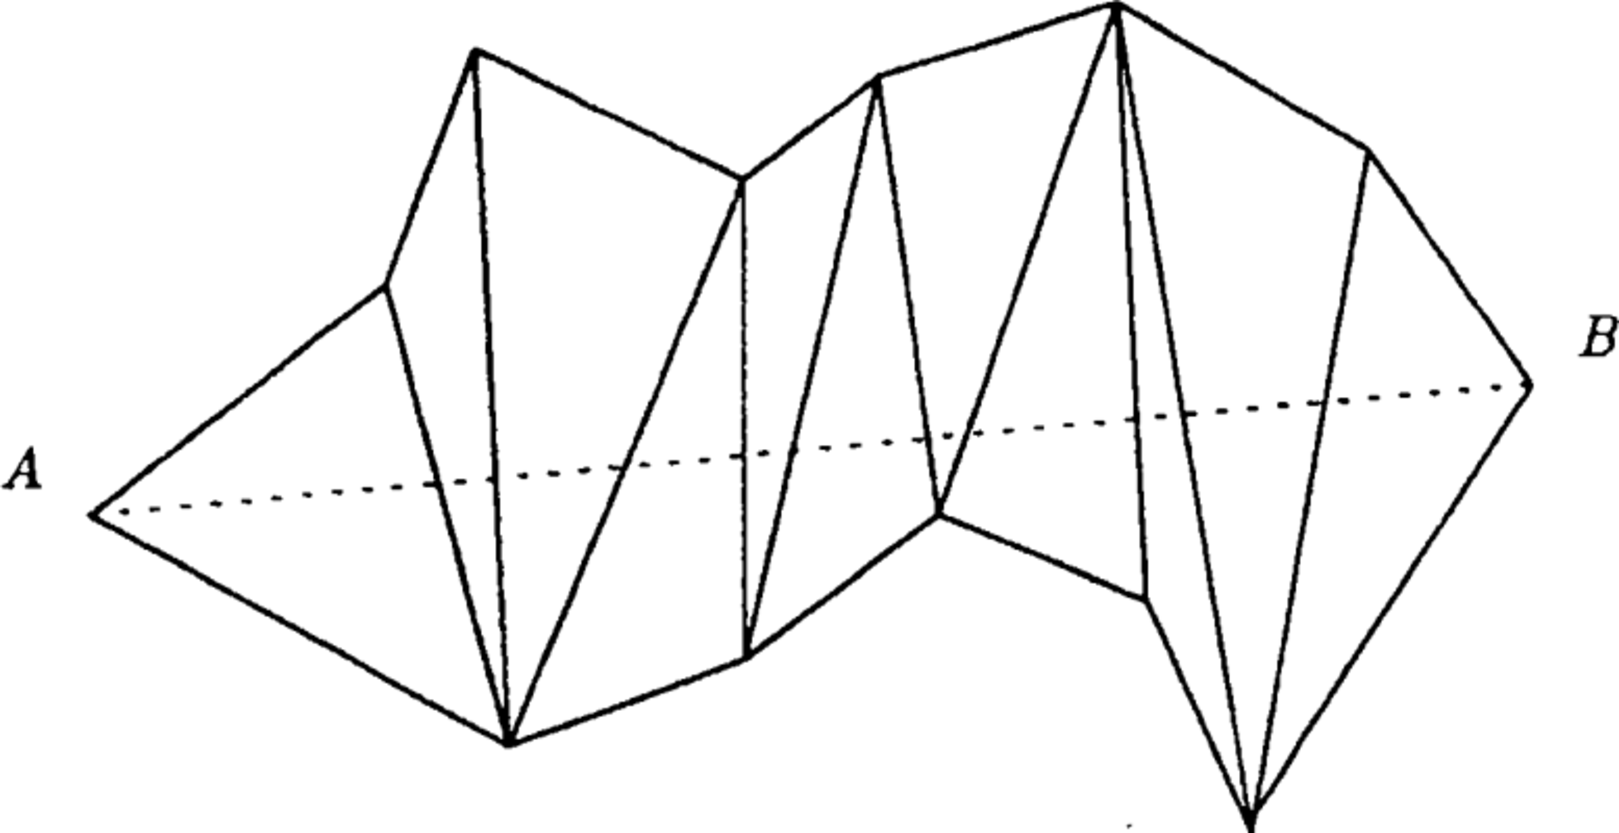
\includegraphics[scale=0.275]{images/retourn_arete_george-1.pdf}\hfill
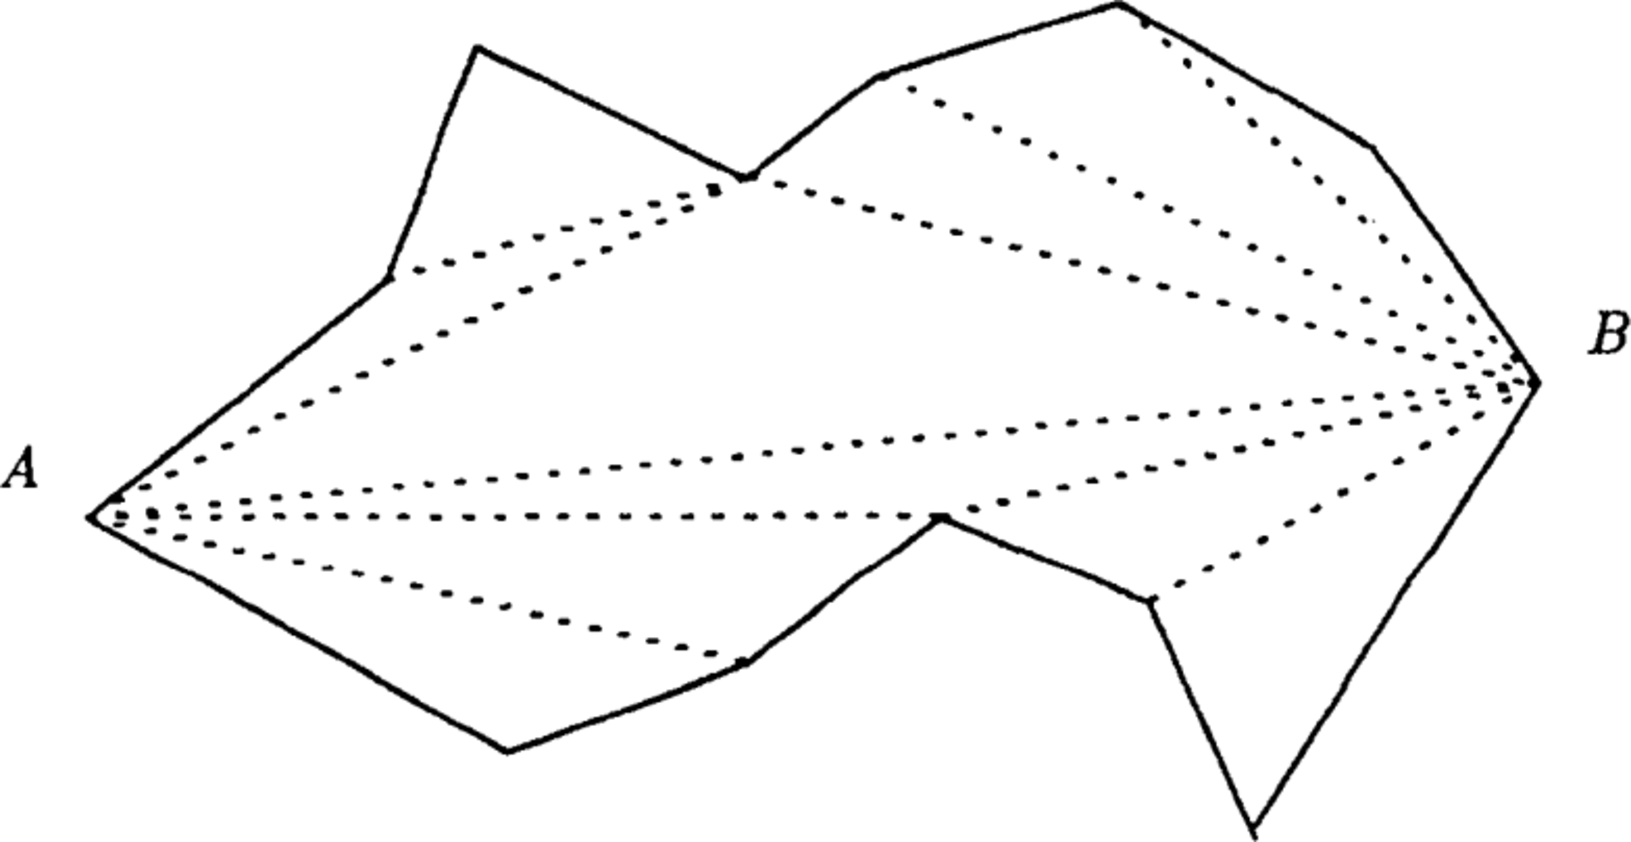
\includegraphics[scale=0.275]{images/retourn_arete_george-2.pdf}
\caption{Direction de sortie différentes.}
\label{fig:retournement_arete}
\end{figure}




\begin{figure}[h!]
\centering
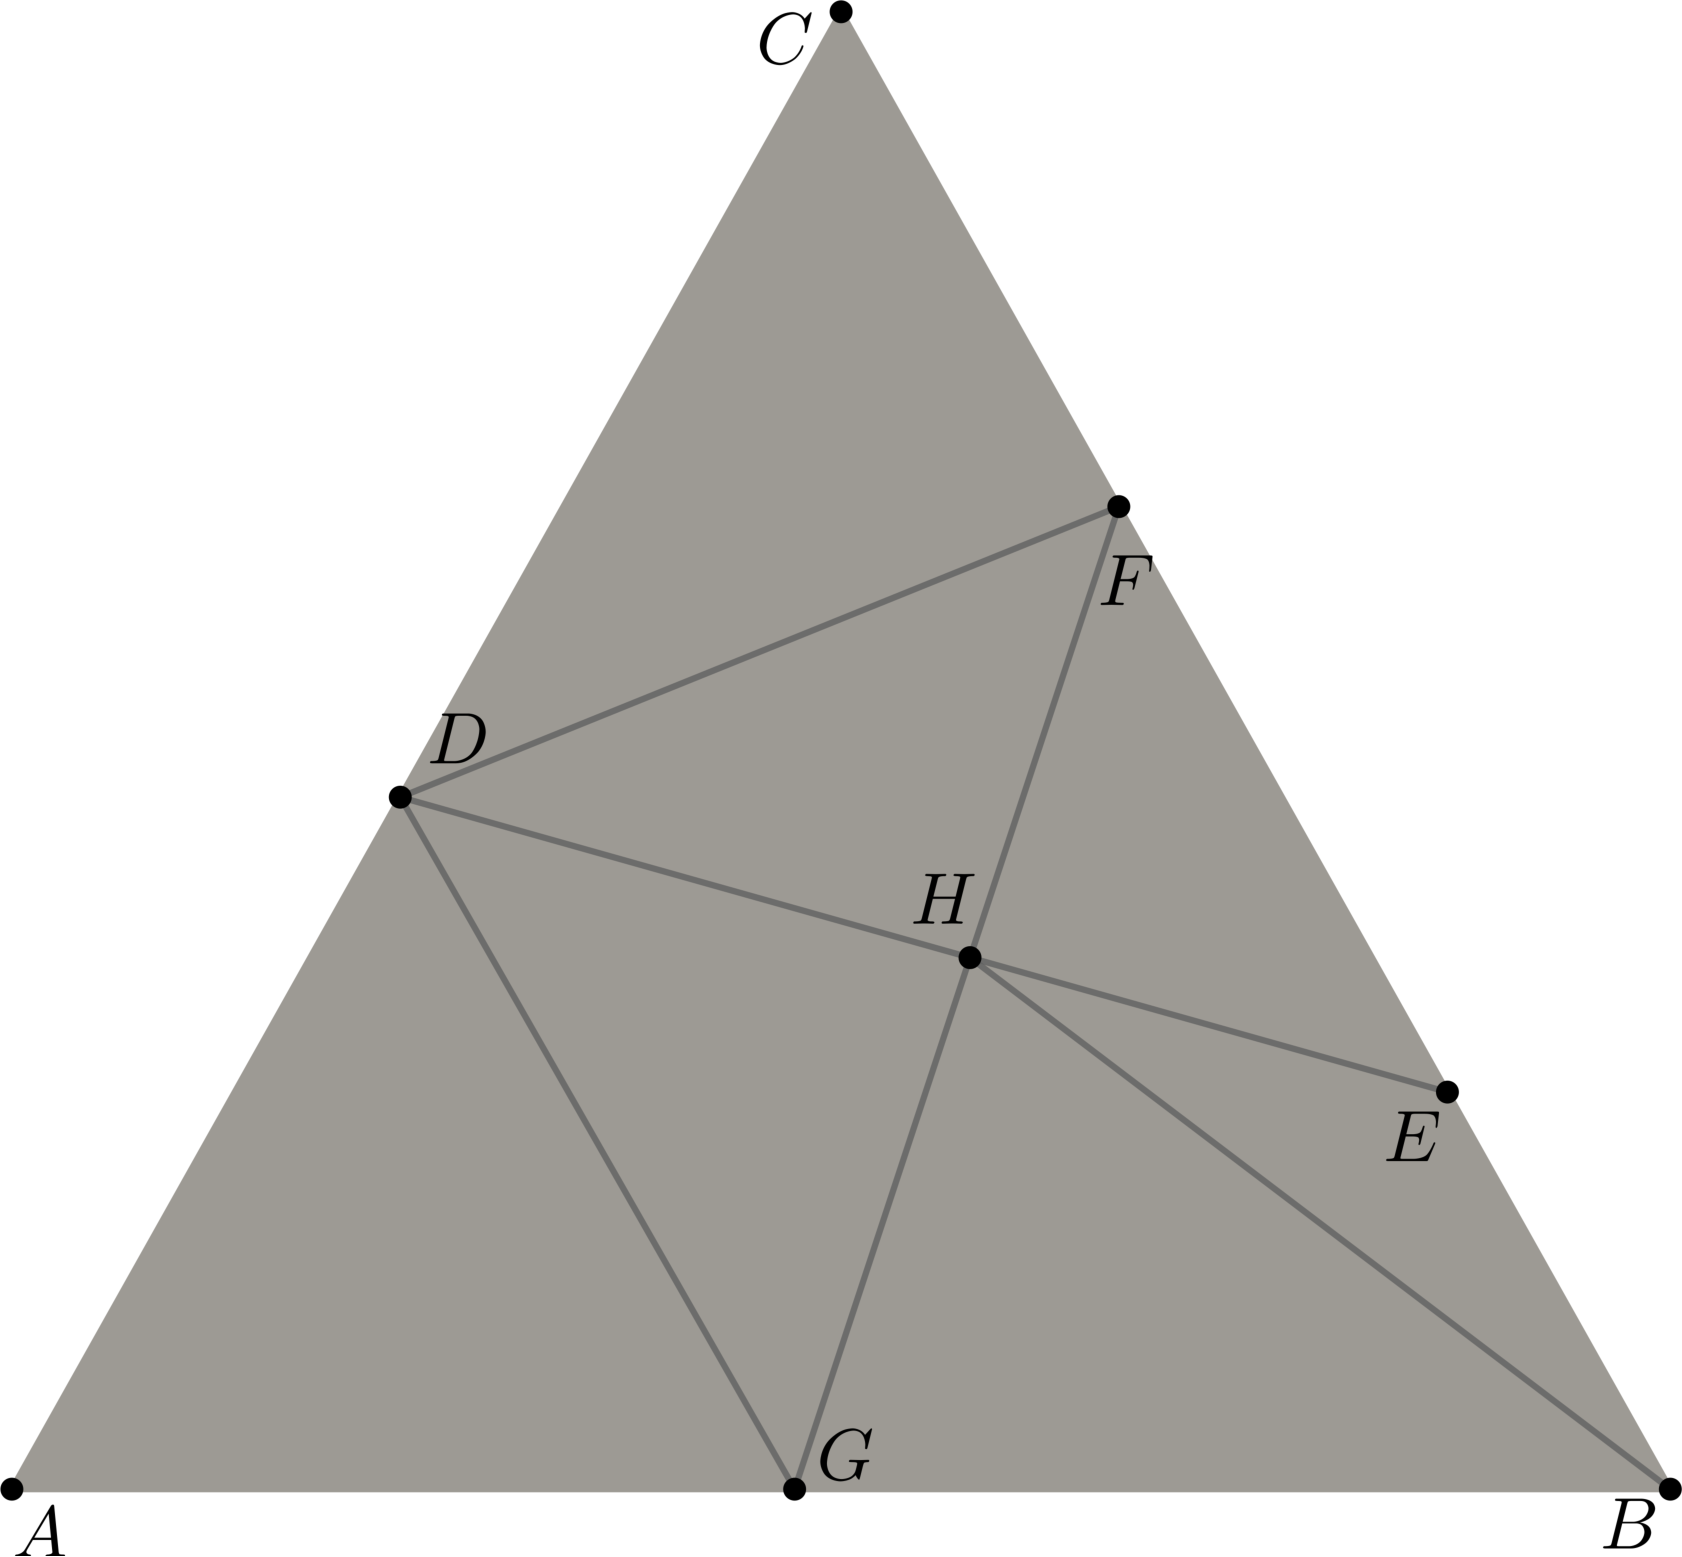
\includegraphics[scale=0.275]{images/retournement_arete-1.pdf}\hfill
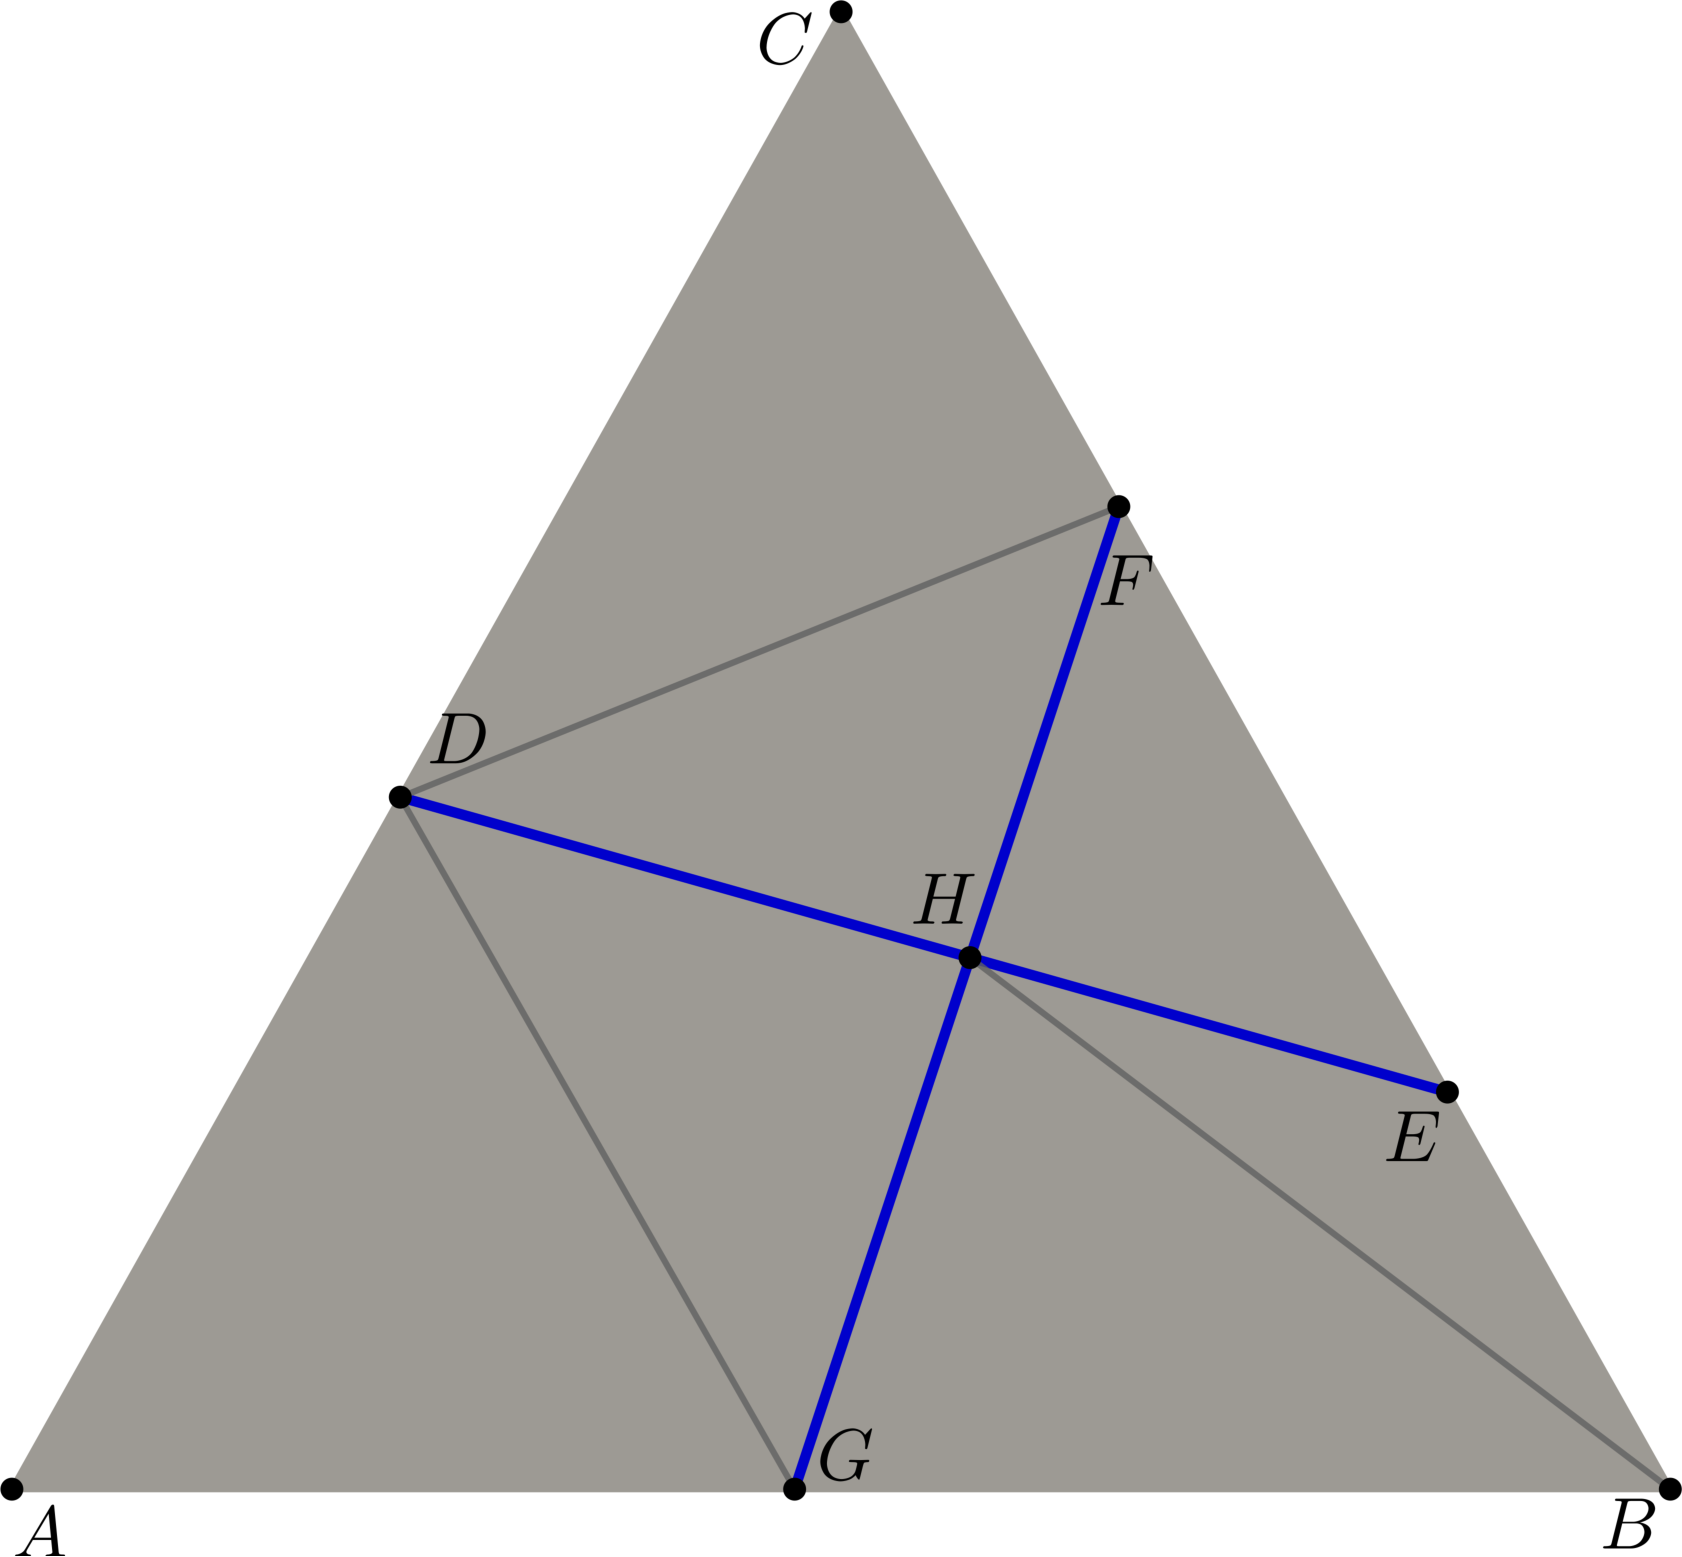
\includegraphics[scale=0.275]{images/retournement_arete-2.pdf}
\caption{Direction de sortie différentes. Source: \cite{georgegeneration}.}
\label{fig:retournement_arete}
\end{figure}


Localement dans chaque triangle,\\
on ajoute les points constituant les separatrices a $\Omega_h$ modifiant ainsi la topologie du maillage triangulaire initial,\\
Pour se faire, on exécute localement l'algorithme d'insertition de point localement dans chaque triangle.\\
donné par\\
En utilisant des opérations de retournement d'arêtes, nous cherchons ensuite à retrouver les segments constituant les séparatrices ayant traversé $T$. Cette procédure s'inspire de la génération de maillages selon la méthode de type Voronoi présentée dans \cite{georgegeneration}. Notons $K$\\
Il ne reste plus qu'a travailler chaque partition en la maillant \ref{subsec:gen_mesh_quad}
\begin{figure}[!h]
\centering
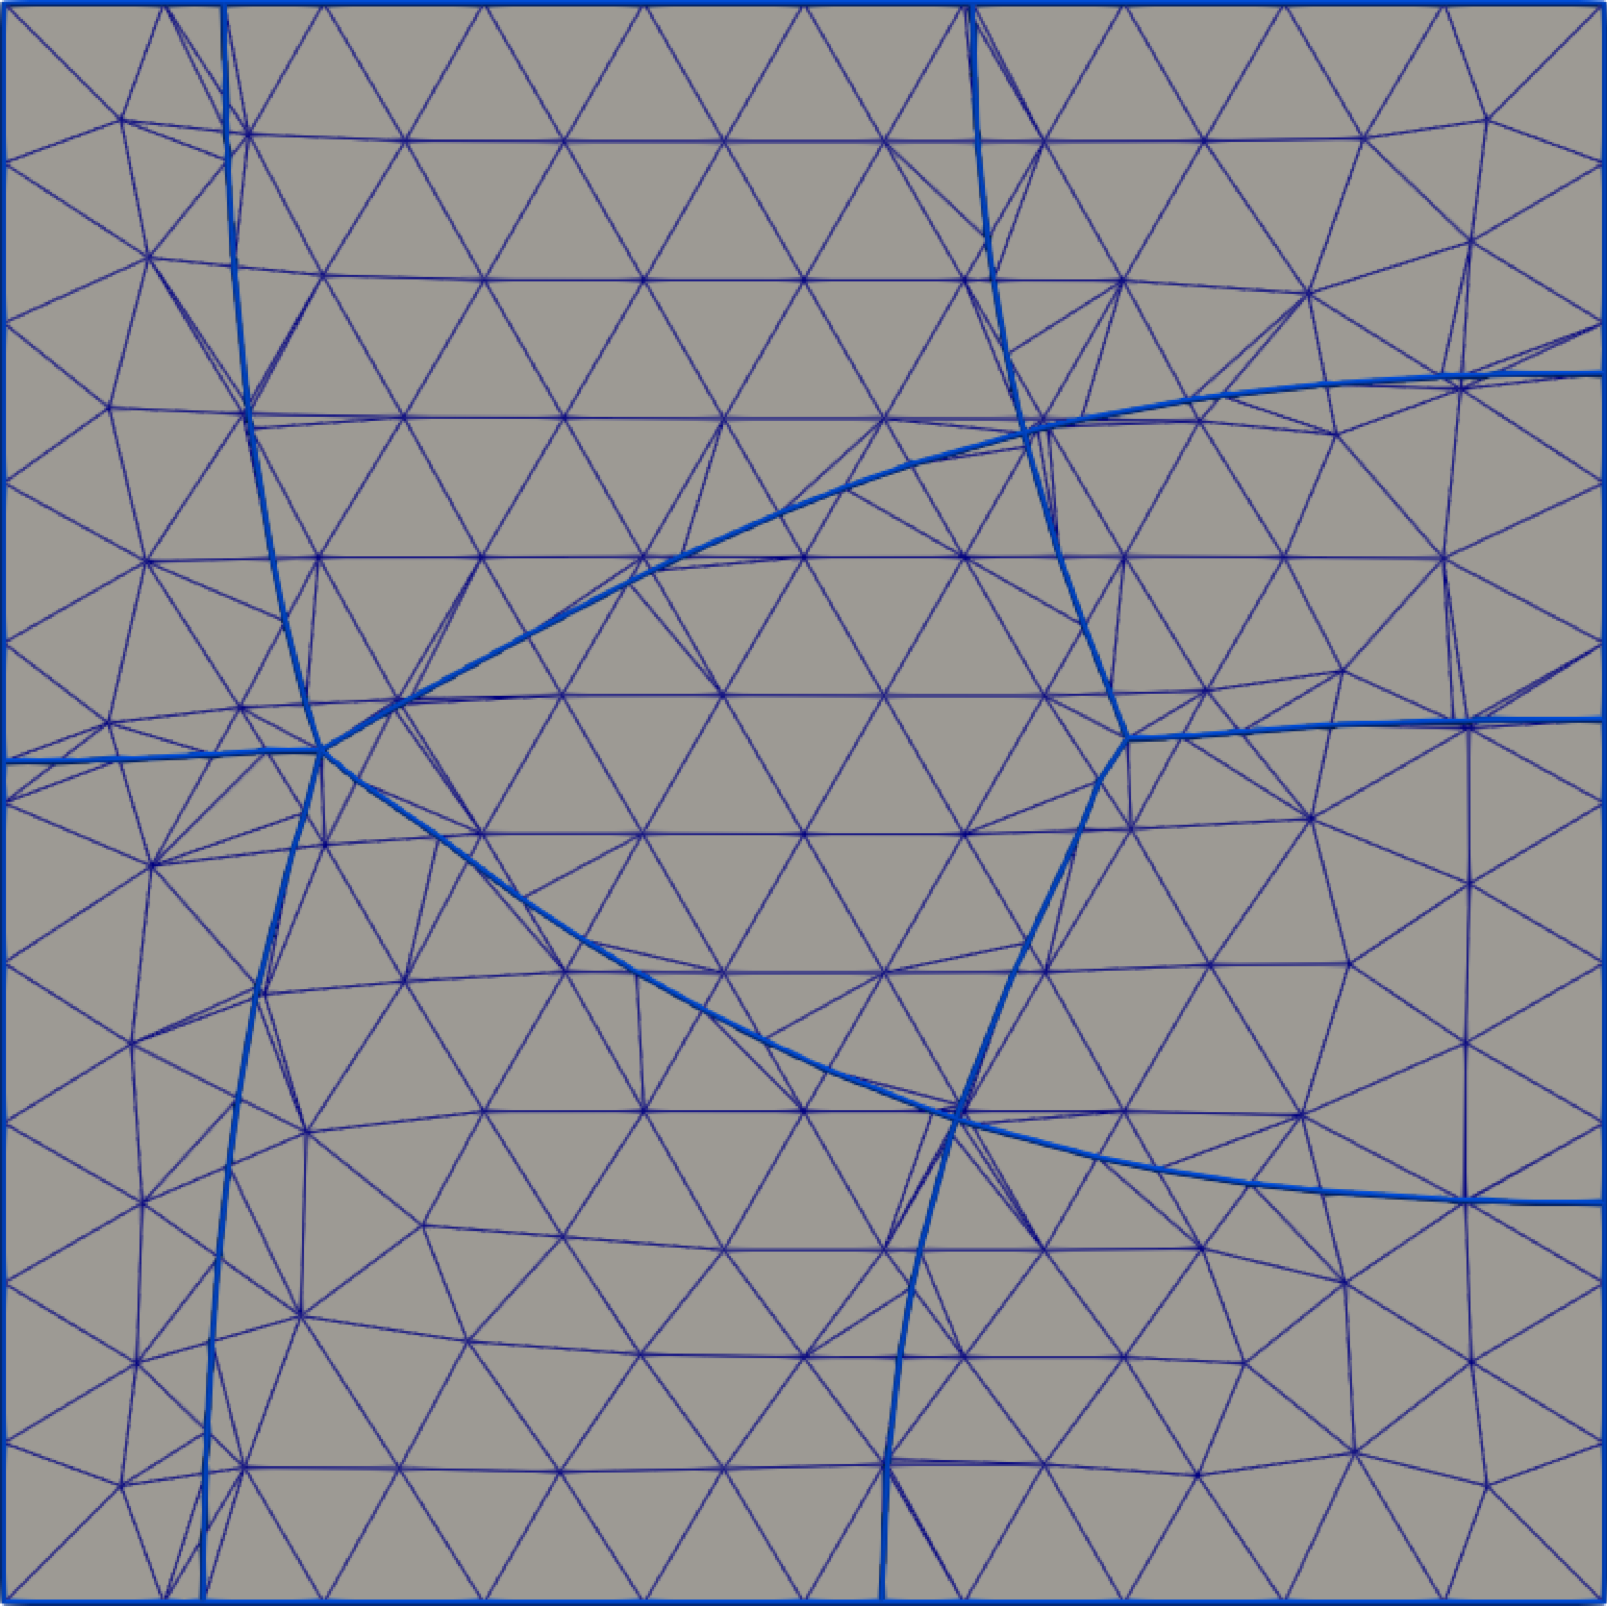
\includegraphics[scale=0.29]{images/eclatement_2.pdf}
\hfill
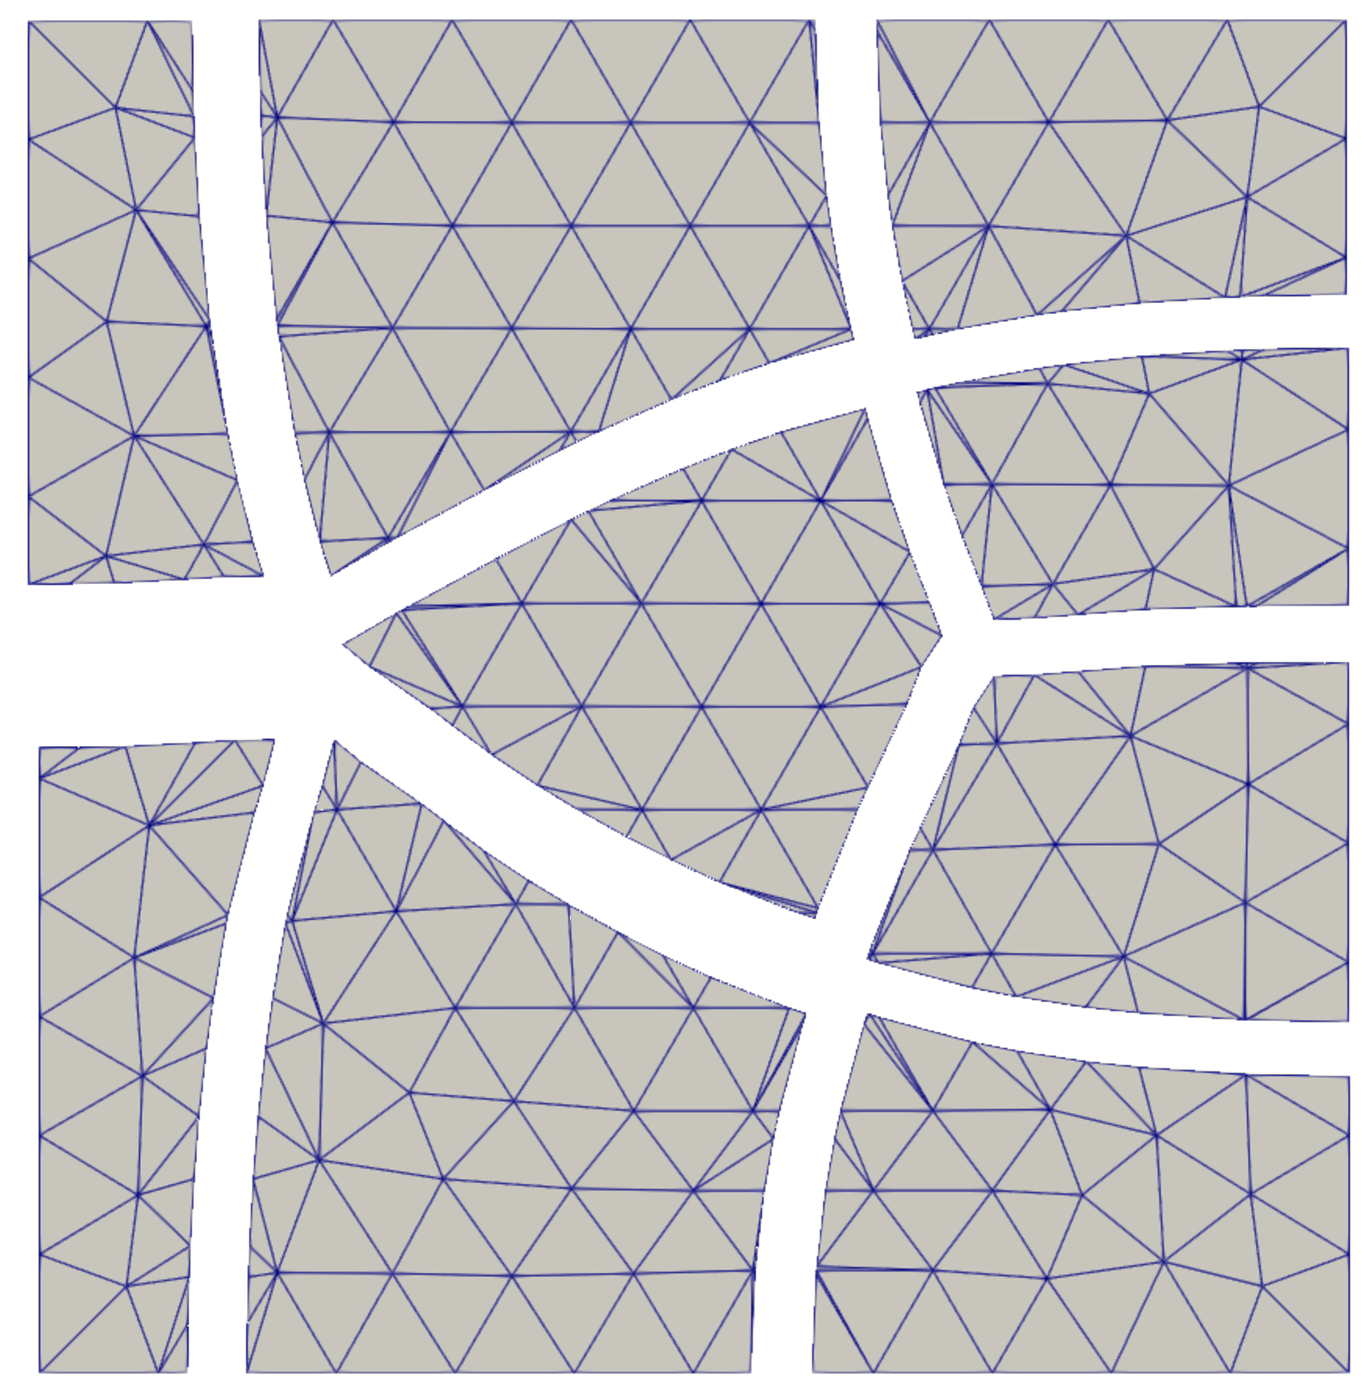
\includegraphics[scale=0.352]{images/eclatement_3.pdf}
\caption{Extraction des régions en tant que sous-maillages.}
\label{fig:eclatement}
\end{figure}

\subsection{Génération du maillage quadrilatéral}
\label{subsec:gen_mesh_quad}

equation\\
Tracé directement dans le champ de croix\\
Interpolation transfini.

\section{Opération d'alignement}
s'inspirer de kennan cos laplacien rtheta...
\[\]
Nous abordons maintenant la discrétisation de l'opération d'alignement présenté dans le chapitre \ref{chap:theoritical}. Étant donné une représentation $\bar{N}_h$ du champ de croix $\bar{N}$ sur le bord $\partial\Omega_h$ de $\Omega_h$, nous cherchons à modifier $\bar{u}_h$ en construisant un nouveau champ de croix $\bar{v}_h$ qui soit aligné avec $\partial\Omega_h$. Autrement dit, on veut que pour tout $p\in\partial\Omega_h$, $\bar{v}_h(p)\in\{\bar{N}_h(p), 0\}$. Pour se faire, on commence par définir l'ensemble des points singuliers de bord du champ de croix $\bar{v}$ que l'on note $\mathcal{B}$. On associe un paramètre $I_p$ pour tout $p\in\mathcal{B}$ représentant l'indice que nous souhaitons qu'il possède dans le champ de croix $\bar{v}$ et vérifiant:
\begin{equation}
I_p=
\left\{
\begin{array}{ll}
\displaystyle\frac{k}{4}\mbox{ avec }k\in\mathbb{Z}\mbox{ et }k\leq 1&\mbox{ si }p\in\mathcal{B},\\[0.5cm]
0&\mbox{ sinon }.
\end{array}
\right.
\end{equation}
Le champ de croix $\bar{u}_h$ choisit comme champ initial doit alors vérifié $0<\#\mathcal{S}_{\bar{u}_h}<\infty$ et pour tout point $p\in\mathcal{S}_{\bar{u}_h}$, $id_{\bar{u}_h}(p)=k/4$, avec $k\in\mathbb{Z}$ et $k\leq 1$. On suppose de plus que:
\begin{equation}
    \label{eqn:etude_hyp_u_simple}
    \theta_{\bar{u}_h}-\theta_{\bar{u}_h}=\chi(\Omega)-\sum_{p\in\mathcal{B}}I(p).
\end{equation}
Le champ de croix $\bar{v}_h$ est alors donné par:
\begin{equation}
\bar{v}_h(p)=
\left\{
\begin{array}{ll}
\mathbf{R}(\phi_h(p))\bar{u}_h(p) & \mbox{ si } p\in\Omega_h\backslash(\mathcal{B}\cup\mathcal{S}_{\bar{u}_h}),\\[0.5cm]
\bar{N}_h(p) & \mbox{ si } p\in(\mathcal{S}_{\bar{u}_h}\cap\partial\Omega_h)\backslash\mathcal{B},\\[0.5cm]
0 & \mbox{ si } p\in\mathcal{B}.
\end{array}
\right.
\label{eqn:etude_def_v_second}
\end{equation}
où $\phi_h$ est une approximation de la fonction $\phi$ définie par l'équation de Laplace suivant:\begin{equation}
\left\{
\begin{array}{lcll}
\Delta\phi &=& 0 &\mbox{ dans }\Omega_h,\\[0.5cm]
\phi_h(\gamma(t))&=&\theta^\gamma_{\bar{N}_h}(t)+\mathcal{I}(t)-\theta_{\bar{u}_h}(\gamma(t)) & \mbox{ sur } \gamma^{-1}(\partial\Omega_h\backslash(\mathcal{B}\cup\mathcal{S}_{\bar{u}_h})),
\end{array}
\right.
\end{equation}
où $\gamma$ est une paramétrisation sur $[0, 1]$ de $\partial\Omega_h$ et la fonction $\mathcal{I}$ est donnée par:
$$
\mathcal{I}(t)=\displaystyle\sum_{s\in\gamma^{-1}(\mathcal{B})}\left[\left(\pi-\widehat{\gamma(s)}-2\pi I_{\gamma(s)}\right)-\left(\displaystyle\lim\limits_{r\rightarrow s^+}\theta^{\gamma}_{\bar{N}_h}(r) - \lim\limits_{r\rightarrow s^-}\theta^{\gamma}_{\bar{N}_h}(r)\right)\right]\mathbb{1}_{[0, t]}(s),
$$
avec $\widehat{\gamma(s)}$ la mesure de l'ouverture angulaire de la frontière en $\gamma(s)$.

ne pas oublié thetah pour le non-simplement connexe

